% Initial and revised submissions should be 12 point; this will be removed in the final version.
%\documentclass[12pt]{TD-CJS}
\documentclass{article}

% Initial and revised submissions should also be double spaced.  This command will be removed in the final version.
%\renewcommand{\baselinestretch}{2}

\usepackage{latexsym}
\usepackage{amsmath}
\usepackage{amsfonts}
\usepackage{amssymb}
\usepackage{psfrag}
\usepackage{graphicx}
\usepackage[dvipsnames]{xcolor}
\usepackage{url}
\usepackage{float}
\usepackage[margin=1in]{geometry}
% header.tex
% this is where you load pacakges, specify custom formats, etc.

% \usepackage{changepage}
\usepackage{amsmath,amsthm,amssymb,amsfonts}
\usepackage{mathtools}
\usepackage{bbm}
% enumitem for custom lists
\usepackage{enumitem}
% Load dsfont this to get proper indicator function (bold 1) with \mathds{1}:
\usepackage{dsfont}
\usepackage{centernot}
\usepackage{appendix}

% set up graphics
\usepackage{graphicx}
\DeclareGraphicsExtensions{.pdf,.png,.jpg}
\graphicspath{ {fig/} }
% defs.tex
% this is where you define custom notation, commands, etc.

\DeclareMathOperator*{\argmax}{arg\,max}
\DeclareMathOperator*{\argmin}{arg\,min}
\DeclareMathOperator*{\del}{\nabla}

%%
% full alphabets of different styles
%%

% bf series
\def\bfA{\mathbf{A}}
\def\bfB{\mathbf{B}}
\def\bfC{\mathbf{C}}
\def\bfD{\mathbf{D}}
\def\bfE{\mathbf{E}}
\def\bfF{\mathbf{F}}
\def\bfG{\mathbf{G}}
\def\bfH{\mathbf{H}}
\def\bfI{\mathbf{I}}
\def\bfJ{\mathbf{J}}
\def\bfK{\mathbf{K}}
\def\bfL{\mathbf{L}}
\def\bfM{\mathbf{M}}
\def\bfN{\mathbf{N}}
\def\bfO{\mathbf{O}}
\def\bfP{\mathbf{P}}
\def\bfQ{\mathbf{Q}}
\def\bfR{\mathbf{R}}
\def\bfS{\mathbf{S}}
\def\bfT{\mathbf{T}}
\def\bfU{\mathbf{U}}
\def\bfV{\mathbf{V}}
\def\bfW{\mathbf{W}}
\def\bfX{\mathbf{X}}
\def\bfY{\mathbf{Y}}
\def\bfZ{\mathbf{Z}}

% bb series
\def\bbA{\mathbb{A}}
\def\bbB{\mathbb{B}}
\def\bbC{\mathbb{C}}
\def\bbD{\mathbb{D}}
\def\bbE{\mathbb{E}}
\def\bbF{\mathbb{F}}
\def\bbG{\mathbb{G}}
\def\bbH{\mathbb{H}}
\def\bbI{\mathbb{I}}
\def\bbJ{\mathbb{J}}
\def\bbK{\mathbb{K}}
\def\bbL{\mathbb{L}}
\def\bbM{\mathbb{M}}
\def\bbN{\mathbb{N}}
\def\bbO{\mathbb{O}}
\def\bbP{\mathbb{P}}
\def\bbQ{\mathbb{Q}}
\def\bbR{\mathbb{R}}
\def\bbS{\mathbb{S}}
\def\bbT{\mathbb{T}}
\def\bbU{\mathbb{U}}
\def\bbV{\mathbb{V}}
\def\bbW{\mathbb{W}}
\def\bbX{\mathbb{X}}
\def\bbY{\mathbb{Y}}
\def\bbZ{\mathbb{Z}}

% cal series
\def\calA{\mathcal{A}}
\def\calB{\mathcal{B}}
\def\calC{\mathcal{C}}
\def\calD{\mathcal{D}}
\def\calE{\mathcal{E}}
\def\calF{\mathcal{F}}
\def\calG{\mathcal{G}}
\def\calH{\mathcal{H}}
\def\calI{\mathcal{I}}
\def\calJ{\mathcal{J}}
\def\calK{\mathcal{K}}
\def\calL{\mathcal{L}}
\def\calM{\mathcal{M}}
\def\calN{\mathcal{N}}
\def\calO{\mathcal{O}}
\def\calP{\mathcal{P}}
\def\calQ{\mathcal{Q}}
\def\calR{\mathcal{R}}
\def\calS{\mathcal{S}}
\def\calT{\mathcal{T}}
\def\calU{\mathcal{U}}
\def\calV{\mathcal{V}}
\def\calW{\mathcal{W}}
\def\calX{\mathcal{X}}
\def\calY{\mathcal{Y}}
\def\calZ{\mathcal{Z}}

\def\bfTheta{\mathbf{\Theta}}


%%%%%%%%%%%%%%%%%%%%%%%%%%%%%%%%%%%%%%%%%%%%%%%%%%%%%%%%%%
% text short-cuts
\def\iid{i.i.d.\ } %i.i.d.
\def\ie{i.e.\ }
\def\eg{e.g.\ }
\def\Polya{P\'{o}lya\ }
%%%%%%%%%%%%%%%%%%%%%%%%%%%%%%%%%%%%%%%%%%%%%%%%%%%%%%%%%%

%%%%%%%%%%%%%%%%%%%%%%%%%%%%%%%%%%%%%%%%%%%%%%%%%%%%%%%%%%
% quasi-universal probabilistic and mathematical notation
% my preferences (modulo publication conventions, and clashes like random vectors):
%   vectors: bold, lowercase
%   matrices: bold, uppercase
%   operators: blackboard (e.g., \mathbb{E}), uppercase
%   sets, spaces: calligraphic, uppercase
%   random variables: normal font, uppercase
%   deterministic quantities: normal font, lowercase
%%%%%%%%%%%%%%%%%%%%%%%%%%%%%%%%%%%%%%%%%%%%%%%%%%%%%%%%%%

% operators
\def\P{\bbP} %fundamental probability
\def\E{\bbE} %expectation
% conditional expectation
\DeclarePairedDelimiterX\bigCond[2]{[}{]}{#1 \;\delimsize\vert\; #2}
\newcommand{\conditional}[3][]{\bbE_{#1}\bigCond*{#2}{#3}}
\def\Law{\mathcal{L}} %law; this is by convention in the literature
\def\indicator{\mathds{1}} % indicator function

% sets and groups
\def\borel{\calB} %Borel sets
\def\sigAlg{\calA} %sigma-algebra
\def\filtration{\calF} %filtration
\def\grp{\calG} %group

% binary relations
\def\condind{{\perp\!\!\!\perp}} %independence/conditional independence
\def\equdist{\stackrel{\text{\rm\tiny d}}{=}} %equal in distribution
\def\equas{\stackrel{\text{\rm\tiny a.s.}}{=}} %euqal amost surely
\def\simiid{\sim_{\mbox{\tiny iid}}} %sampled i.i.d

% common vectors and matrices
\def\onevec{\mathbf{1}}
\def\iden{\mathbf{I}} % identity matrix
\def\supp{\text{\rm supp}}

% misc
% floor and ceiling
\DeclarePairedDelimiter{\ceilpair}{\lceil}{\rceil}
\DeclarePairedDelimiter{\floor}{\lfloor}{\rfloor}
\newcommand{\argdot}{{\,\vcenter{\hbox{\tiny$\bullet$}}\,}} %generic argument dot
%%%%%%%%%%%%%%%%%%%%%%%%%%%%%%%%%%%%%%%%%%%%%%%%%%%%%%%%%%

%%%%%%%%%%%%%%%%%%%%%%%%%%%%%%%%%%%%%%%%%%%%%%%%%%%%%%%%%%
%% some distributions
% continuous
\def\UnifDist{\text{\rm Unif}}
\def\BetaDist{\text{\rm Beta}}
\def\ExpDist{\text{\rm Exp}}
\def\GammaDist{\text{\rm Gamma}}
% \def\GenGammaDist{\text{\rm GGa}} %Generalized Gamma

% discrete
\def\BernDist{\text{\rm Bernoulli}}
\def\BinomDist{\text{\rm Binomial}}
\def\PoissonPlus{\text{\rm Poisson}_{+}}
\def\PoissonDist{\text{\rm Poisson}}
\def\NBPlus{\text{\rm NB}_{+}}
\def\NBDist{\text{\rm NB}}
\def\GeomDist{\text{\rm Geom}}
% \def\CRP{\text{\rm CRP}}
% \def\EGP{\text{\rm EGP}}
% \def\MittagLeffler{\text{\rm ML}}
%%%%%%%%%%%%%%%%%%%%%%%%%%%%%%%%%%%%%%%%%%%%%%%%%%%%%%%%%%

%%%%%%%%%%%%%%%%%%%%%%%%%%%%%%%%%%%%%%%%%%%%%%%%%%%%%%%%%%
% Project-specific notation should go here
% (Because it's at the end of the file, it can overwrite anything that came before.)

%e.g.,
\def\Laplacian{\calL}
\def\P{\calP}

% combinatorial objects
\def\perm{\sigma} %fixed permutation
\def\Perm{\Sigma} %random permutation
\def\part{\pi} %fixed partition
\def\Part{\Pi} %random partition


%%%%%%%%%%%%%%%%%%%%%%%%%%%%%%%%%%%%%%%%%%%%%%%%%%%%%%%%%%

\begin{document}
%\firstpage{1}
%\lastpage{25}
%\jvol{xx}
%\issue{yy}
%\jyear{2020}
%\jid{CJS}
%\aid{???}
% The running head contains the author names
%\rhauthor{BlindedA and BlindedB}
%\copyrightline{Statistical Society of Canada}
%\Frenchcopyrightline{Soci\'et\'e statistique du Canada}
% History: received and accepted dates
%\received{\rec{9}{July}{2009}}
%\accepted{\acc{8}{July}{2010}}

% User-defined commands go here
%\renewcommand{\eqref}[1]{(\ref{#1})}
%\newcommand{\mb}[1]{\mathbf{#1}}
%\newcommand{\mbb}[1]{\mathbb{#1}}
%\newcommand{\mt}[1]{\mathrm{#1}}
%\newcommand{\rv}{random variable}
%\newcommand{\newblock}{}
\bibliographystyle{abbrvnat}

% Title, authors, affiliations
\title{Modelling state-switching functional data with hidden Markov models: supplementary material (simulation study)}%\query{Q1}
\date{}
\author{BlindedA, BlindedB}%\authorref{1}\thanksref{*}}
%\author{BlindedB}%\authorref{2}}
%\affiliation[1]{Author affiliations will go here in the accepted manuscript, but do NOT include them in your initial submission because it must be anonymous.}
%\affiliation[2]{Second Affiliation}

% Abstract, keywords, and classification codes

\maketitle

\newcounter{tablenum}
\addtocounter{tablenum}{1}
\newcounter{fignum}
\addtocounter{fignum}{1}

%\section{Simulation Study Results}

    \section{Simulated Data}
    
        \begin{center}
    	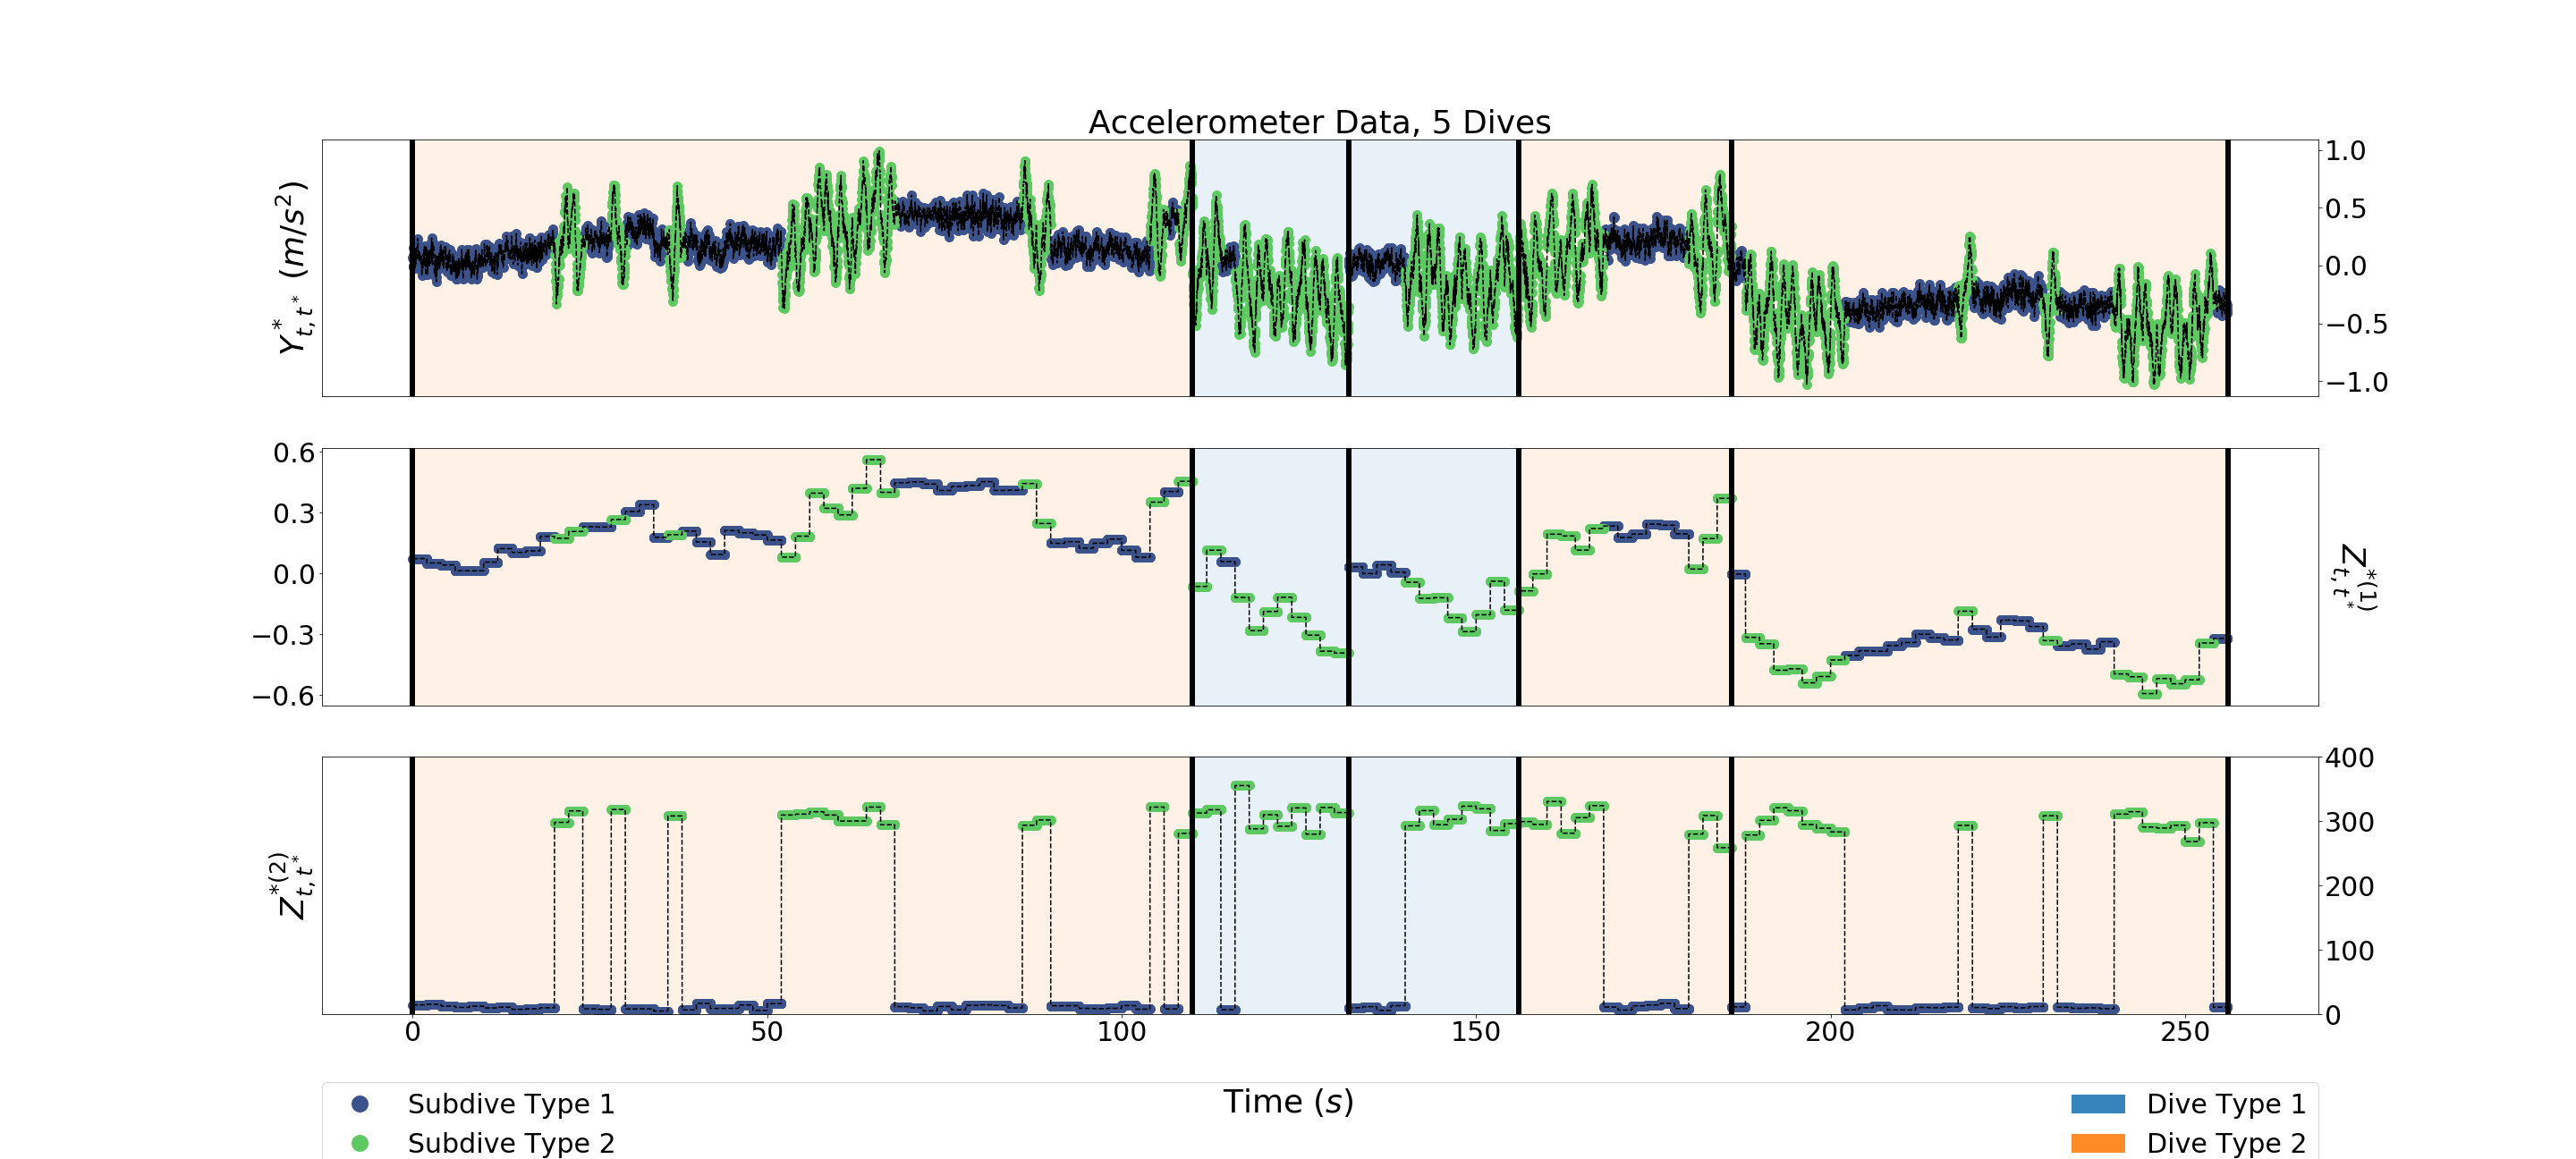
\includegraphics[width=5in]{../Plots/sim_data.png}
    	\end{center}
    	
    	\noindent Figure \arabic{fignum}: Acceleration data for a five dives of a selected simulated data set. The raw accelerometer data is denoted as $Y^*_{t,\tilde t^*}$ and recorded at 50 times per second while $\Zone_{t,\tilde t^*}$ and $\Ztwo_{t,\tilde t^*}$ are recorded at once every two seconds. Dives are separated by vertical black lines. The colour of the curve corresponds to the true fine-scale state, while the colour of the background corresponds to the true dive type. Subdive state 1 can plausibly be interpreted as ``gliding", subdive state 2 can plausibly be interpreted as active swimming, and subdive state 3 can be interpretted as sudden or aggressive movement.
    	\addtocounter{fignum}{1}

    \newpage
    \section{Accuracy comparisons}
        
        \begin{center}
        \scalebox{0.75}{
        \bgroup
        \def\arraystretch{1.5}
\begin{tabular}{ccccccc}
Model                       & \multicolumn{1}{c}{Train Time (m)} & \multicolumn{1}{c}{Dive Type} & \multicolumn{1}{c}{Subdive Type} & \multicolumn{1}{c}{Dive Accuracy} & \multicolumn{1}{c}{Subdive Accuracy}  \\ \hline
\multirow{7}{*}{CarHHMM-DFT}& \multirow{7}{*}{$156 \pm 67$}   & All                           & All                              & $0.956 \pm 0.028$                   & $0.911 \pm 0.006$                       \\
                            &                                    & 1                             & 1                                & \multirow{3}{*}{$0.973\pm0.032$}    & $0.846 \pm 0.027$                       \\
                            &                                    & 1                             & 2                                &                                   & $0.918 \pm 0.011$                       \\ 
                            &                                    & 1                             & 3                                &                                   & $0.860 \pm 0.030$                       \\ 
                            &                                    & 2                             & 1                                & \multirow{3}{*}{$0.856\pm0.097$}    & $0.949 \pm 0.010$                       \\ 
                            &                                    & 2                             & 2                                &                                   & $0.915 \pm 0.015$                       \\
                            &                                    & 2                             & 3                                &                                   & $0.871 \pm 0.057$                       \\ \hline
\multirow{7}{*}{HHMM-DFT}   & \multirow{7}{*}{$162 \pm 64$}   & All                           & All                              & $0.959 \pm 0.025$                   & $0.844 \pm 0.024$                       \\
                            &                                    & 1                             & 1                                & \multirow{3}{*}{$0.977\pm0.028$}    & $0.761 \pm 0.063$                       \\ 
                            &                                    & 1                             & 2                                &                                   & $0.845 \pm 0.029$                       \\ 
                            &                                    & 1                             & 3                                &                                   & $0.858 \pm 0.034$                       \\
                            &                                    & 2                             & 1                                & \multirow{3}{*}{$0.851\pm0.097$}    & $0.883 \pm 0.066$                       \\ 
                            &                                    & 2                             & 2                                &                                   & $0.829 \pm 0.041$                       \\
                            &                                    & 2                             & 3                                &                                   & $0.876 \pm 0.061$                       \\ \hline
\multirow{7}{*}{CarHHMM}    & \multirow{7}{*}{$258 \pm 106$}   & All                           & All                              & $0.924 \pm 0.127$                   & $0.845 \pm 0.018$                       \\
                            &                                    & 1                             & 1                                & \multirow{3}{*}{$0.933\pm0.153$}    & $0.689 \pm 0.050$                       \\ 
                            &                                    & 1                             & 2                                &                                   & $0.900 \pm 0.031$                       \\ 
                            &                                    & 1                             & 3                                &                                   & $0.673 \pm 0.059$                       \\
                            &                                    & 2                             & 1                                & \multirow{3}{*}{$0.864\pm0.134$}    & $0.906 \pm 0.022$                       \\ 
                            &                                    & 2                             & 2                                &                                   & $0.848 \pm 0.033$                       \\
                            &                                    & 2                             & 3                                &                                   & $0.687 \pm 0.105$                       \\ \hline
\multirow{7}{*}{CarHMM-DFT} & \multirow{7}{*}{$45 \pm 22$}   & All                           & All                              & ---                                   & $0.912 \pm 0.006$                       \\
                            &                                    & 1                             & 1                                & \multirow{3}{*}{---          }    & $0.854 \pm 0.026$                       \\
                            &                                    & 1                             & 2                                &                                   & $0.921 \pm 0.011$                       \\                            
                            &                                    & 1                             & 3                                &                                   & $0.860 \pm 0.032$                       \\ 
                            &                                    & 2                             & 1                                & \multirow{3}{*}{---          }    & $0.943 \pm 0.011$                       \\ 
                            &                                    & 2                             & 2                                &                                   & $0.919 \pm 0.014$                       \\ 
                            &                                    & 2                             & 3                                &                                   & $0.878 \pm 0.053$                       \\ \hline
\end{tabular}
        \egroup
        }
        \end{center}
        
        \noindent Table \arabic{tablenum}: Average decoding accuracies and training times for all models used to categorize dive type and subdive state in the simulation study. Each of the four models was fit to 500 training data sets comprised of 100 simulated dives and tested on test data sets also comprised of 100 simulated dives. Reported values are averages, and $\pm$ refers to the sample standard deviation across the 500 data sets. Rows labelled Both/Both correspond to overall average decoding accuracy.
        \addtocounter{tablenum}{1}

    \newpage
    \section{Empirical joint distributions - dive duration ($Y_t$)}

        \begin{center}
        \scalebox{0.75}{
        \bgroup
        \centering
        \def\arraystretch{1.5}
\begin{tabular}{ccccccc}
Model                       & \multicolumn{1}{c}{Parameter} & \multicolumn{1}{c}{Dive Type} & \multicolumn{1}{c}{Estimate}   & \multicolumn{1}{c}{Bias}   & \multicolumn{1}{c}{Empirical SE}   & \multicolumn{1}{c}{Observed Fischer SE}     \\ \hline
\multirow{4}{*}{CarHHMM-DFT}& \multirow{2}{*}{$\mu_Y$}      & 1                             & $27.337$                         & $0.067$ $(p=0.287)$          & $1.393$                             & $1.025 \pm 0.124$                             \\
                            &                               & 2                             & $127.140$                         & $0.070$ $(p=0.945)$          & $22.562$                             & $15.710 \pm 6.726$                             \\
                            & \multirow{2}{*}{$\sigma_Y$}   & 1                             & $10.801$                         & $-0.109$ $(p=0.035)$          & $1.154$                             & $0.838 \pm 0.110$                             \\
                            &                               & 2                             & $59.520$                         & $-4.540$ $(p=0.000)$          & $17.678$                             & $13.040 \pm 5.530$                             \\ \hline
\multirow{4}{*}{HHMM-DFT}   & \multirow{2}{*}{$\mu_Y$}      & 1                             & $27.373$                         & $0.103$ $(p=0.084)$          & $1.327$                             & $1.030 \pm 0.113$                             \\
                            &                               & 2                             & $126.843$                         & $-0.227$ $(p=0.818)$          & $22.004$                             & $15.367 \pm 6.105$                             \\
                            & \multirow{2}{*}{$\sigma_Y$}   & 1                             & $10.860$                         & $-0.050$ $(p=0.351)$          & $1.187$                             & $0.845 \pm 0.110$                             \\
                            &                               & 2                             & $57.136$                         & $-6.924$ $(p=0.000)$          & $16.118$                             & $12.624 \pm 5.165$                             \\ \hline
\multirow{4}{*}{CarHHMM}    & \multirow{2}{*}{$\mu_Y$}      & 1                             & $27.248$                         & $-0.022$ $(p=0.826)$          & $2.196$                             & $1.042 \pm 0.138$                             \\
                            &                               & 2                             & $117.624$                         & $-9.446$ $(p=0.000)$          & $34.336$                             & $15.251 \pm 7.111$                             \\
                            & \multirow{2}{*}{$\sigma_Y$}   & 1                             & $10.523$                         & $-0.387$ $(p=0.001)$          & $2.594$                             & $0.858 \pm 0.148$                             \\
                            &                               & 2                             & $56.981$                         & $-7.079$ $(p=0.000)$          & $16.325$                             & $12.530 \pm 6.095$                             \\ \hline
\multirow{4}{*}{CarHMM-DFT} & \multirow{2}{*}{$\mu_Y$}      & 1                             & $41.685$                         & ---                        & $4.268$                             & $2.001 \pm 0.347$                             \\
                            &                               & ---                           & ---                            & ---                        & ---                                & ---                                         \\
                            & \multirow{2}{*}{$\sigma_Y$}   & 1                             & $30.299$                         & ---                        & $5.439$                             & $1.948 \pm 0.443$                             \\
                            &                               & ---                           & ---                            & ---                        & ---                                & ---                                         \\
\end{tabular}
        \egroup
        }
        \end{center}
        
        \noindent Table \arabic{tablenum}: Estimates and standard errors for the parameters of the distribution of dive duration across all four models in the simulation study. The ``Estimate" column is the average across 500 simulations, and the ``Observed Fisher SE" column is the median across 500 simulations. The $\pm$ refers to the inter-quartile range. SE stands for standard error. Reported $p$-values test if the observed bias is statistically significant using a one-sample $t$-test.
        \addtocounter{tablenum}{1}
        
        \newpage
        
        \subsection{CarHHMM-DFT}
        \begin{center}
        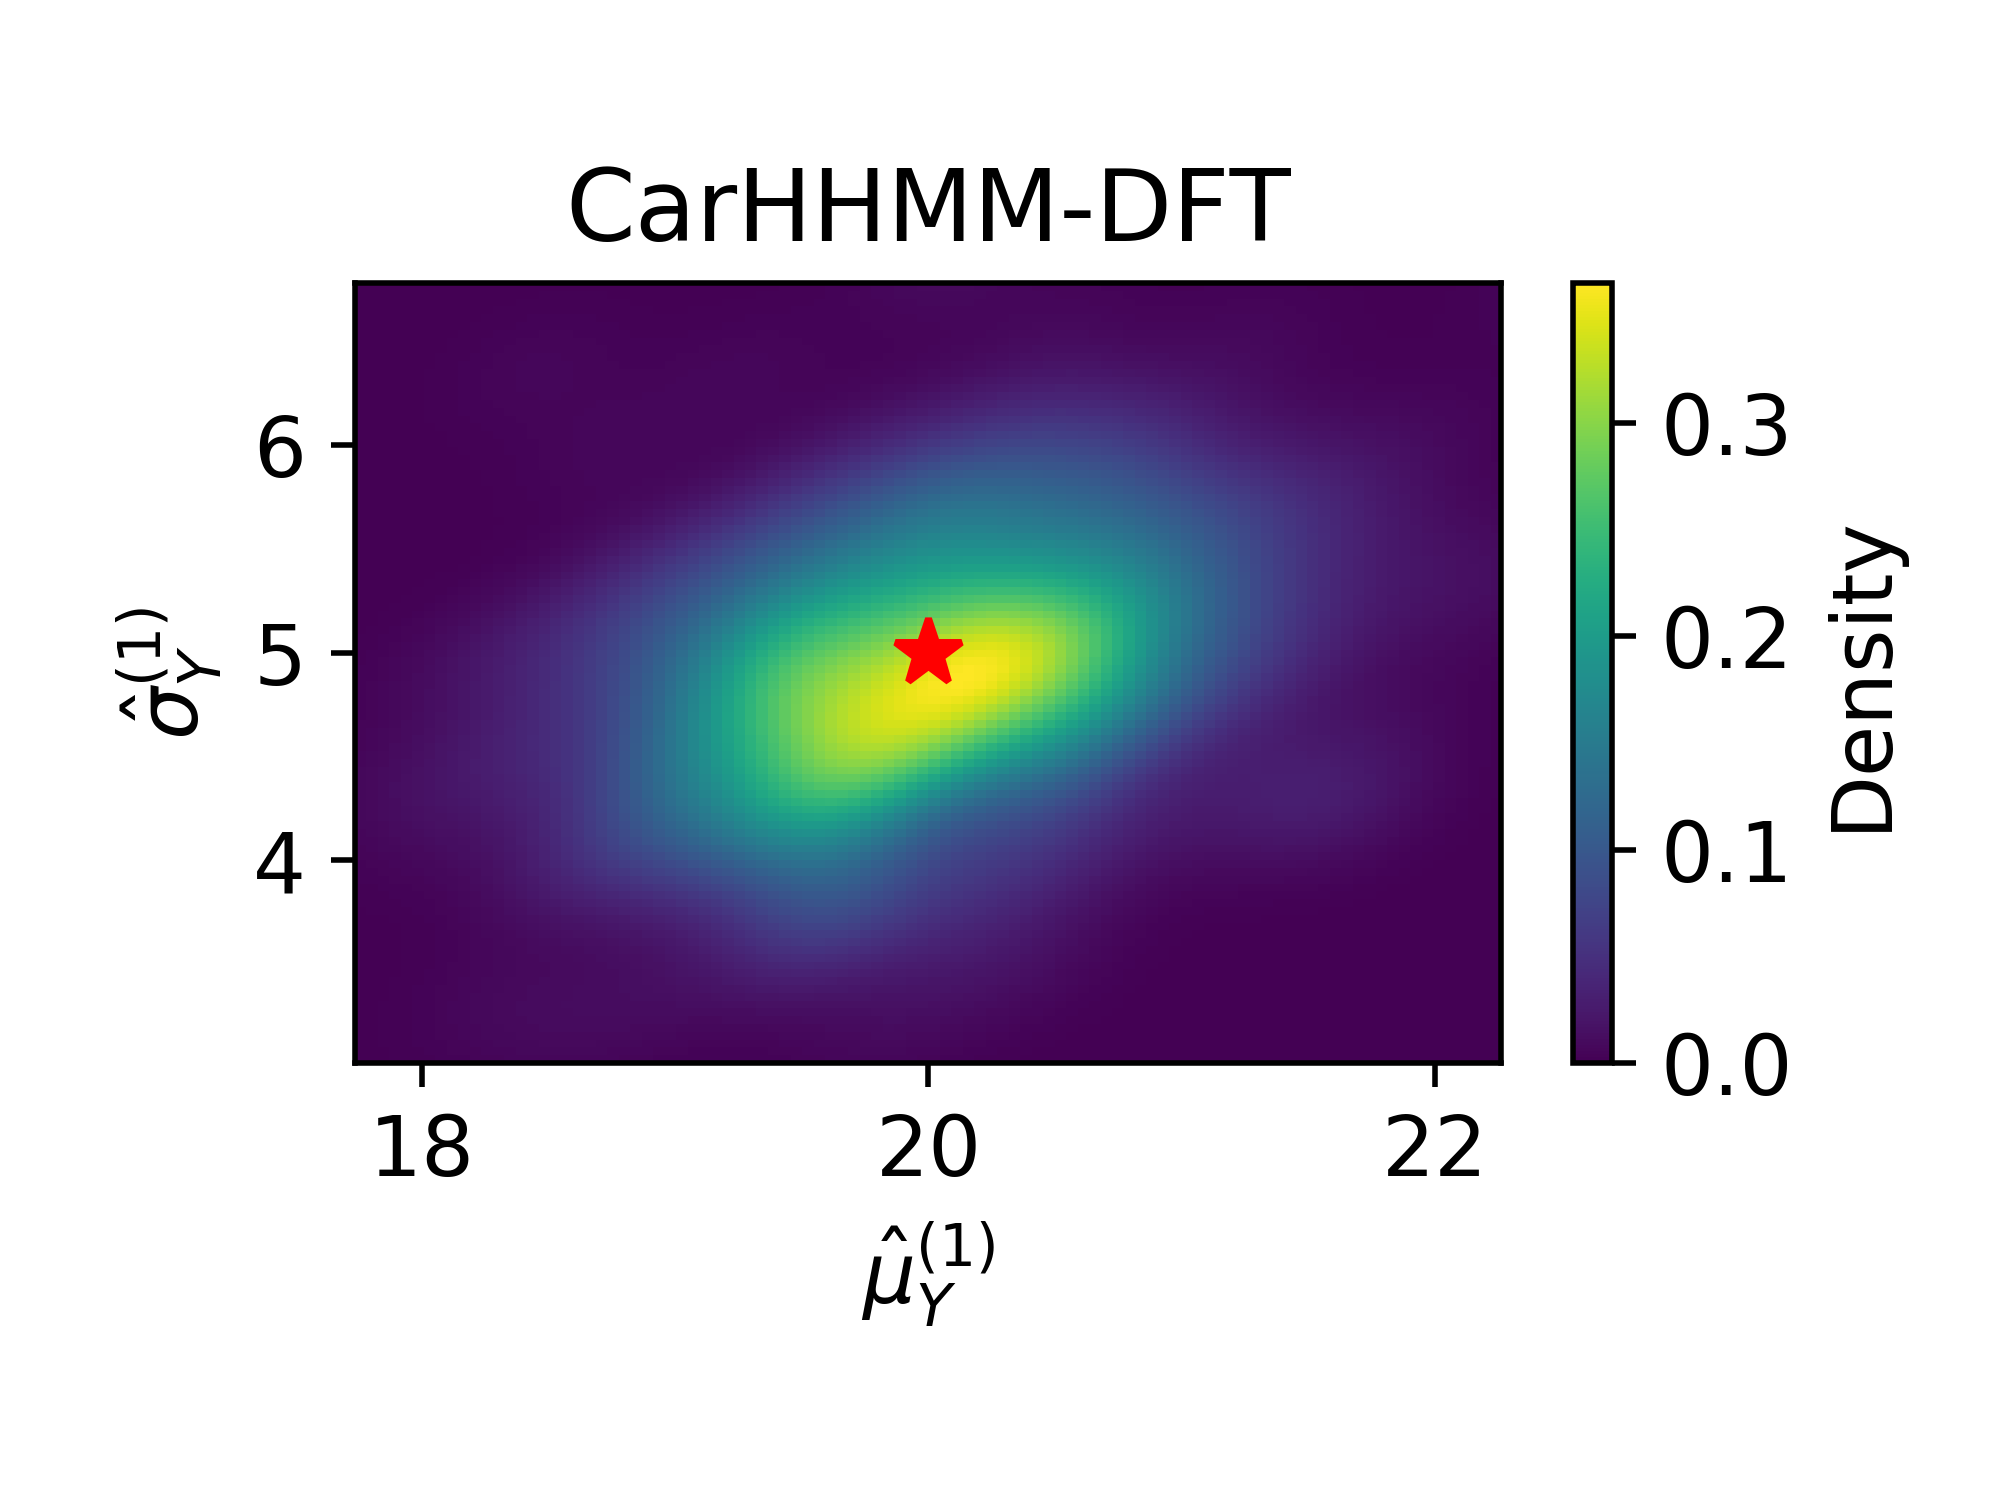
\includegraphics[width=3in]{../Plots/hhmm_FV_MLE_density_dive_duration_-1_0.png}
        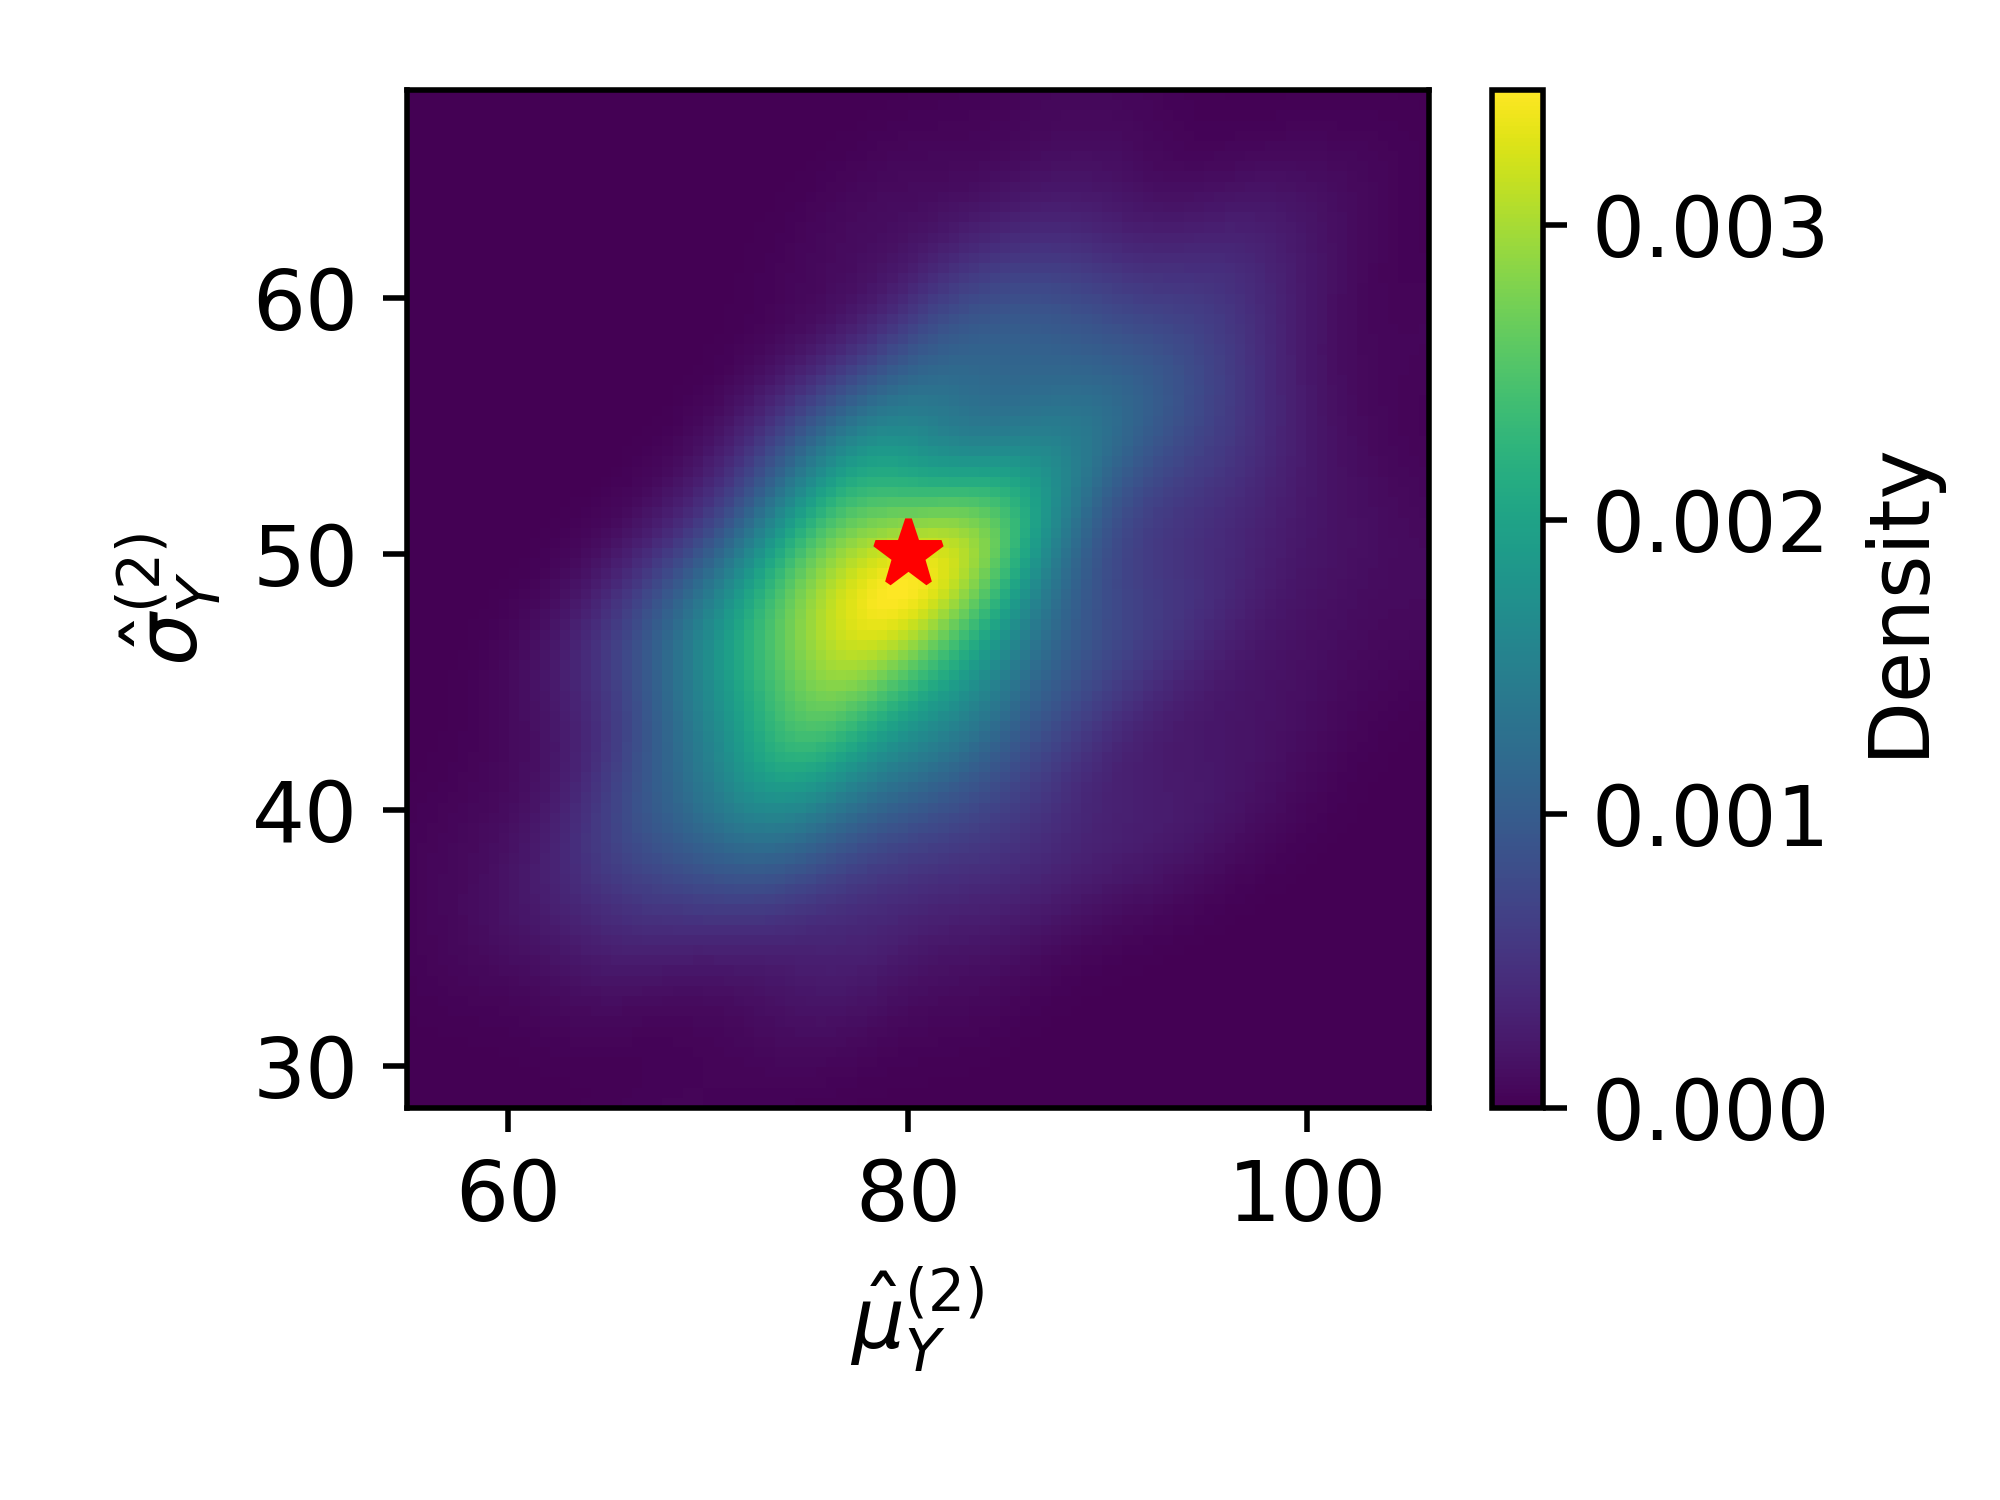
\includegraphics[width=3in]{../Plots/hhmm_FV_MLE_density_dive_duration_-1_1.png}
        \end{center}
        
        \noindent Figure \arabic{fignum}: Kernel density estimates of the distributions of estimates of dive duration parameter estimates ($\hat \mu_Y$ and $\hat \sigma_Y$). These estimates are associated with the CarHHMM-DFT and correspond to both dive types. The red star represents the true values of $\mu_Y$ and $\sigma_Y$ for both dive types.
        \addtocounter{fignum}{1}
        
        \subsection{HHMM-DFT}
        \begin{center}
        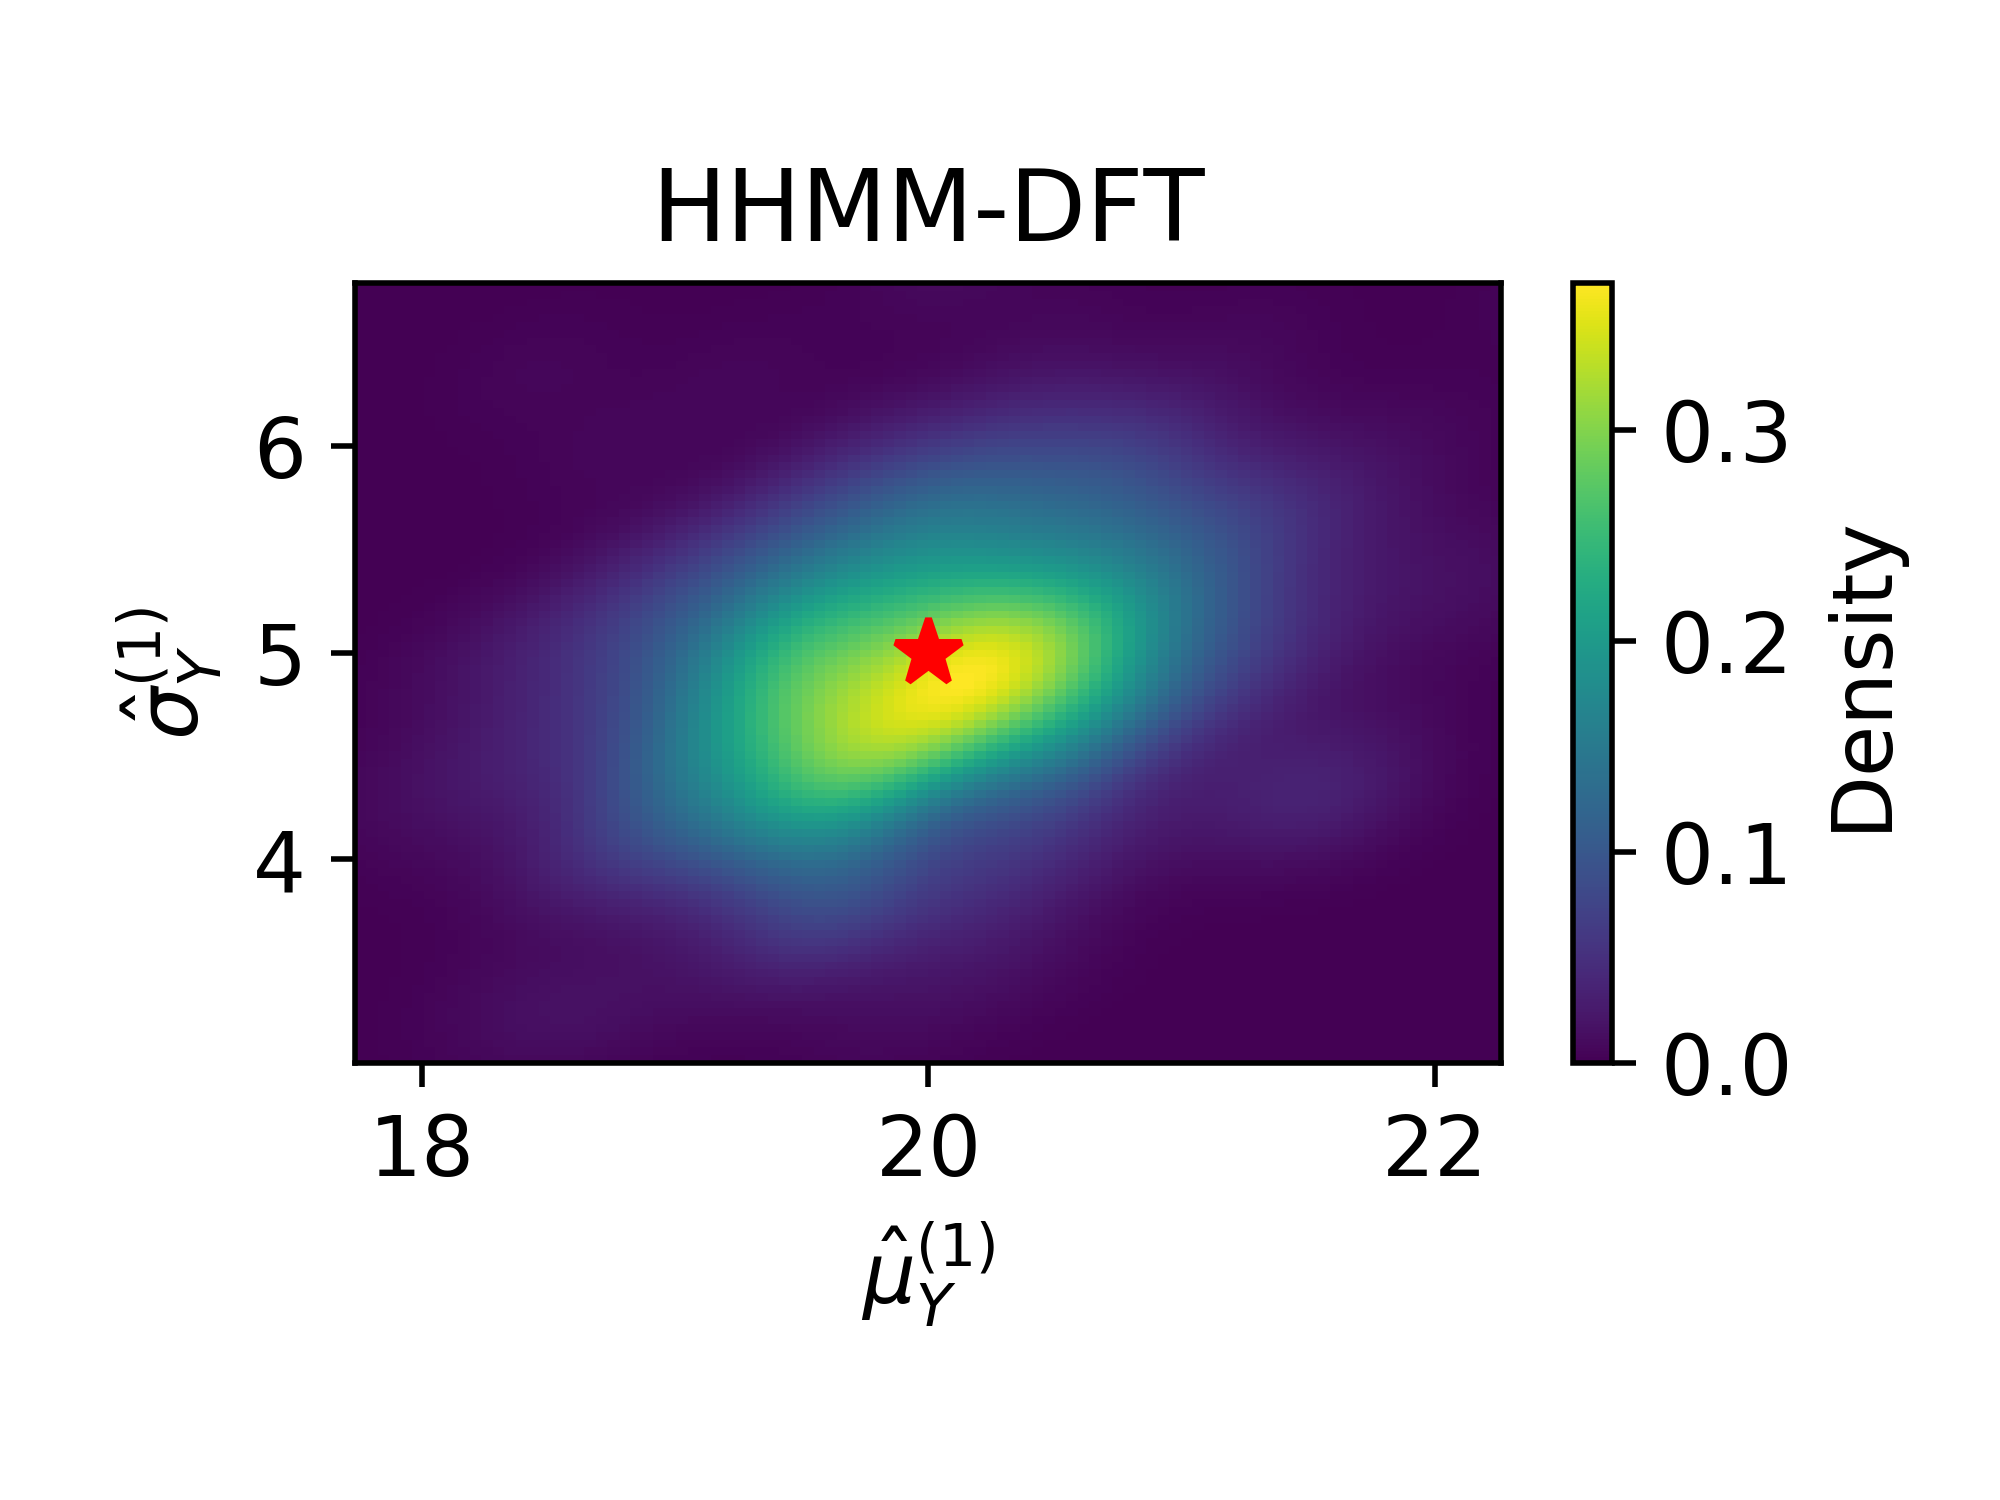
\includegraphics[width=3in]{../Plots/hhmm_FV_uncorr_MLE_density_dive_duration_-1_0.png}
        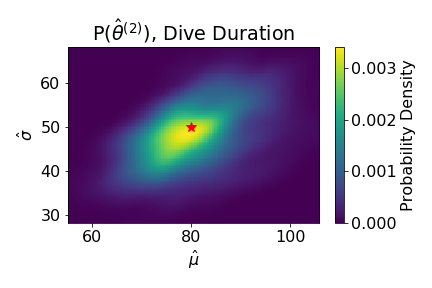
\includegraphics[width=3in]{../Plots/hhmm_FV_uncorr_MLE_density_dive_duration_-1_1.png}
        \end{center}

        \noindent Figure \arabic{fignum}: Kernel density estimate of the distributions of estimates of dive duration parameter estimates ($\hat \mu_Y$ and $\hat \sigma_Y$). These estimates are associated with the HHMM-DFT and correspond to both dive types. The red star represents the true values of $\mu_Y$ and $\sigma_Y$ for both dive types.
        \addtocounter{fignum}{1}
        
        \subsection{CarHHMM}
        \begin{center}
        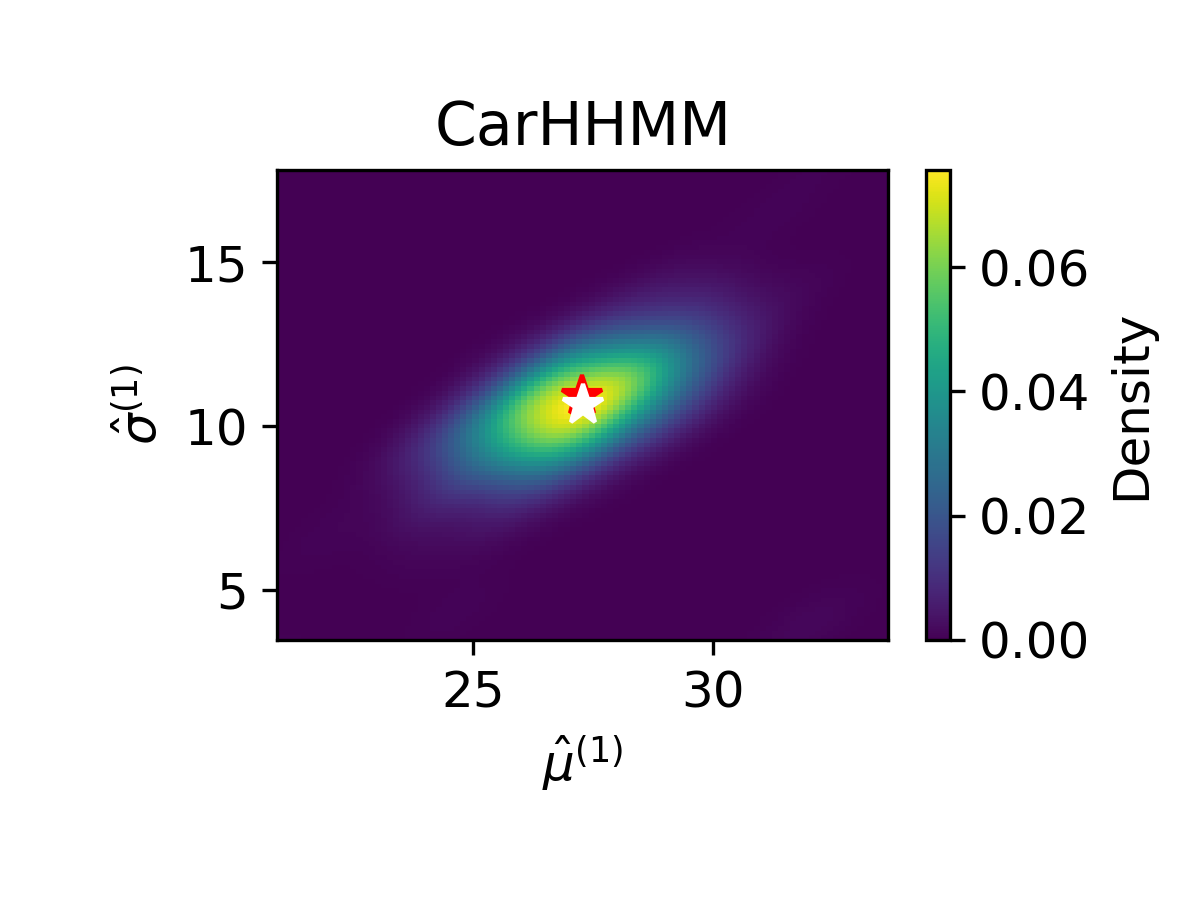
\includegraphics[width=3in]{../Plots/hhmm_V_MLE_density_dive_duration_-1_0.png}
        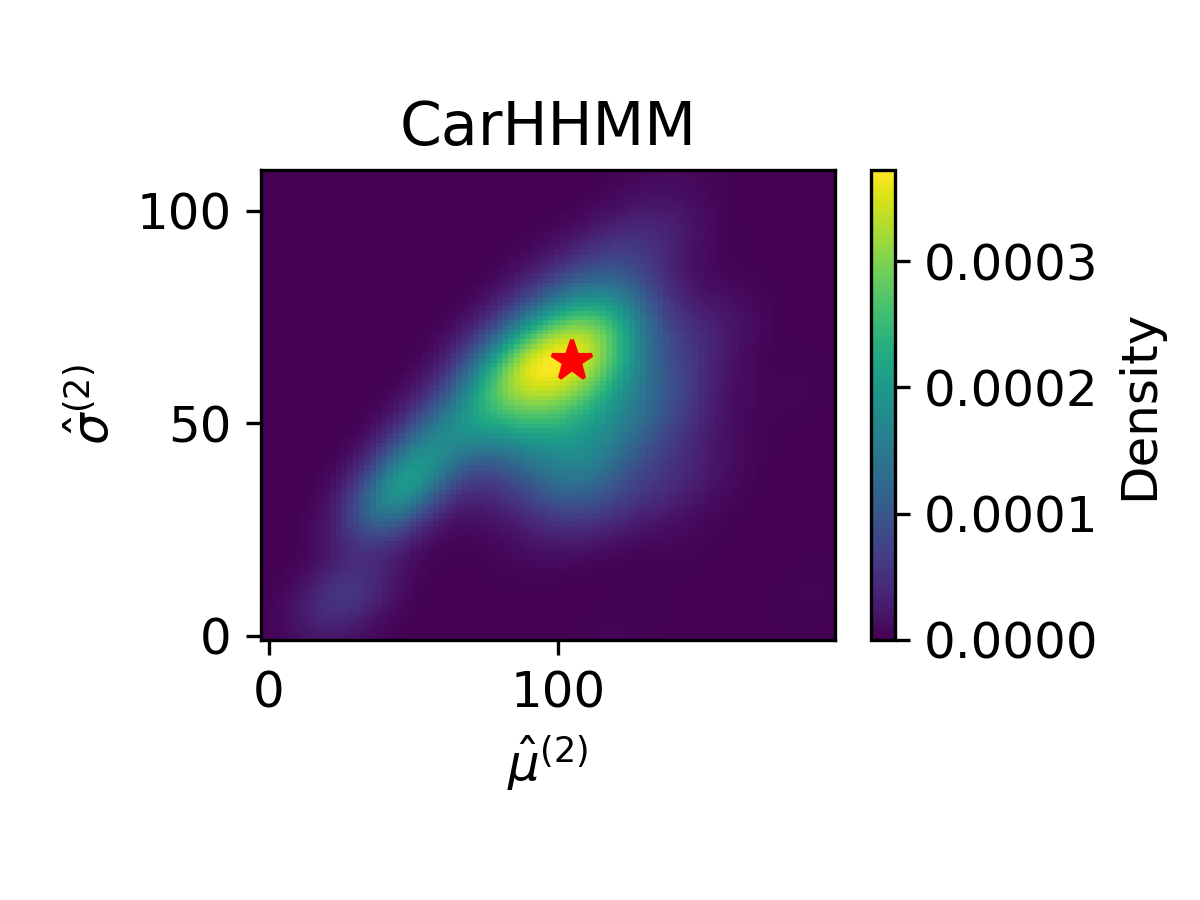
\includegraphics[width=3in]{../Plots/hhmm_V_MLE_density_dive_duration_-1_1.png}
        \end{center}
        
        \noindent Figure \arabic{fignum}: Kernel density estimate of the distributions of dive duration parameter estimates ($\hat \mu_Y$ and $\hat \sigma_Y$). These estimates are associated with the CarHHMM and correspond to both dive types. The red star represents the true values of $\mu_Y$ and $\sigma_Y$ for both dive types.
        \addtocounter{fignum}{1}
        
        \subsection{CarHMM-DFT}
        \begin{center}
        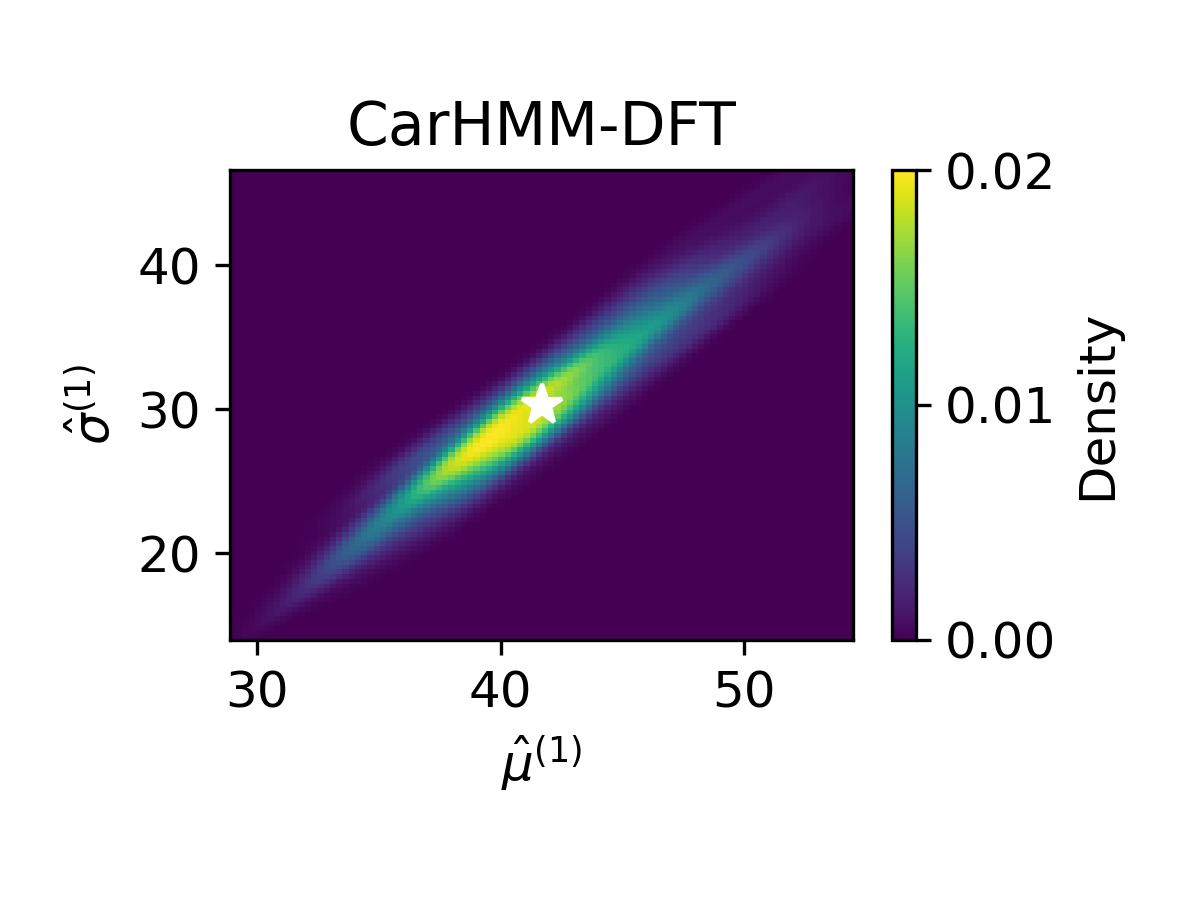
\includegraphics[width=3in]{../Plots/hmm_FV_MLE_density_dive_duration_-1_0.png}
        \end{center}
        
        \noindent Figure \arabic{fignum}: Kernel density estimate of the distributions of dive duration parameter estimates ($\hat \mu_Y$ and $\hat \sigma_Y$). These estimates are associated with the CarHMM-DFT. There is no red star which represents the true values because the CarHMM-DFT assumes that there is only one dive type.
        \addtocounter{fignum}{1}
    
    \newpage
    \section{Empirical joint distributions - acceleration ($\Zone_{t,\tilde t^*}$)}

        \begin{center}
        \scalebox{0.75}{
        \bgroup
        \centering
        \def\arraystretch{1.5}
\begin{tabular}{ccccccc}
Model                       & \multicolumn{1}{c}{Parameter} & \multicolumn{1}{c}{Subdive Type} & \multicolumn{1}{c}{Estimate}   & \multicolumn{1}{c}{Bias}   & \multicolumn{1}{c}{Empirical SE}   & \multicolumn{1}{c}{Observed Fischer SE}     \\ \hline
\multirow{9}{*}{CarHHMM-DFT}& \multirow{3}{*}{$\mu_A^*$}    & 1                                & $-0.012$                         & $-0.012$ $(p=0.004)$          & $0.093$                             & $0.066 \pm 0.038$                             \\
                            &                               & 2                                & $0.099$                         & $-0.001$ $(p=0.436)$          & $0.019$                             & $0.019 \pm 0.003$                             \\
                            &                               & 3                                & $0.200$                         & $0.000$ $(p=0.965)$          & $0.060$                             & $0.053 \pm 0.013$                             \\
                            & \multirow{3}{*}{$\sigma_A^*$} & 1                                & $0.050$                         & $0.000$ $(p=0.376)$          & $0.002$                             & $0.002 \pm 0.000$                             \\
                            &                               & 2                                & $0.100$                         & $-0.000$ $(p=0.672)$          & $0.002$                             & $0.002 \pm 0.000$                             \\ 
                            &                               & 3                                & $0.298$                         & $-0.002$ $(p=0.024)$          & $0.016$                             & $0.015 \pm 0.002$                             \\
                            & \multirow{3}{*}{$\phi_A^*$}   & 1                                & $0.968$                         & $-0.002$ $(p=0.001)$          & $0.012$                             & $0.010 \pm 0.002$                             \\
                            &                               & 2                                & $0.828$                         & $-0.002$ $(p=0.007)$          & $0.017$                             & $0.017 \pm 0.002$                             \\
                            &                               & 3                                & $0.600$                         & $-0.010$ $(p=0.001)$          & $0.064$                             & $0.065 \pm 0.011$                             \\ \hline
\multirow{9}{*}{HHMM-DFT}   & \multirow{3}{*}{$\mu_A^*$}    & 1                                & $0.048$                         & $0.048$ $(p=0.000)$          & $0.033$                             & $0.007 \pm 0.001$                             \\
                            &                               & 2                                & $0.087$                         & $-0.013$ $(p=0.000)$          & $0.018$                             & $0.006 \pm 0.001$                             \\
                            &                               & 3                                & $0.215$                         & $0.015$ $(p=0.000)$          & $0.065$                             & $0.022 \pm 0.004$                             \\
                            & \multirow{3}{*}{$\sigma_A^*$} & 1                                & $0.160$                         & $0.110$ $(p=0.000)$          & $0.023$                             & $0.005 \pm 0.001$                             \\
                            &                               & 2                                & $0.158$                         & $0.058$ $(p=0.000)$          & $0.010$                             & $0.004 \pm 0.000$                             \\ 
                            &                               & 3                                & $0.356$                         & $0.056$ $(p=0.000)$          & $0.035$                             & $0.015 \pm 0.002$                             \\
                            & \multirow{3}{*}{$\phi_A^*$}   & 1                                & ------                         & ------                     & ------                             & ------                                      \\
                            &                               & 2                                & ------                         & ------                     & ------                             & ------                                      \\
                            &                               & 3                                & ------                         & ------                     & ------                             & ------                                      \\ \hline
\multirow{9}{*}{CarHHMM}    & \multirow{3}{*}{$\mu_A^*$}    & 1                                & $0.060$                         & $0.060$ $(p=0.000)$          & $0.034$                             & $0.024 \pm 0.054$                             \\
                            &                               & 2                                & $0.097$                         & $-0.003$ $(p=0.000)$          & $0.016$                             & $0.052 \pm 0.055$                             \\
                            &                               & 3                                & $0.201$                         & $0.001$ $(p=0.634)$          & $0.058$                             & $0.018 \pm 0.007$                             \\
                            & \multirow{3}{*}{$\sigma_A^*$} & 1                                & $0.111$                         & $0.061$ $(p=0.000)$          & $0.004$                             & $0.006 \pm 0.042$                             \\
                            &                               & 2                                & $0.285$                         & $0.185$ $(p=0.000)$          & $0.009$                             & $0.040 \pm 0.043$                             \\ 
                            &                               & 3                                & $1.150$                         & $0.850$ $(p=0.000)$          & $0.080$                             & $0.003 \pm 0.001$                             \\
                            & \multirow{3}{*}{$\phi_A^*$}   & 1                                & $0.830$                         & $-0.140$ $(p=0.000)$          & $0.048$                             & $0.016  $                             \\
                            &                               & 2                                & $0.004$                         & $-0.826$ $(p=0.000)$          & $0.012$                             & $0.023  $                             \\
                            &                               & 3                                & $0.000$                         & $-0.610$ $(p=0.000)$          & $0.000$                             & $0.016 \pm 0.004$                             \\ \hline
\multirow{9}{*}{CarHMM-DFT} & \multirow{3}{*}{$\mu_A^*$}    & 1                                & $-0.008$                         & $-0.008$ $(p=0.142)$          & $0.114$                             & $0.064 \pm 0.037$                             \\
                            &                               & 2                                & $0.101$                         & $0.001$ $(p=0.438)$          & $0.019$                             & $0.019 \pm 0.003$                             \\
                            &                               & 3                                & $0.200$                         & $0.000$ $(p=0.926)$          & $0.057$                             & $0.054 \pm 0.014$                             \\
                            & \multirow{3}{*}{$\sigma_A^*$} & 1                                & $0.050$                         & $-0.000$ $(p=0.005)$          & $0.001$                             & $0.002 \pm 0.000$                             \\
                            &                               & 2                                & $0.100$                         & $-0.000$ $(p=0.000)$          & $0.002$                             & $0.002 \pm 0.000$                             \\ 
                            &                               & 3                                & $0.299$                         & $-0.001$ $(p=0.117)$          & $0.015$                             & $0.015 \pm 0.002$                             \\
                            & \multirow{3}{*}{$\phi_A^*$}   & 1                                & $0.968$                         & $-0.002$ $(p=0.001)$          & $0.012$                             & $0.010 \pm 0.002$                             \\
                            &                               & 2                                & $0.830$                         & $-0.000$ $(p=0.552)$          & $0.016$                             & $0.017 \pm 0.002$                             \\
                            &                               & 3                                & $0.595$                         & $-0.015$ $(p=0.000)$          & $0.071$                             & $0.065 \pm 0.010$                             \\ \hline
\end{tabular}
        \egroup
        }
        \end{center}
        
        \noindent Table \arabic{tablenum}: Estimates and standard errors for the parameters of the distribution of acceleration across all four models in the simulation study. The ``Estimate" column is the average across 500 simulations, and the ``Observed Fisher SE" column is the median across 500 simulations. The $\pm$ refers to the inter-quartile range. SE stands for standard error. Reported $p$-values test if the observed bias is statistically significant using a one-sample $t$-test.
        \addtocounter{tablenum}{1}
        
        \newpage
    
        \subsection{CarHHMM-DFT}
        \begin{center}
        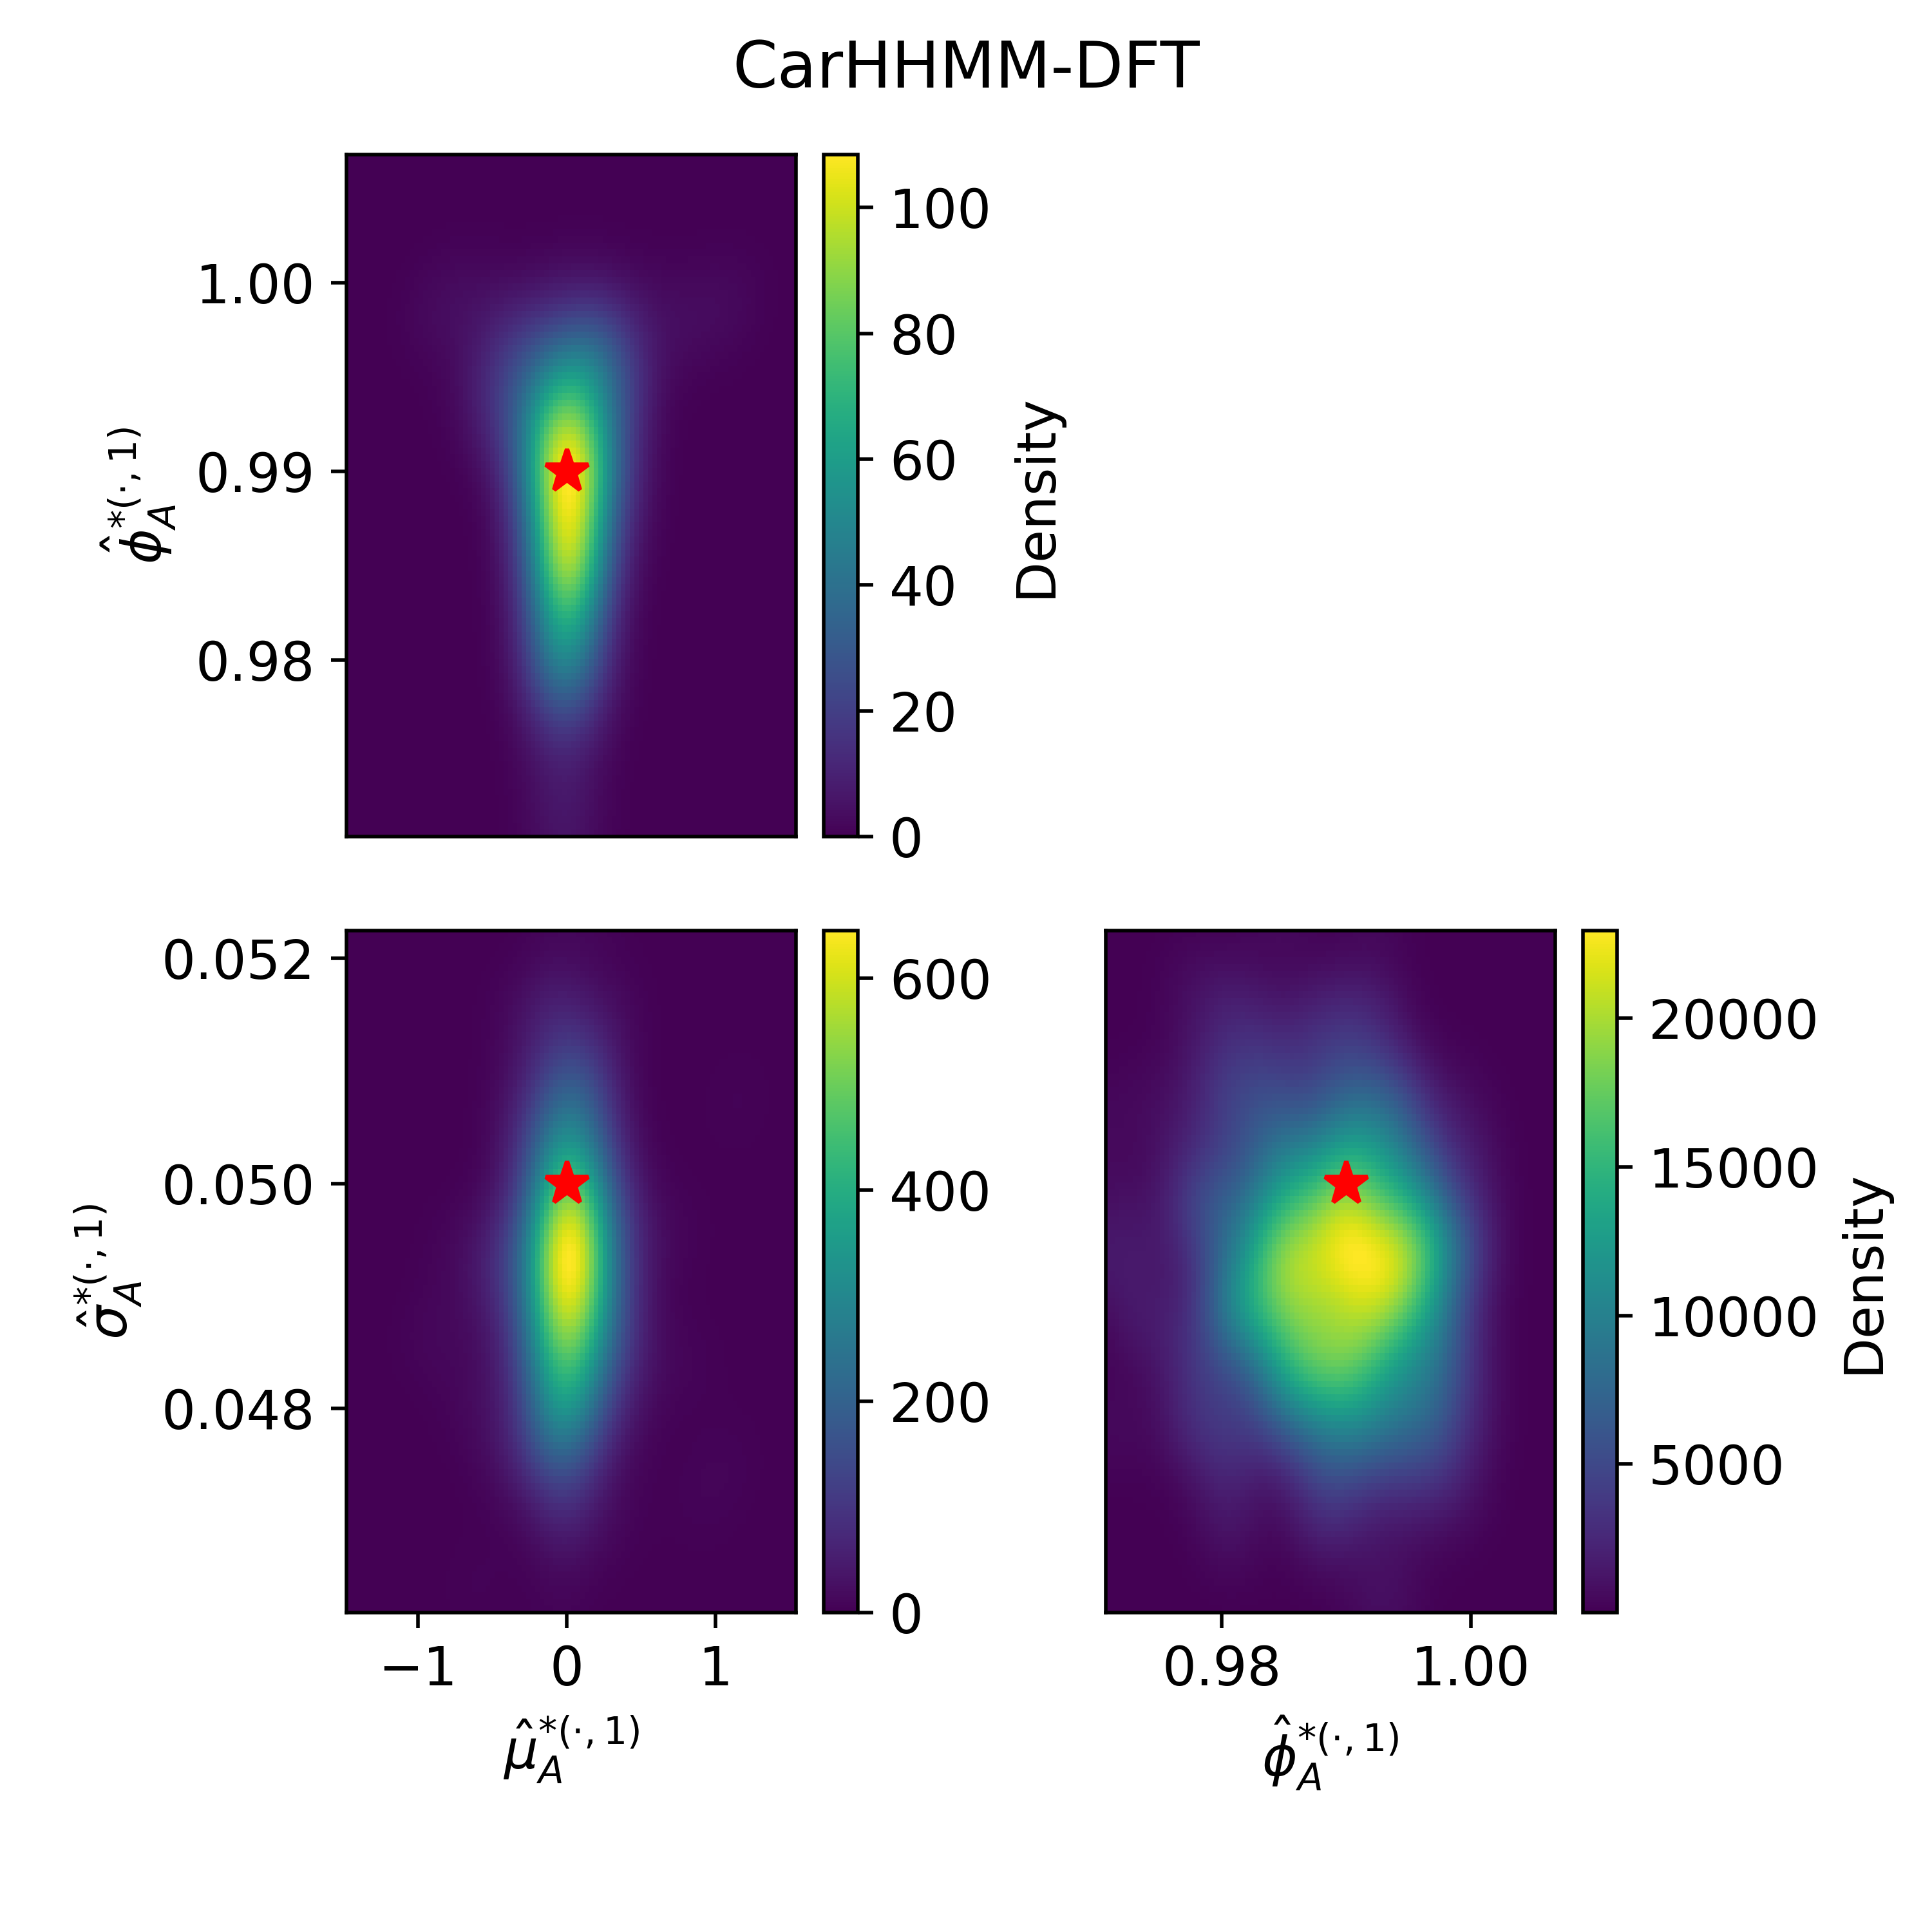
\includegraphics[width=2.1in]{../Plots/hhmm_FV_MLE_density_A_0_0.png}
        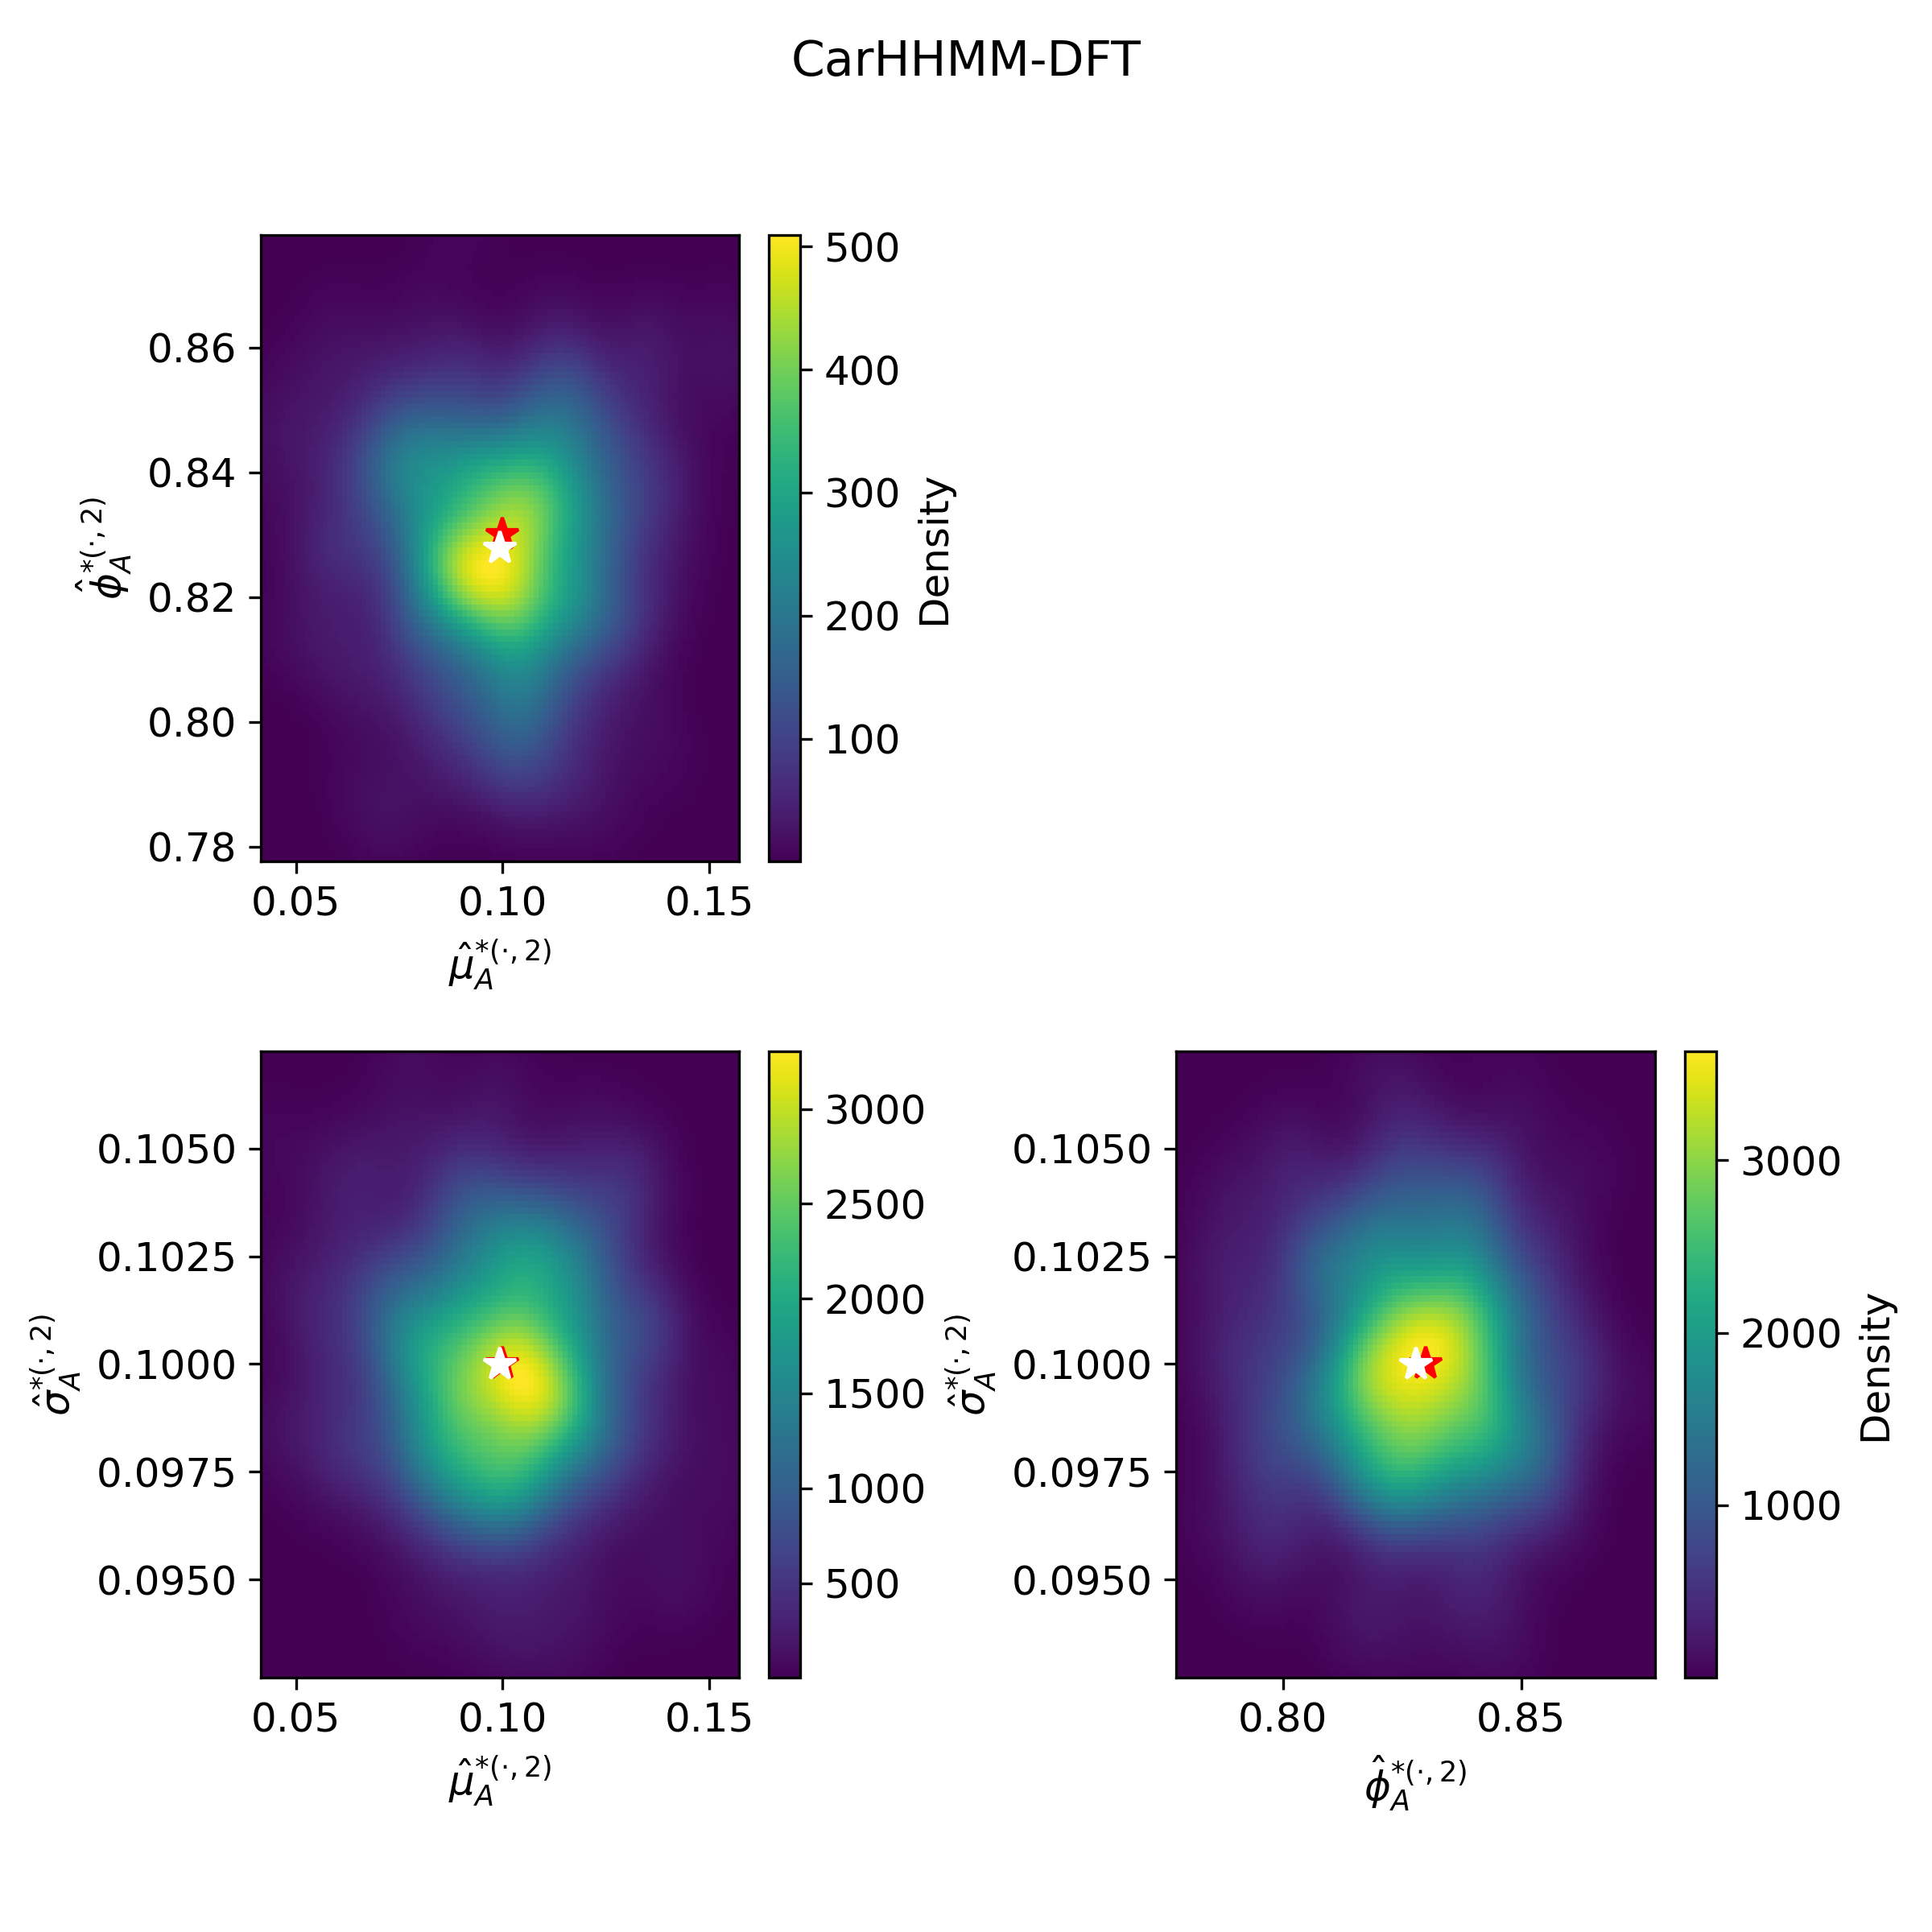
\includegraphics[width=2.1in]{../Plots/hhmm_FV_MLE_density_A_0_1.png}
        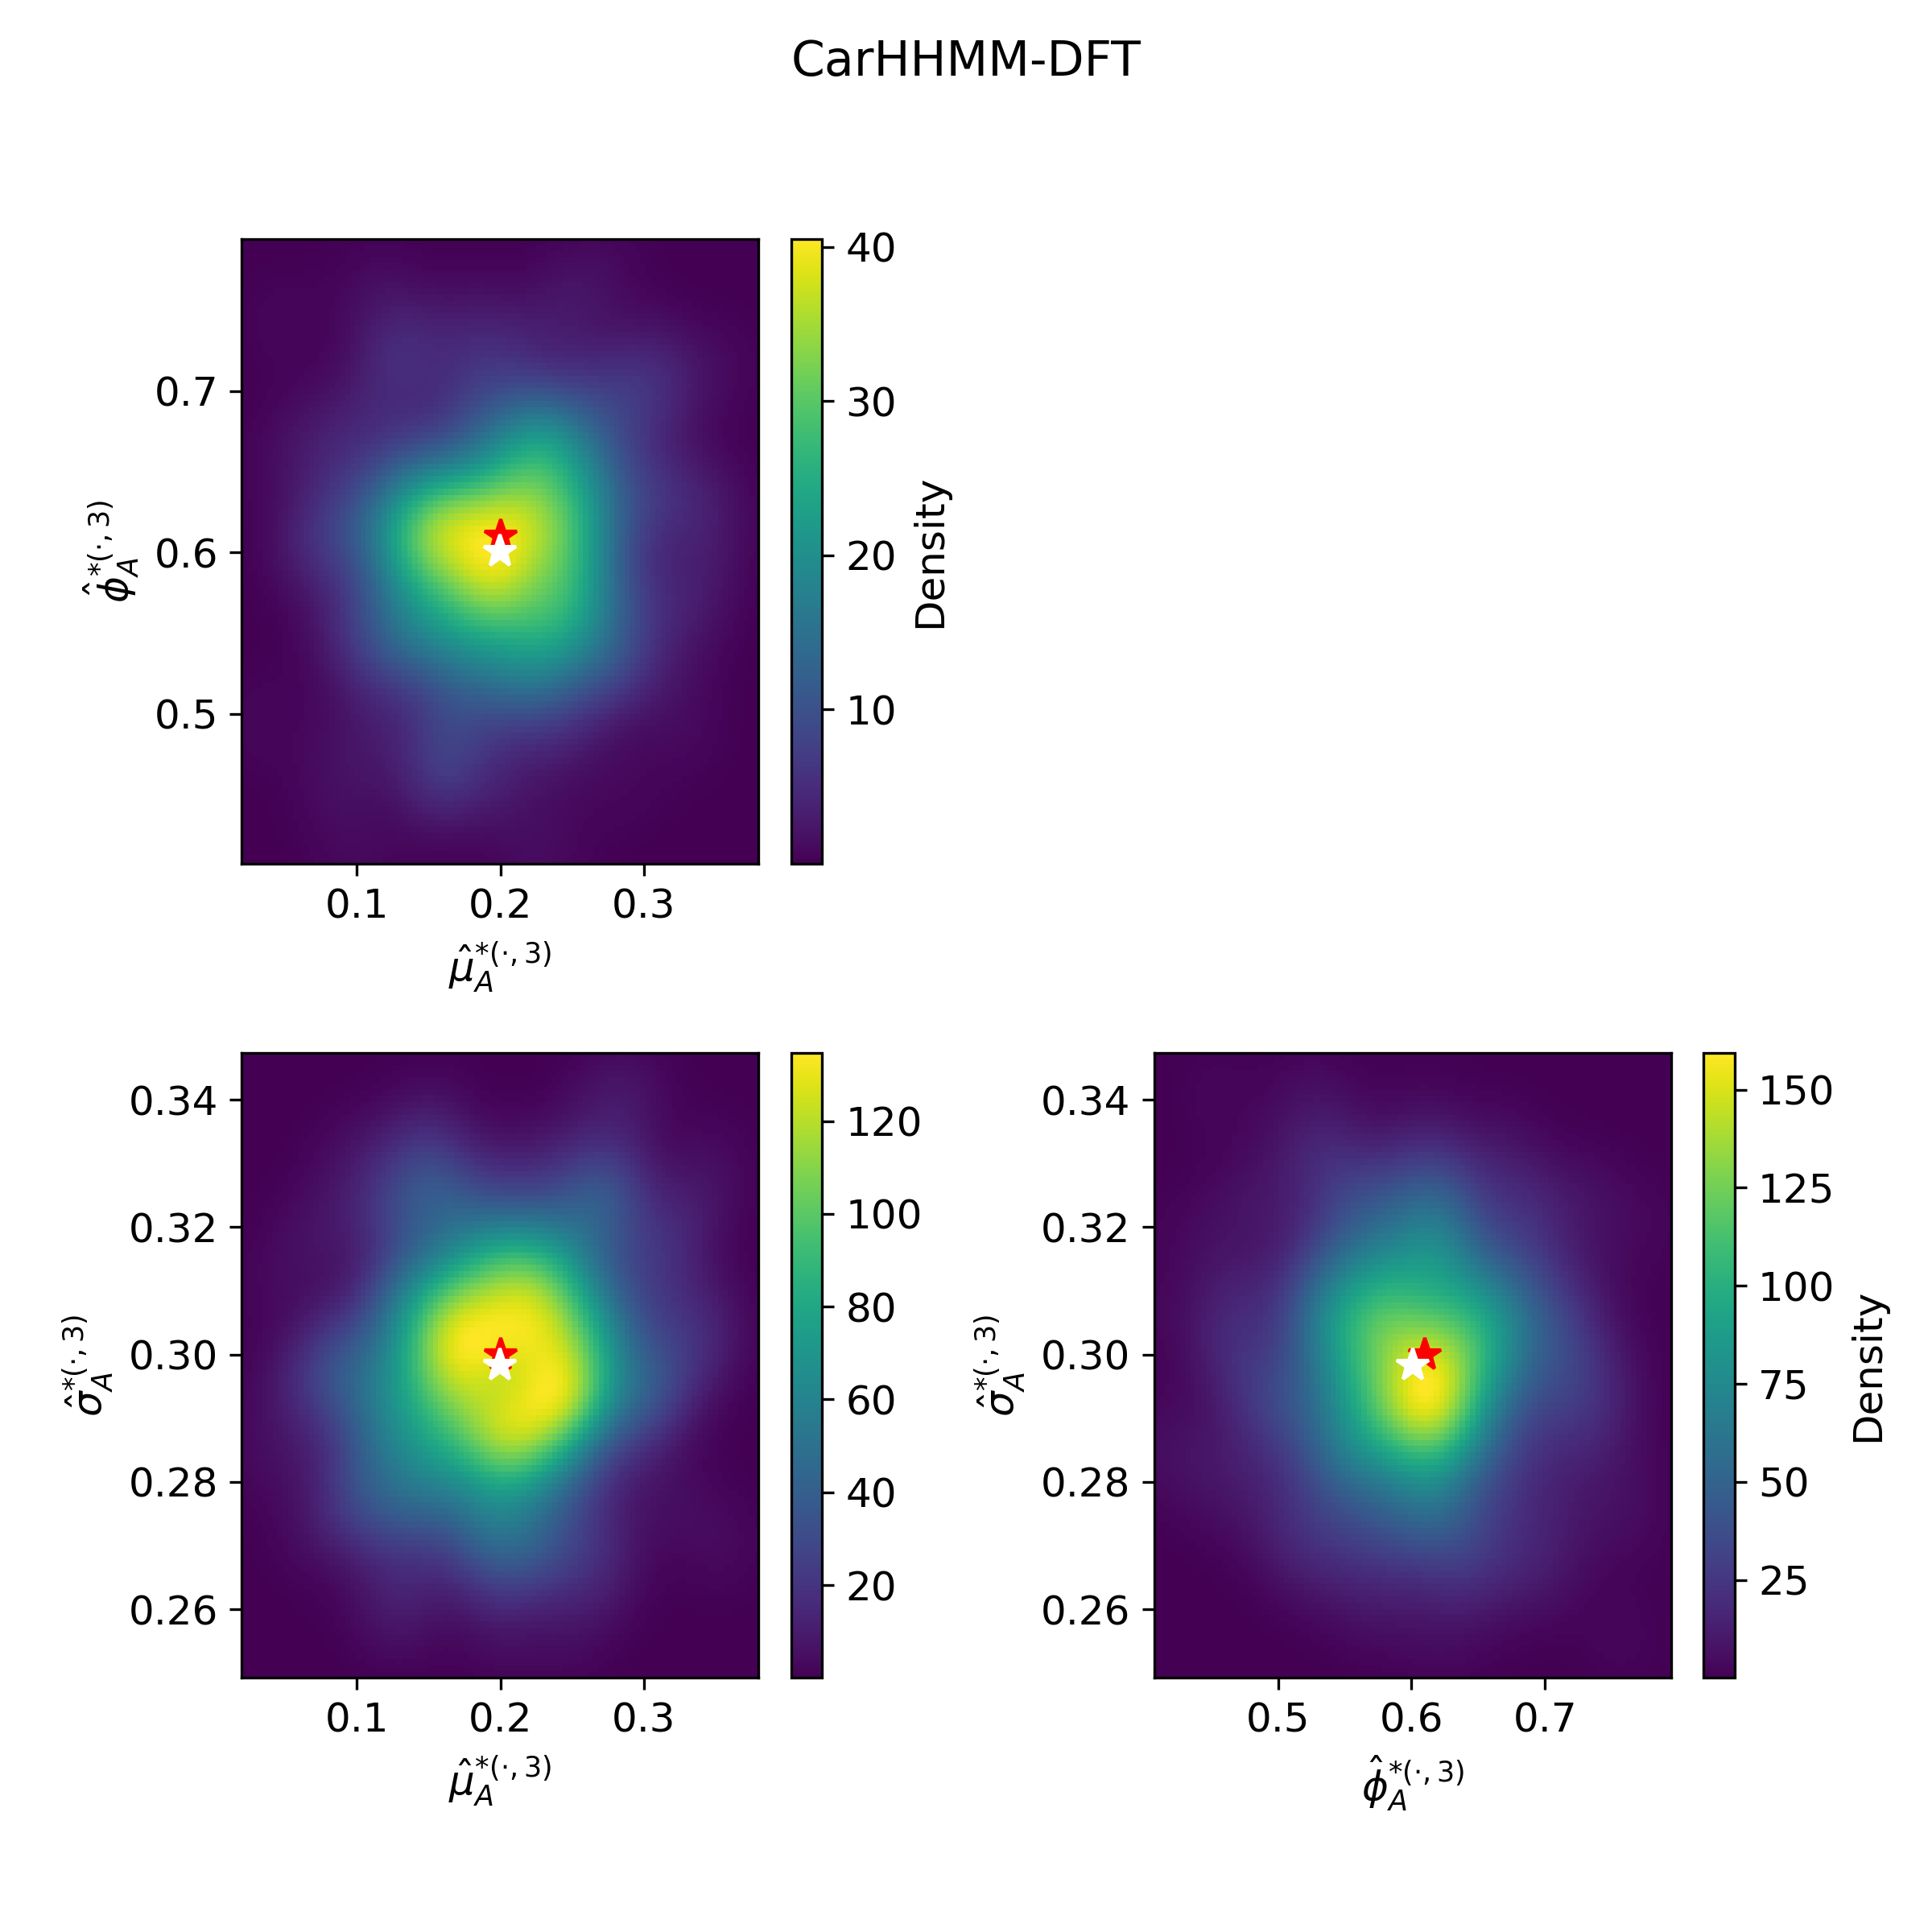
\includegraphics[width=2.1in]{../Plots/hhmm_FV_MLE_density_A_0_2.png}
        \end{center}
        
        \noindent Figure \arabic{fignum}: Kernel density estimate of the distributions of estimates of acceleration parameters ($\hat \mu^*_A$, $\hat \sigma^*_A$, and $\hat \phi^*_A$) for each subdive state. The red star represents the true values of $\mu^*_A$, $\sigma^*_A$, and $\phi^*_A$ for both subdive states. These estimates are for the CarHHMM-DFT.
        \addtocounter{fignum}{1}
        
        \subsection{HHMM-DFT}
        \begin{center}
        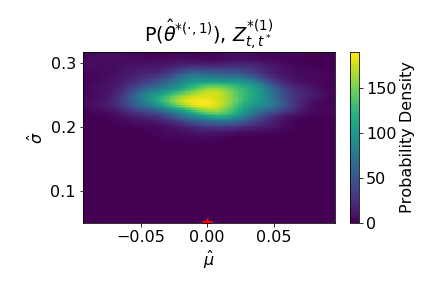
\includegraphics[width=2.1in]{../Plots/hhmm_FV_uncorr_MLE_density_A_0_0.png}
        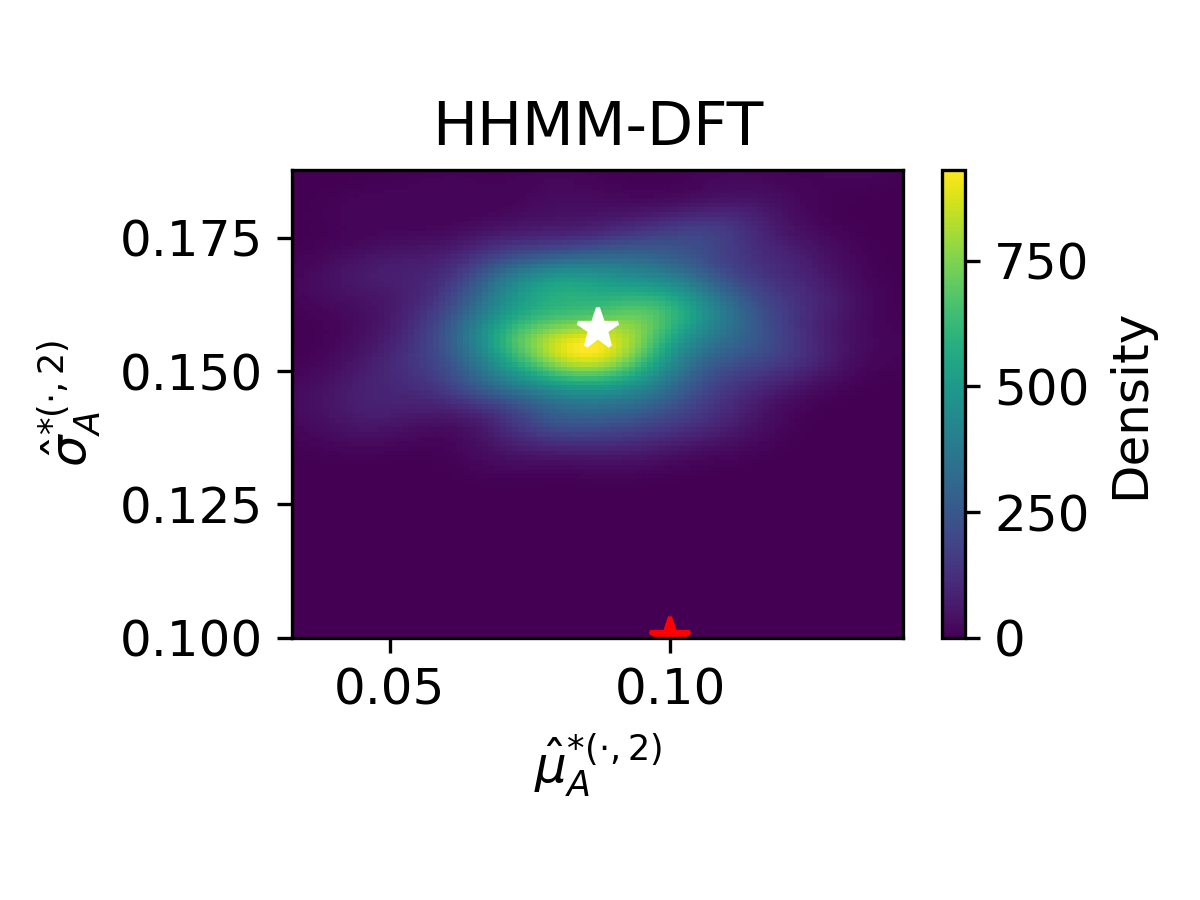
\includegraphics[width=2.1in]{../Plots/hhmm_FV_uncorr_MLE_density_A_0_1.png}
        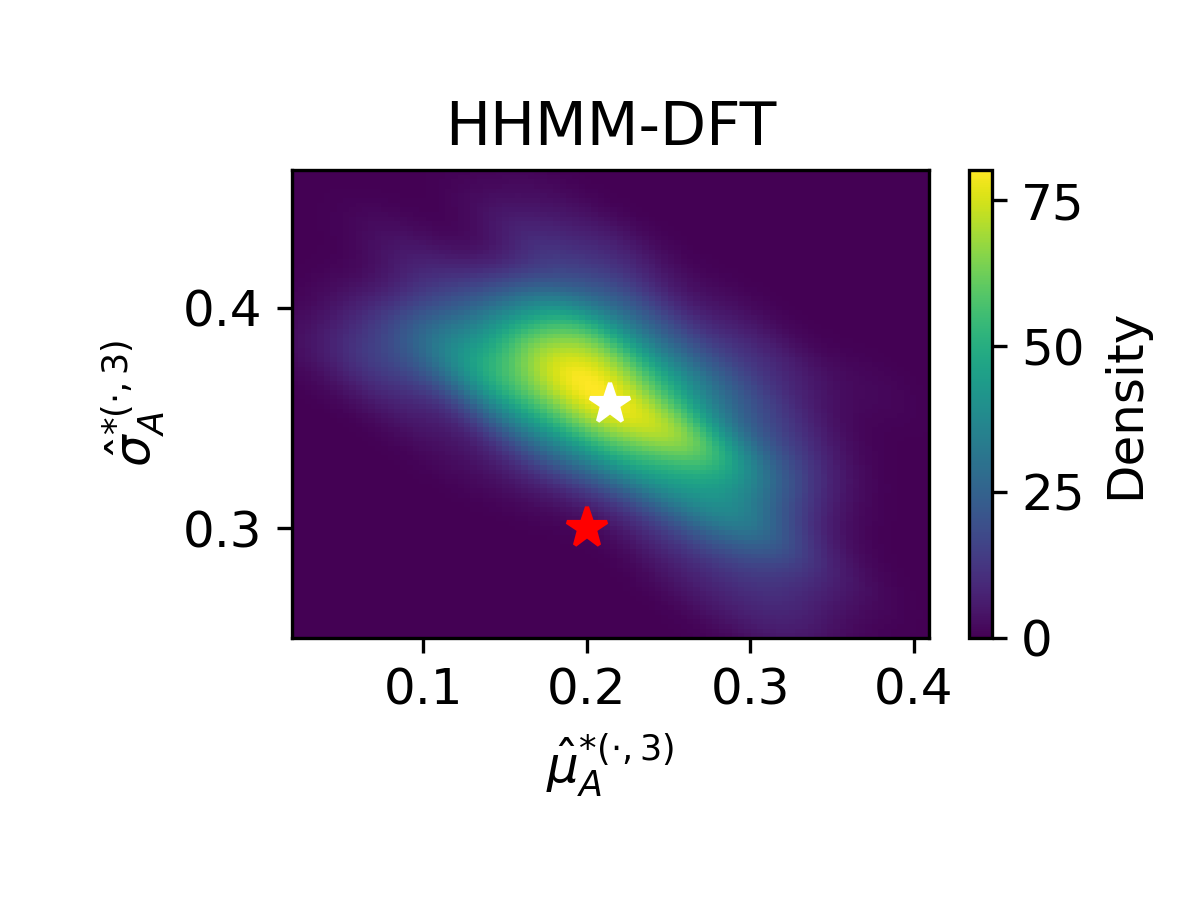
\includegraphics[width=2.1in]{../Plots/hhmm_FV_uncorr_MLE_density_A_0_2.png}
        \end{center}
        
        \noindent Figure \arabic{fignum}: Kernel density estimate of the distributions of estimates of acceleration parameters ($\hat \mu^*_A$ and $\hat \sigma^*_A$) for each subdive state. The red star represents the true values of $\mu^*_A$ and $\sigma^*_A$ for both subdive states. These estimates are for the HHMM-DFT. Note that the HHMM-DFT assumes no auto-correlation in $\Zone_{t,\tilde t^*}$, so $\hat \phi_A^{*(\cdot,i^*)}$ is absent from these plots.
        \addtocounter{fignum}{1}
        
        \subsection{CarHHMM}
        \begin{center}
        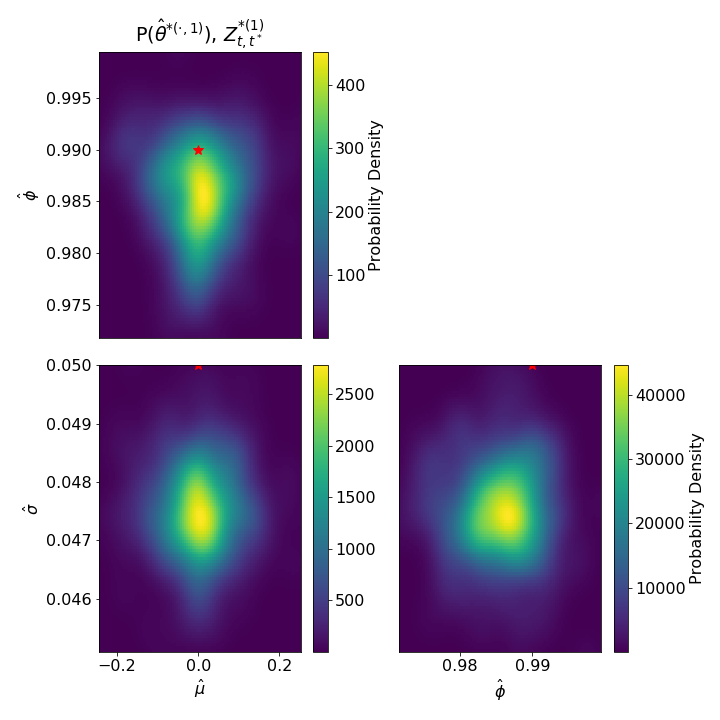
\includegraphics[width=2.1in]{../Plots/hhmm_V_MLE_density_A_0_0.png}
        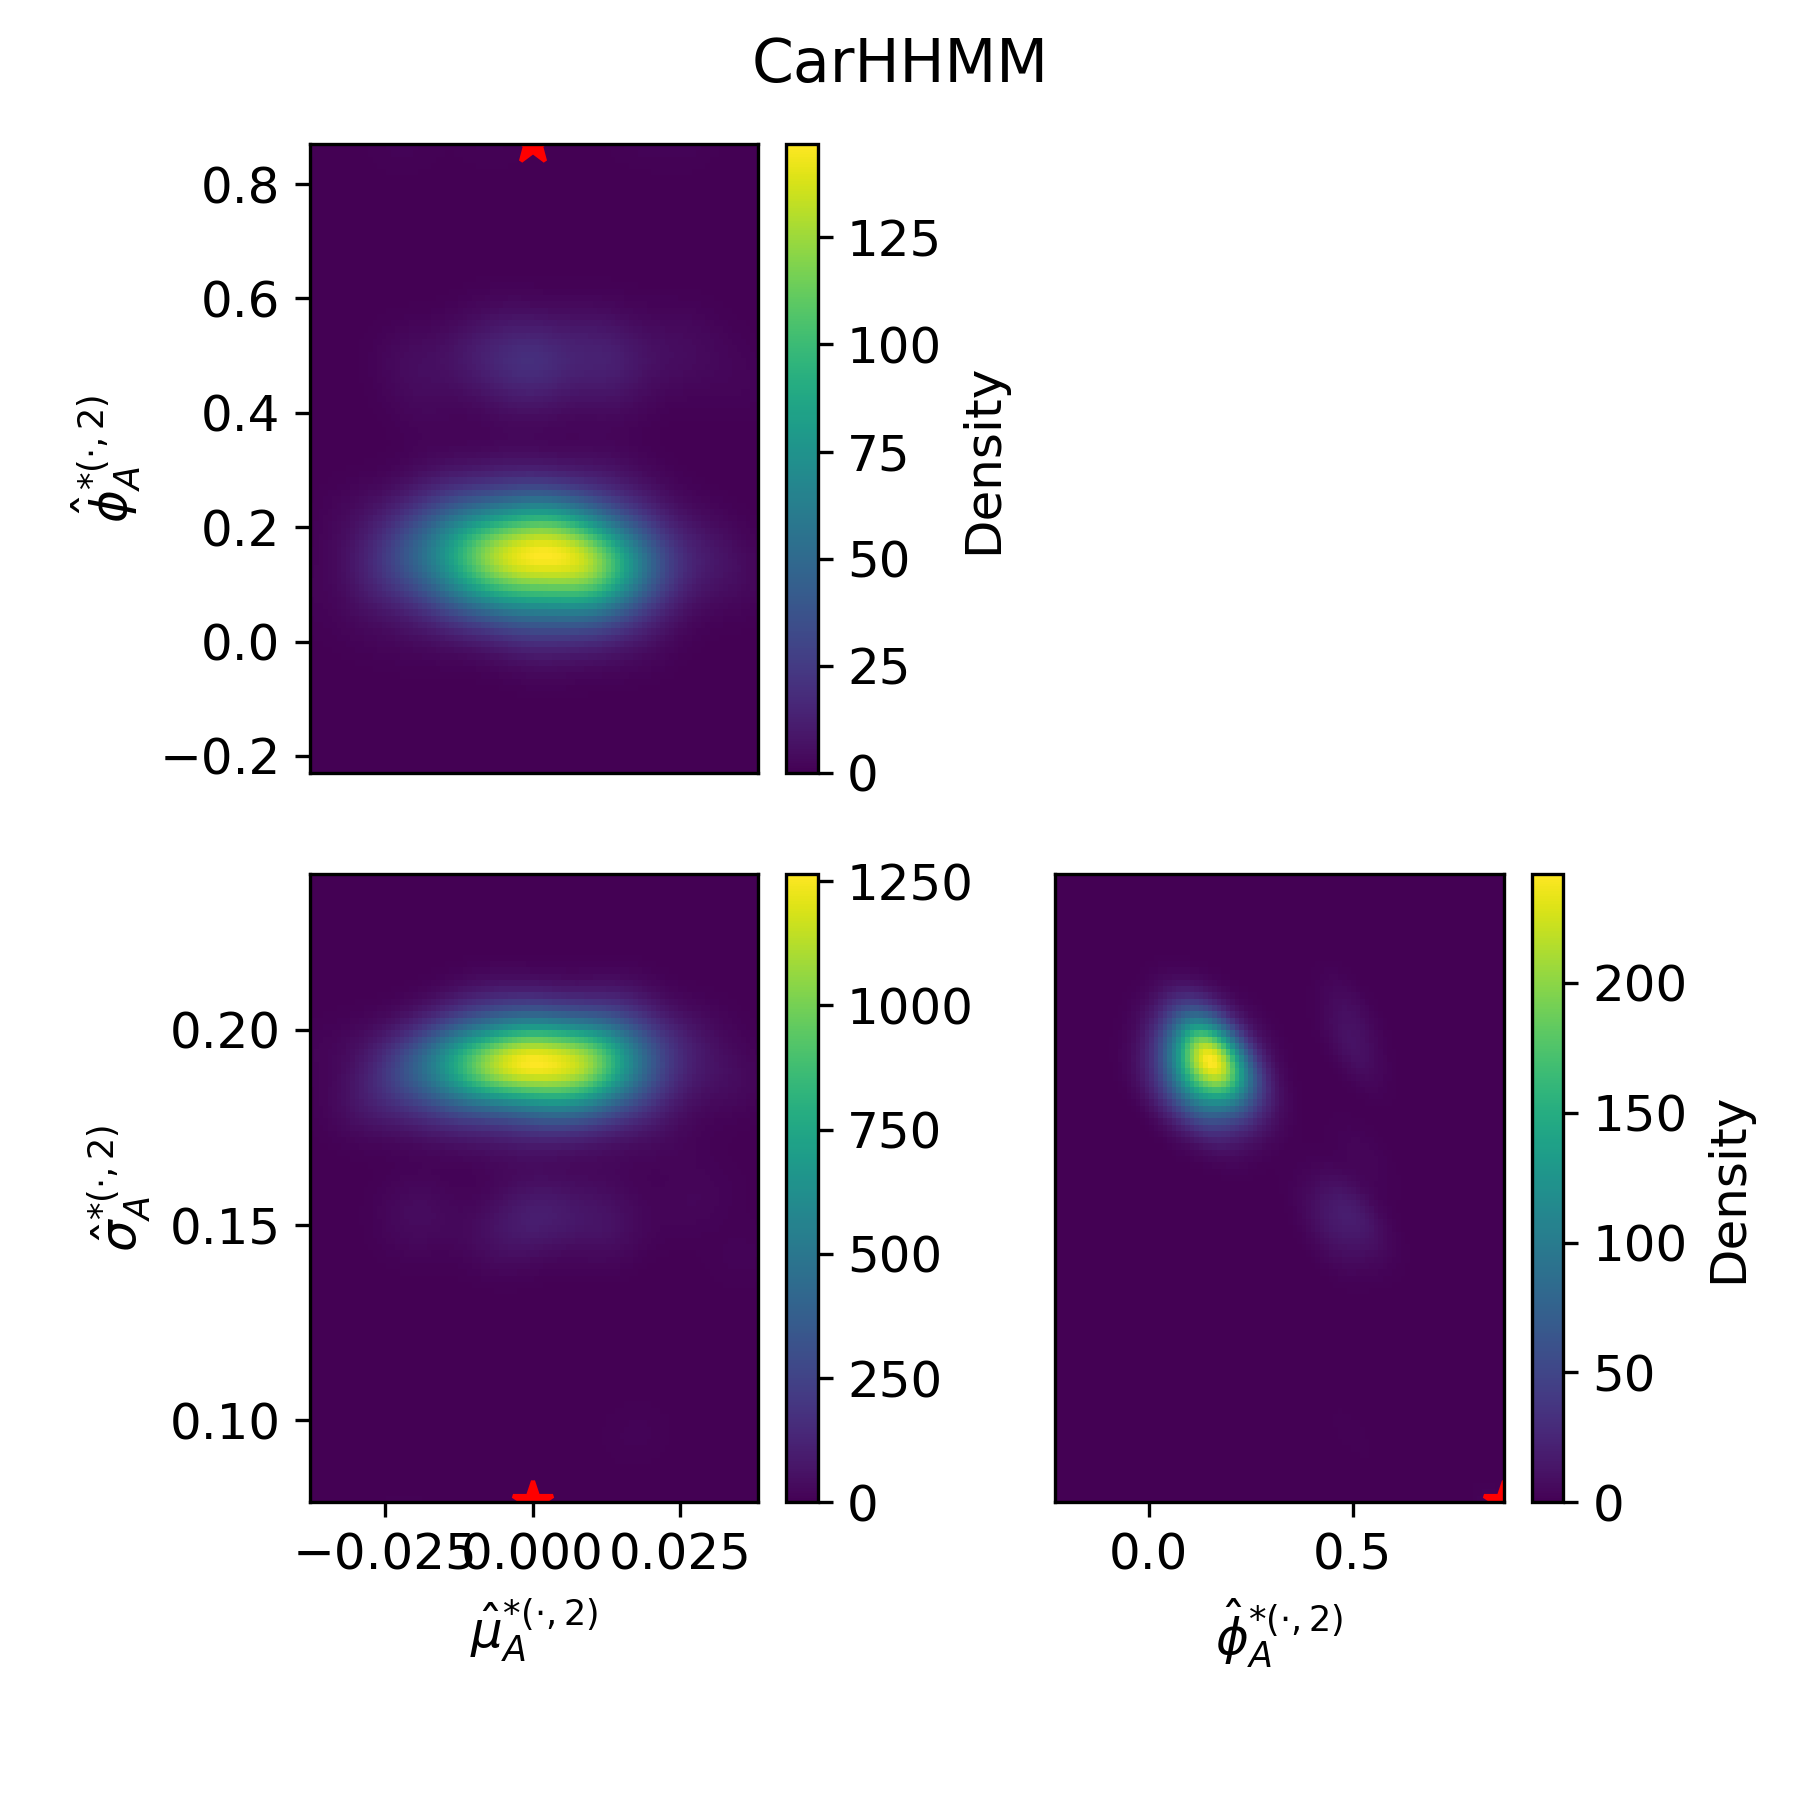
\includegraphics[width=2.1in]{../Plots/hhmm_V_MLE_density_A_0_1.png}
        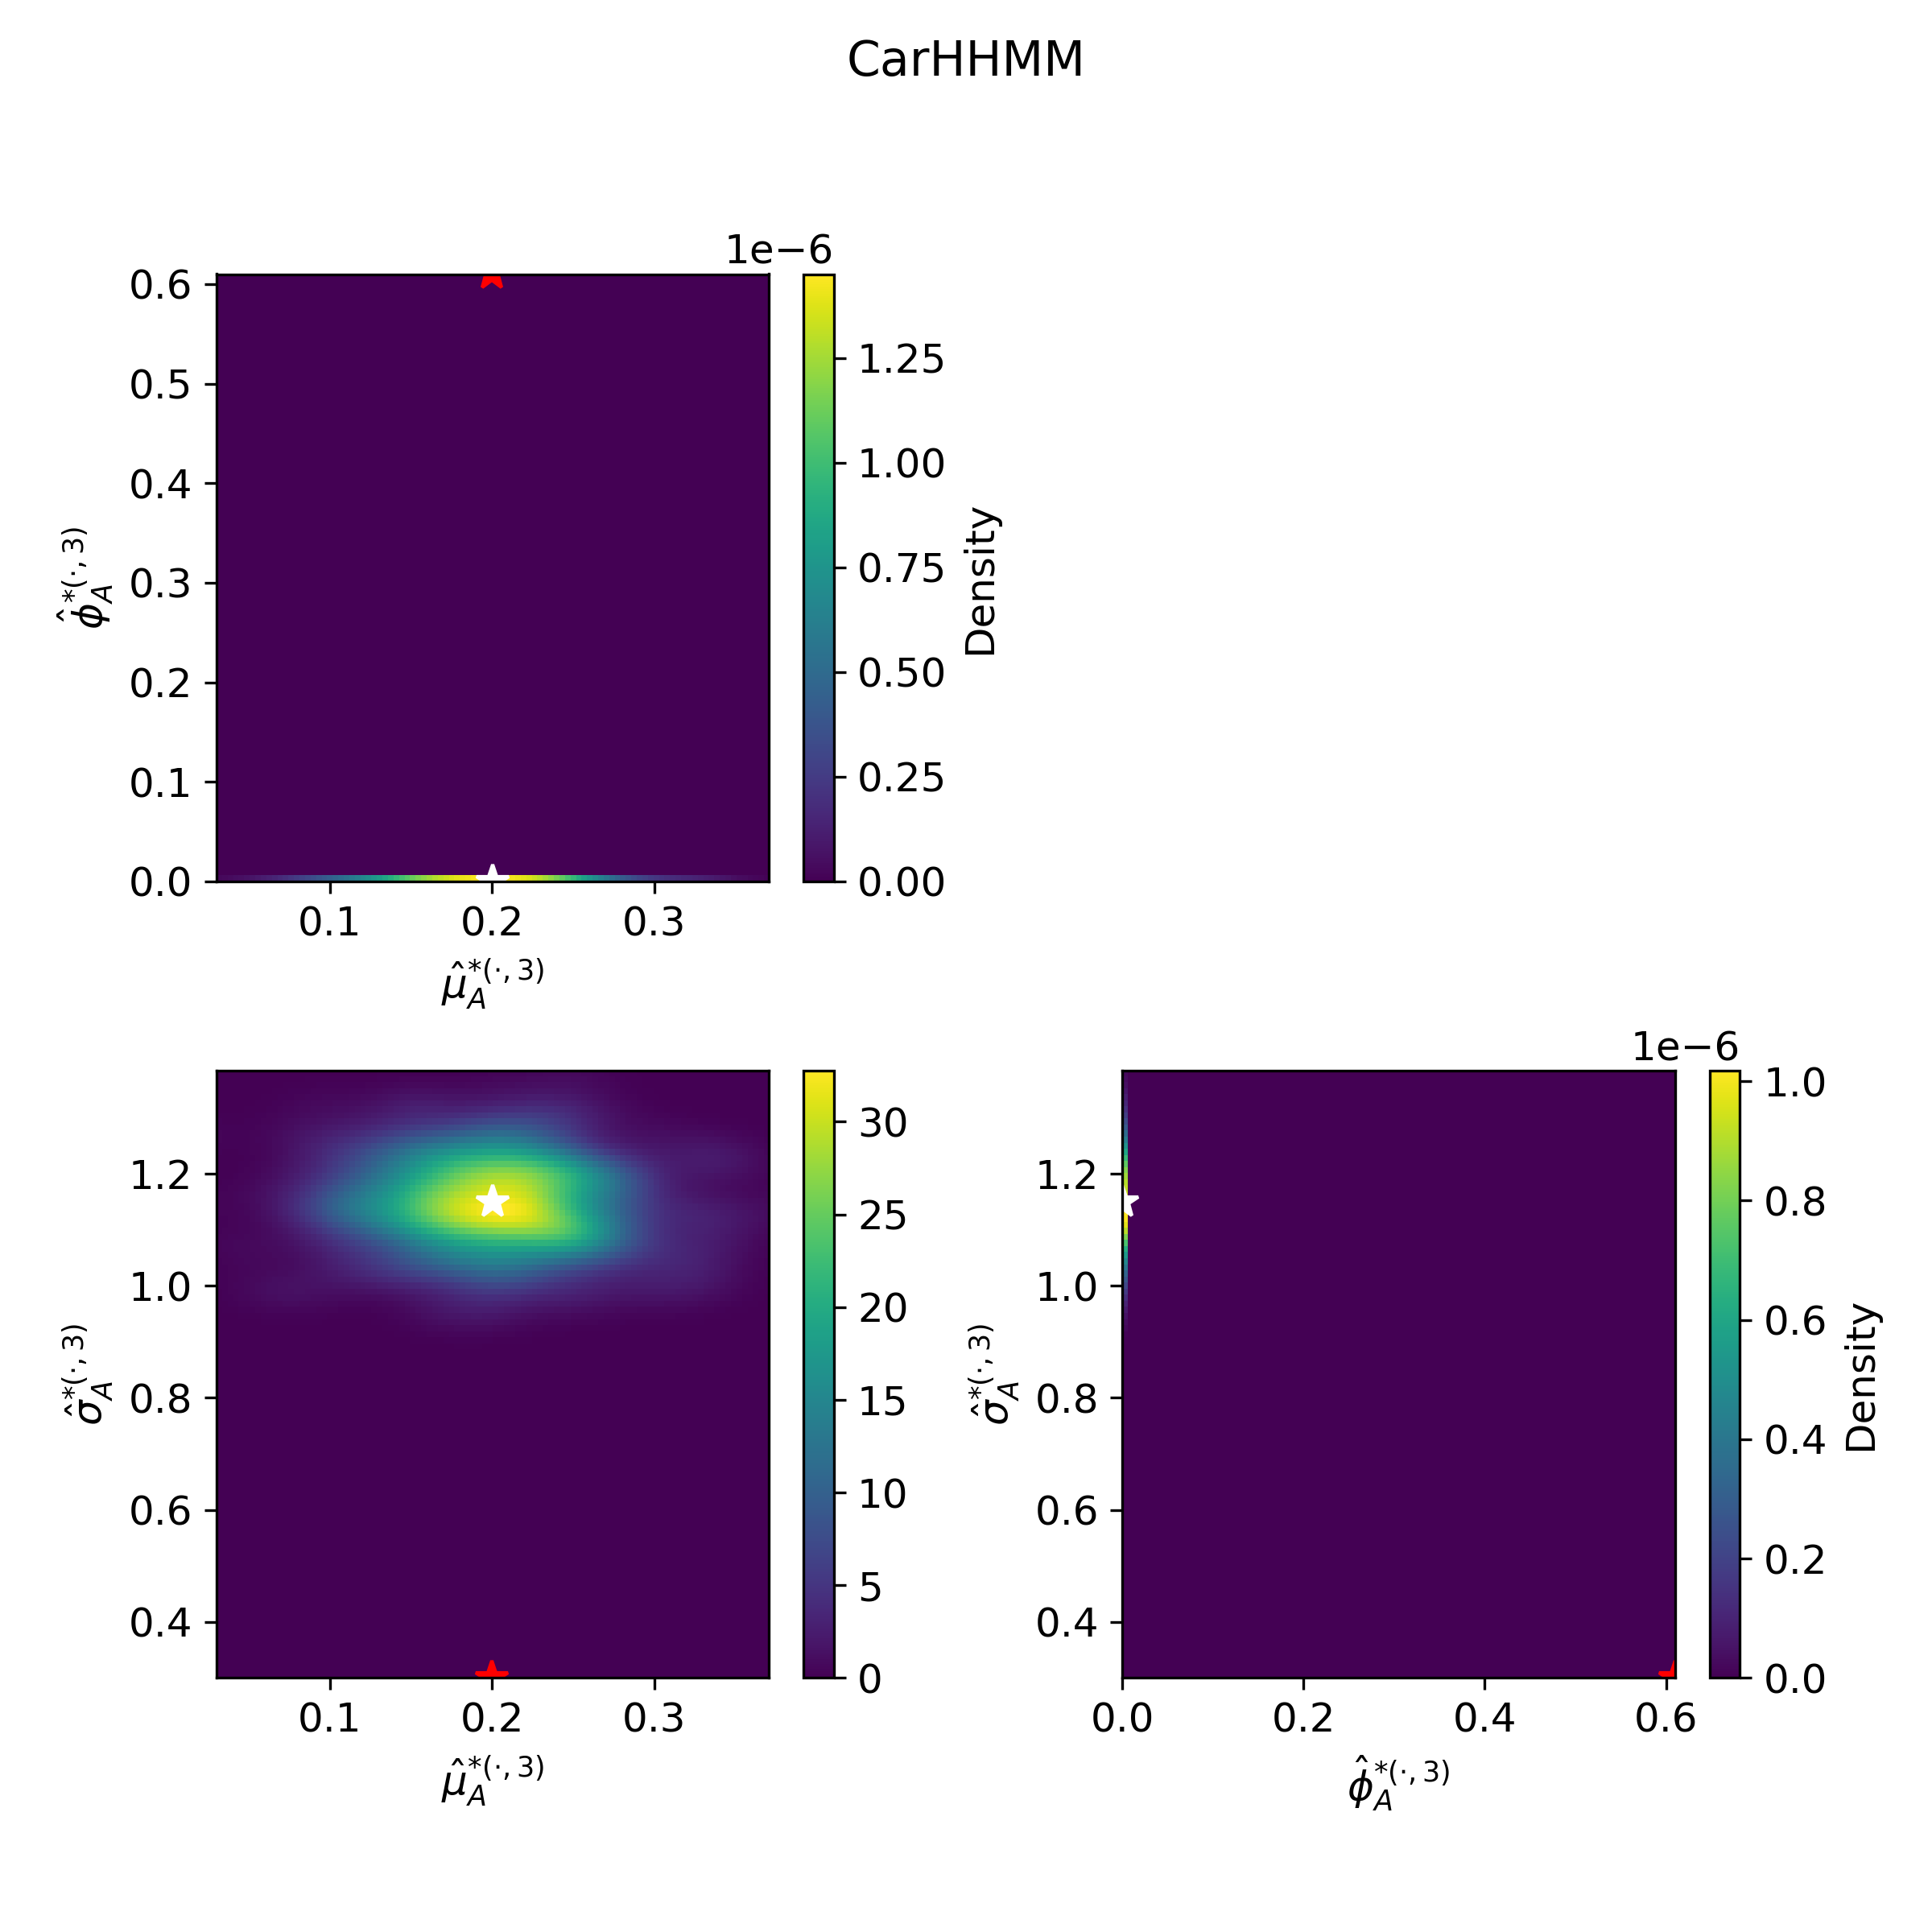
\includegraphics[width=2.1in]{../Plots/hhmm_V_MLE_density_A_0_2.png}
        \end{center}
        
        \noindent Figure \arabic{fignum}: Kernel density estimate of the distributions of estimates of acceleration parameters ($\hat \mu^*_A$, $\hat \sigma^*_A$, and $\hat \phi^*_A$) for each subdive state. The red star represents the true values of $\mu^*_A$, $\sigma^*_A$, and $\phi^*_A$ for both subdive states. These estimates are for the CarHHMM. 
        \addtocounter{fignum}{1}
        
        \subsection{CarHMM-DFT}
        \begin{center}
        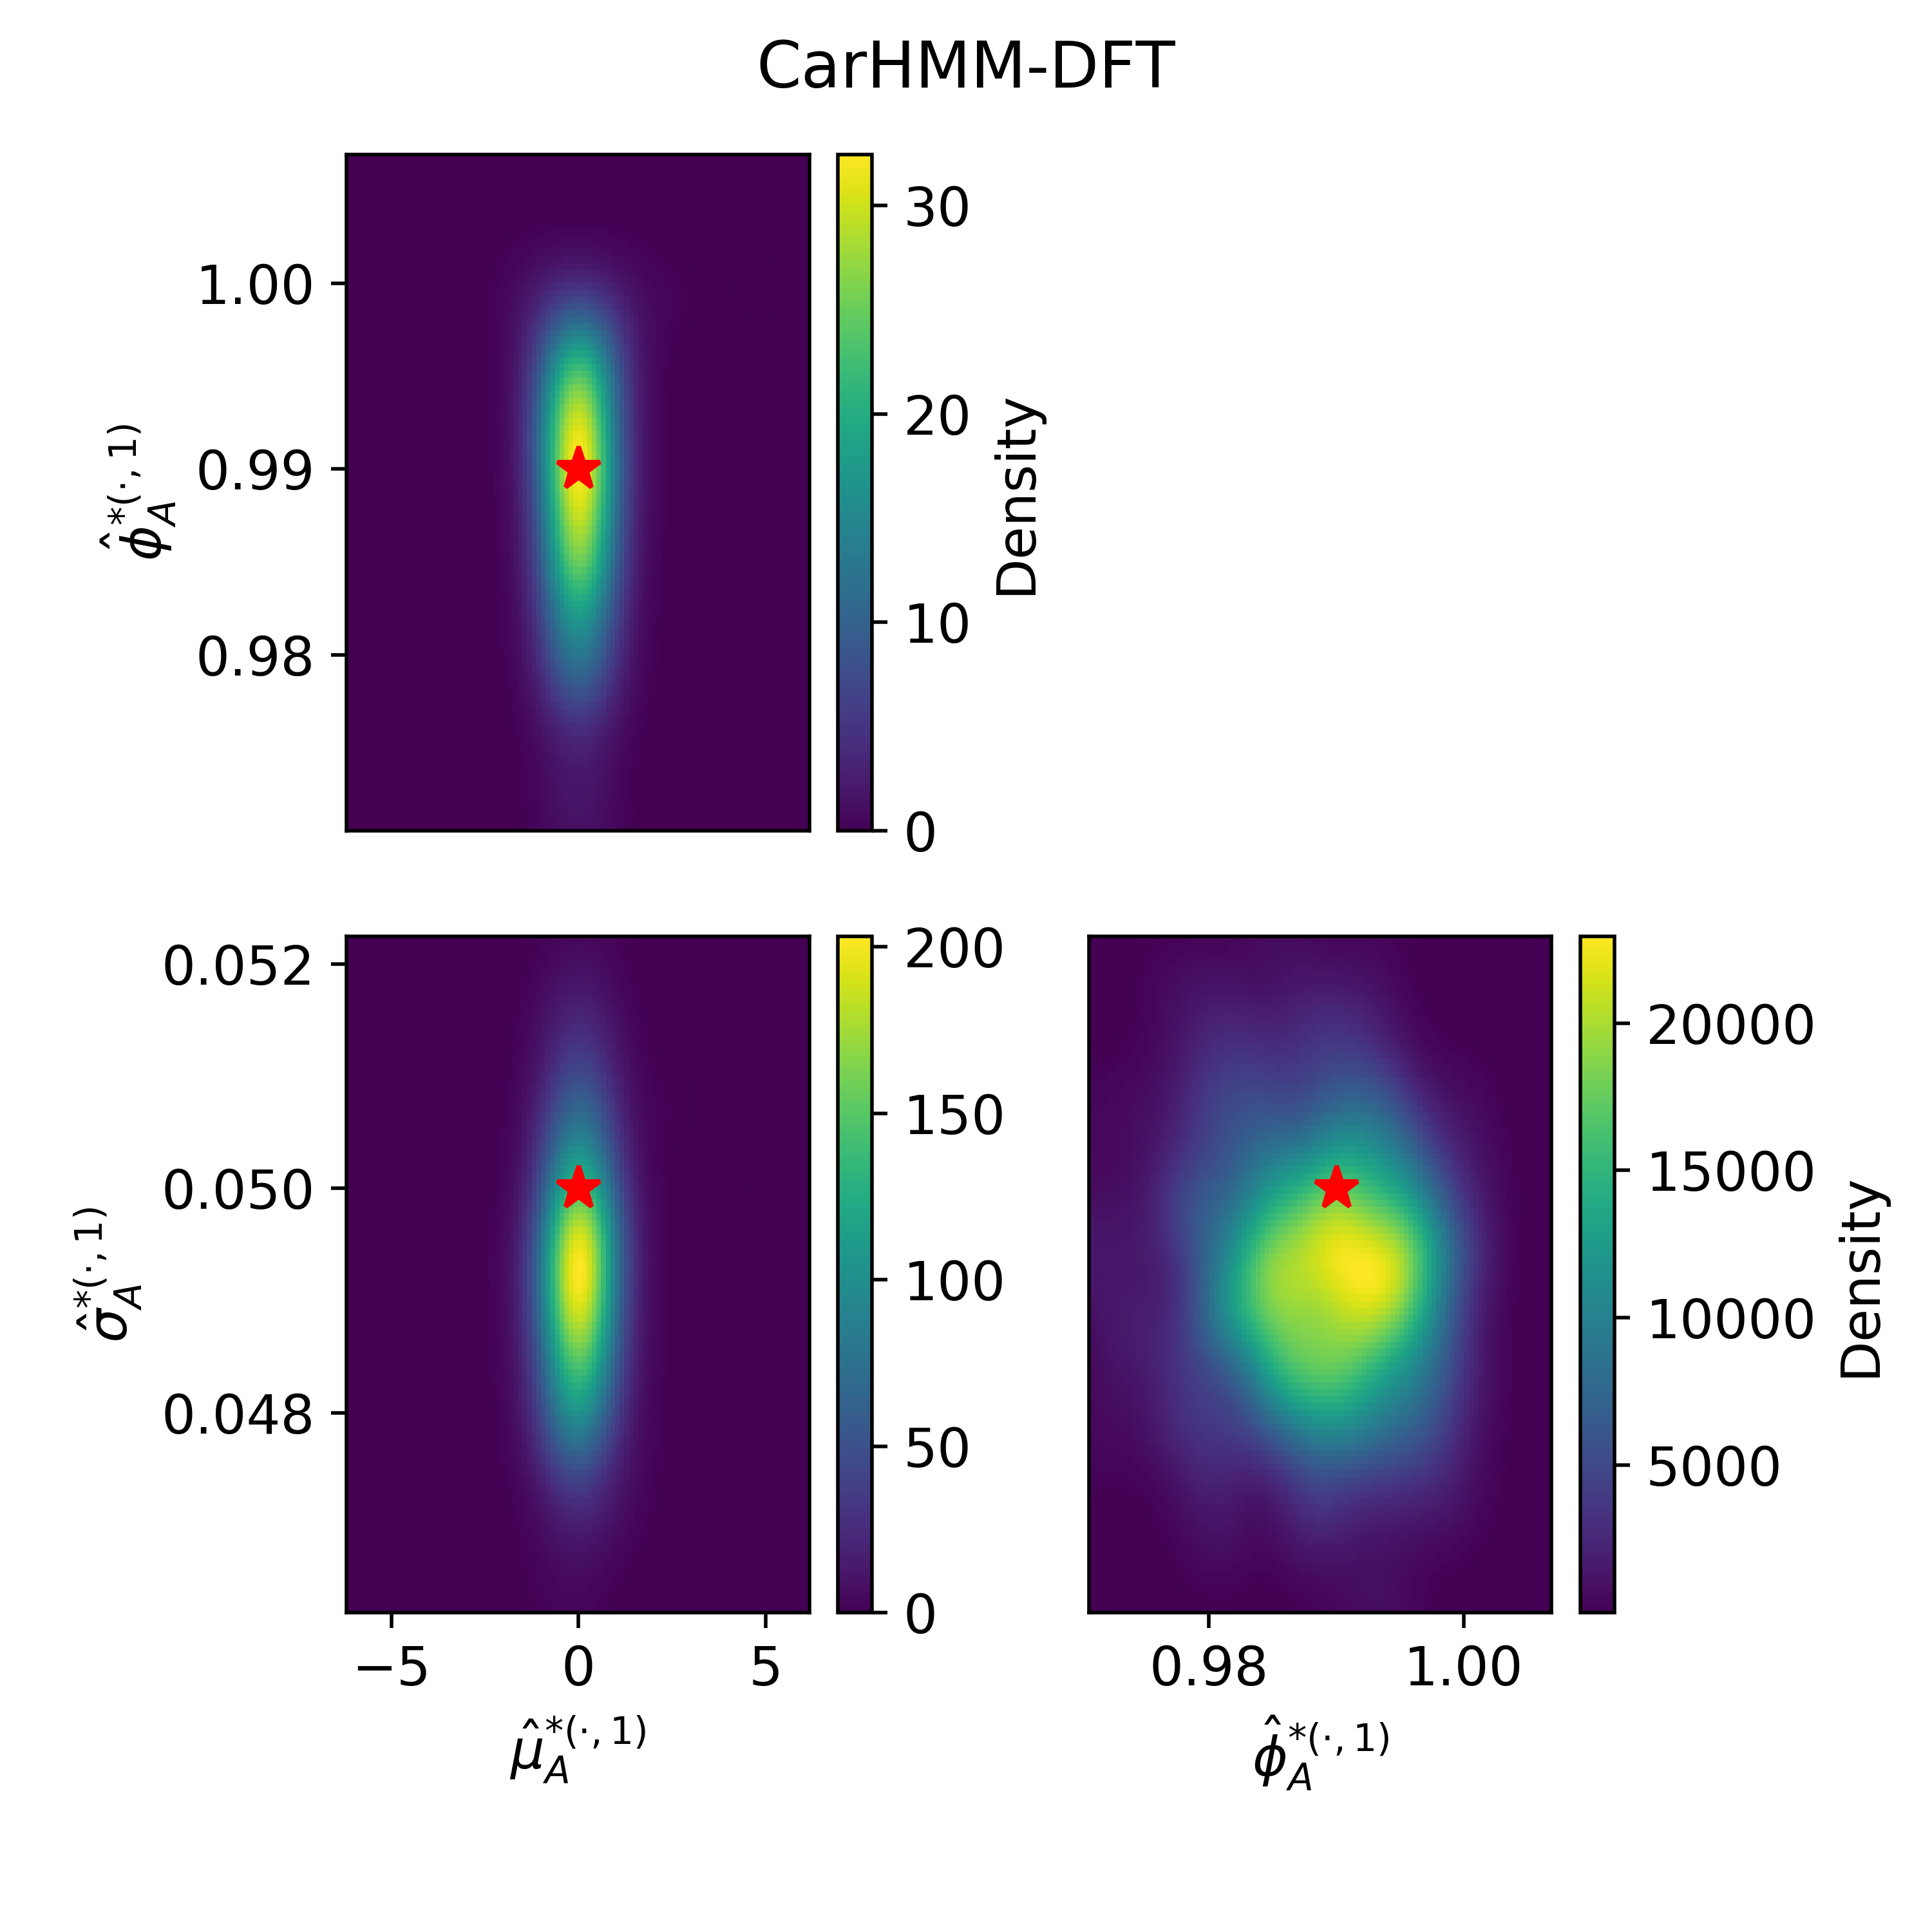
\includegraphics[width=2.1in]{../Plots/hmm_FV_MLE_density_A_0_0.png}
        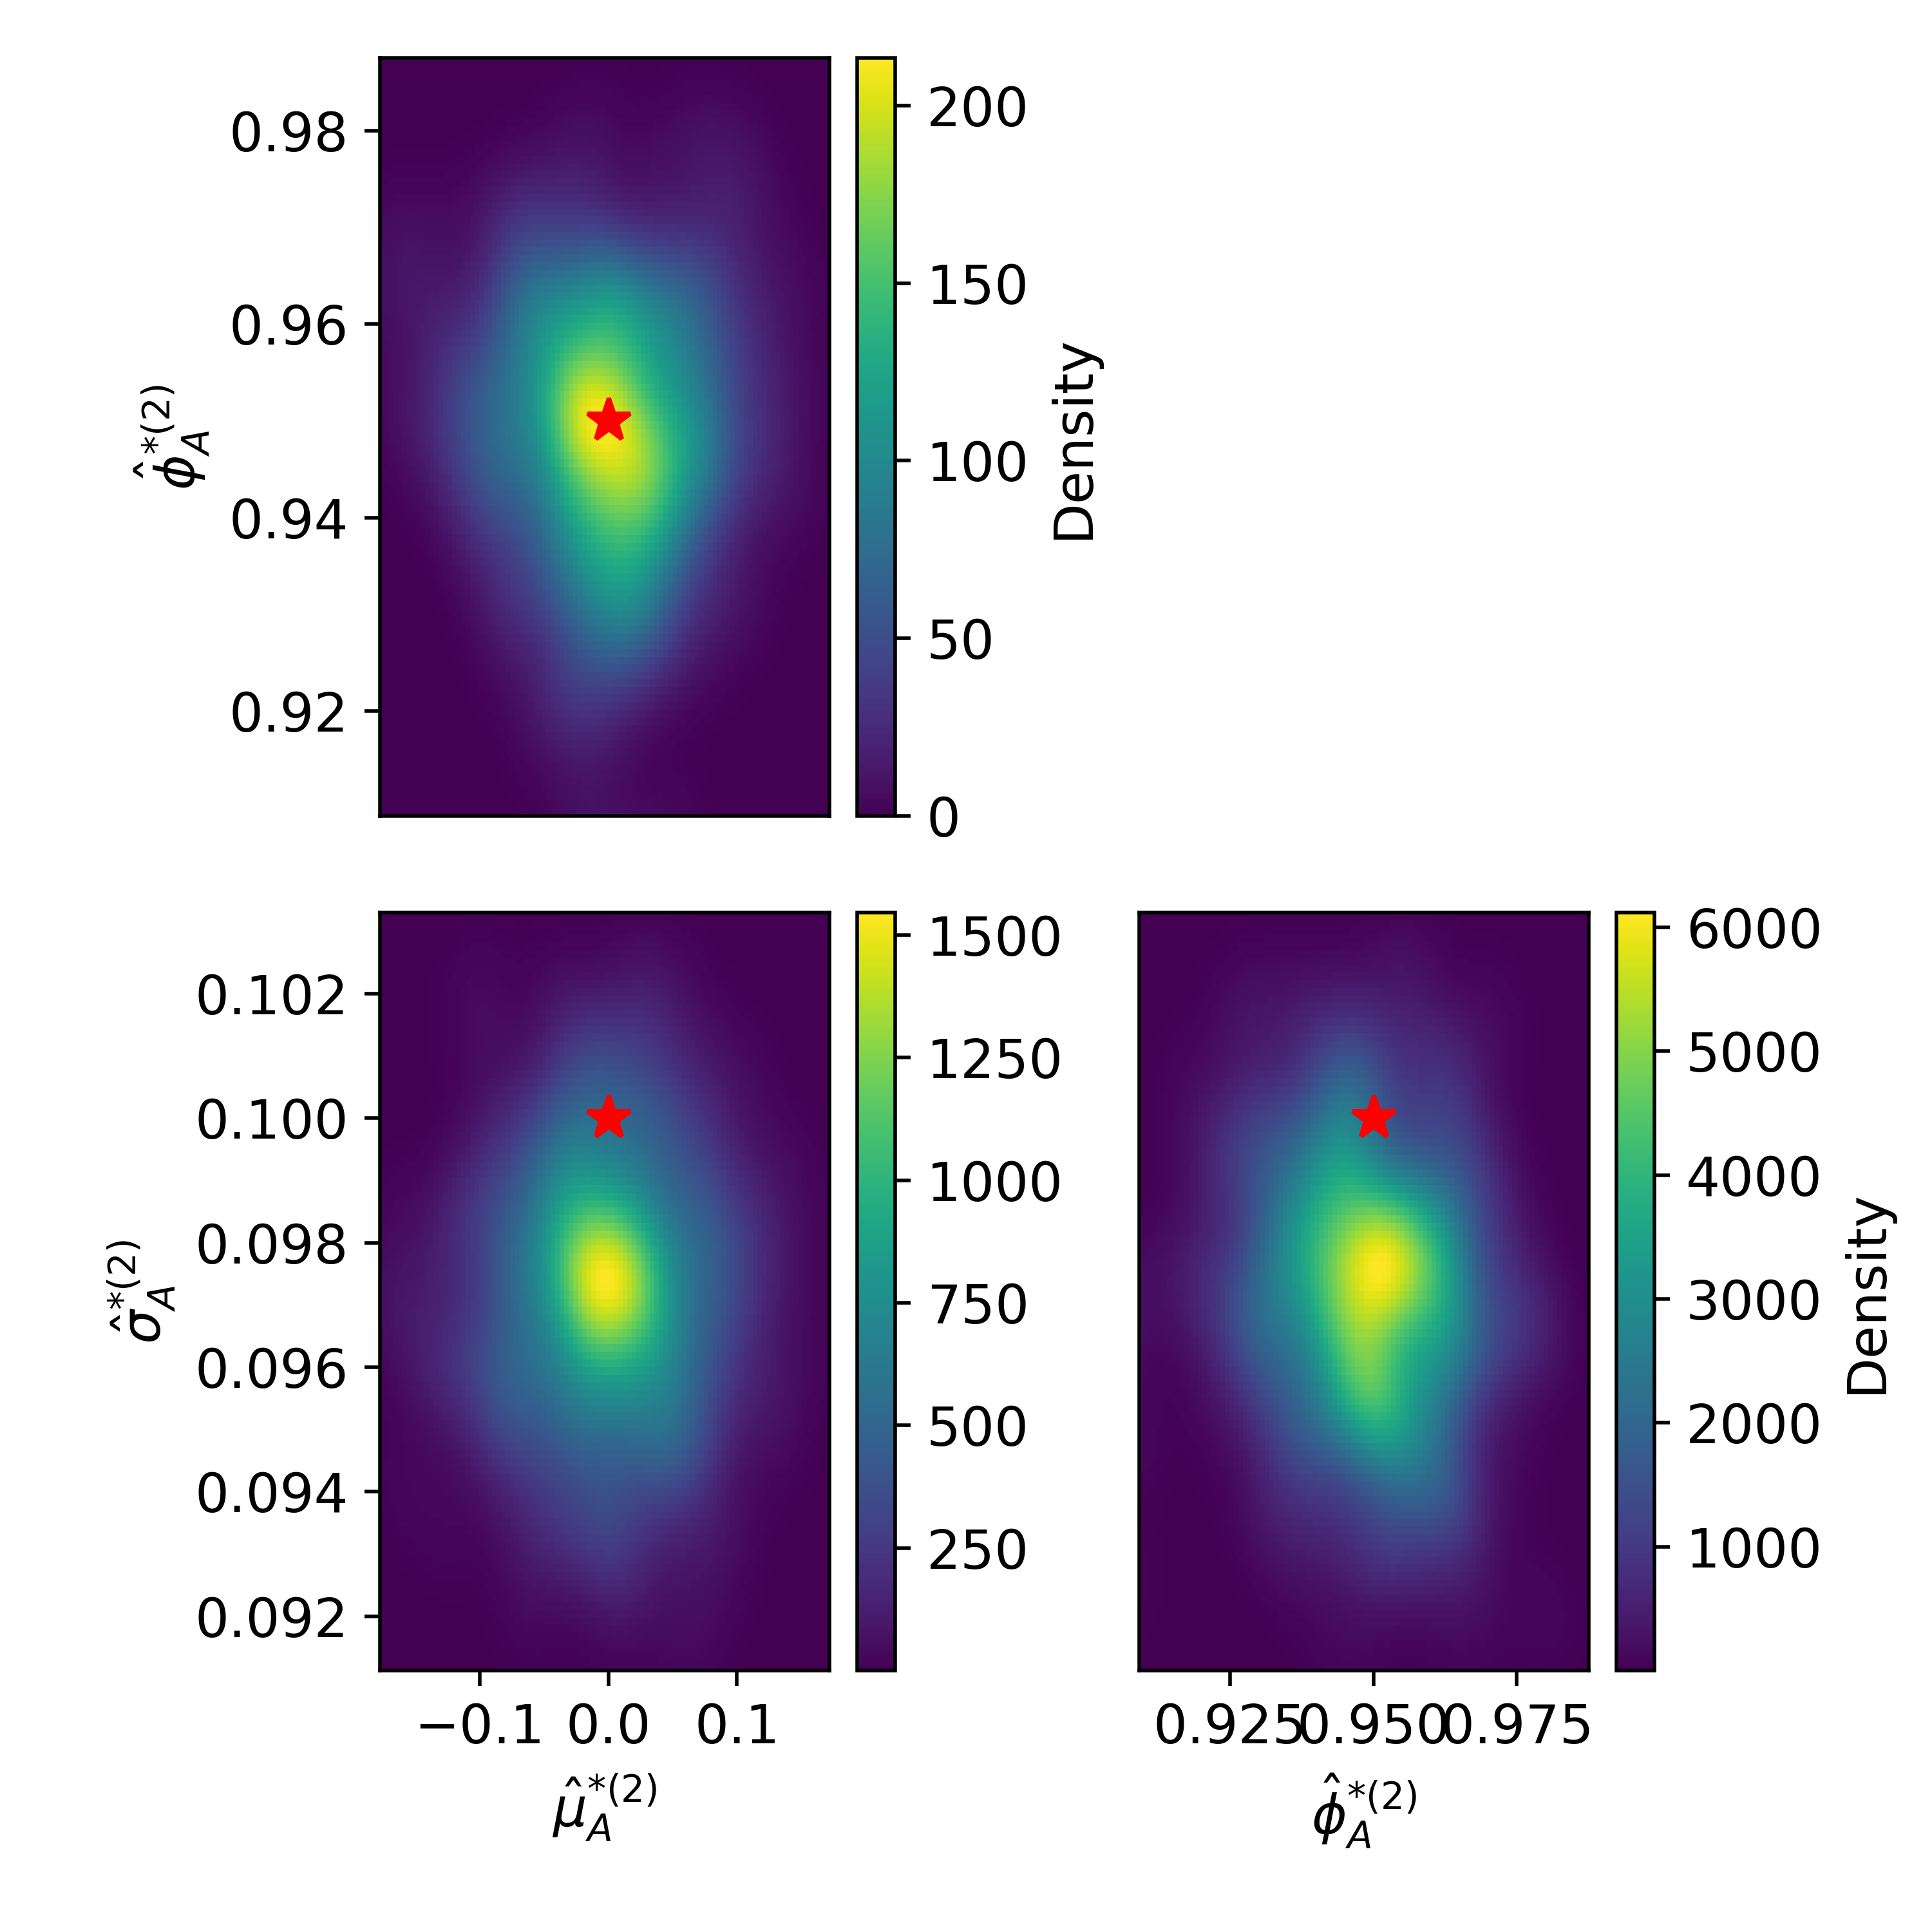
\includegraphics[width=2.1in]{../Plots/hmm_FV_MLE_density_A_0_1.png}
        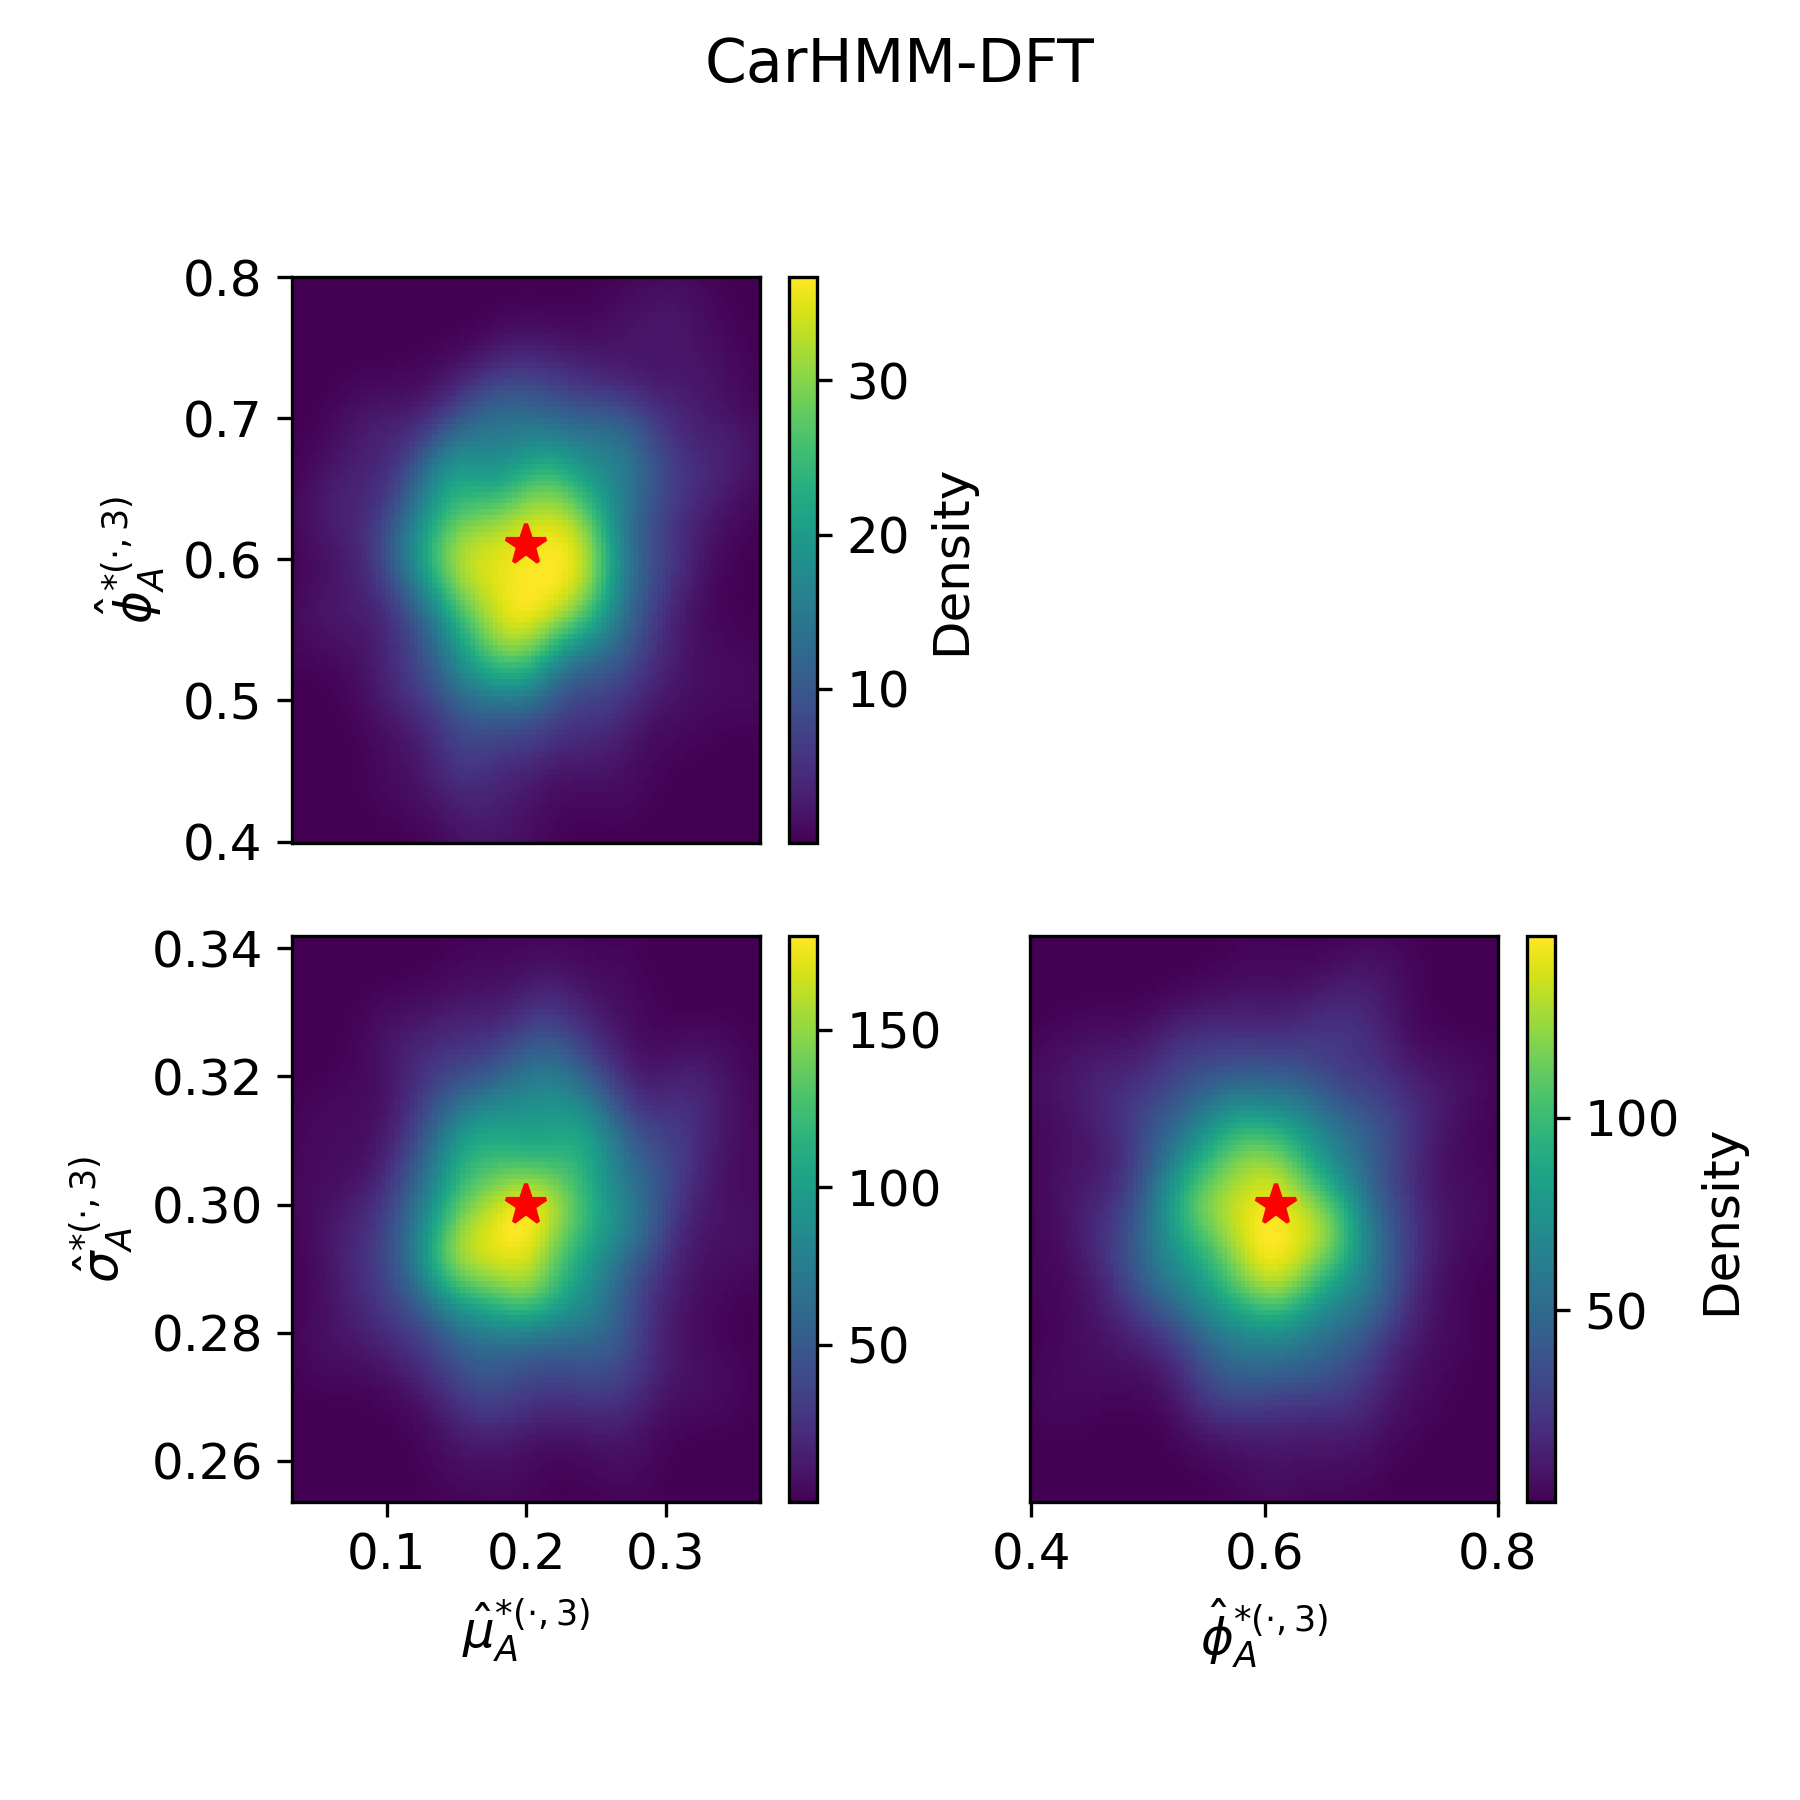
\includegraphics[width=2.1in]{../Plots/hmm_FV_MLE_density_A_0_2.png}
        \end{center}
        
        \noindent Figure \arabic{fignum}: Kernel density estimate of the distributions of estimates of acceleration parameters ($\hat \mu^*_A$, $\hat \sigma^*_A$, and $\hat \phi^*_A$) for each subdive state. The red star represents the true values of $\mu^*_A$, $\sigma^*_A$, and $\phi^*_A$ for both subdive states. These estimates are for the CarHMM-DFT.
        \addtocounter{fignum}{1}
        
    \newpage
    \section{Empirical joint distributions - wiggliness ($\Ztwo_{t,\tilde t^*}$)}
    
        \begin{center}
        \scalebox{0.75}{
        \bgroup
        \centering
        \def\arraystretch{1.5}
\begin{tabular}{ccccccc}
Model                       & \multicolumn{1}{c}{Parameter} & \multicolumn{1}{c}{Subdive Type} & \multicolumn{1}{c}{Estimate}   & \multicolumn{1}{c}{Bias}   & \multicolumn{1}{c}{Empirical SE} & \multicolumn{1}{c}{Observed Fischer SE}       \\ \hline
\multirow{6}{*}{CarHHMM-DFT}& \multirow{3}{*}{$\mu_W^*$}    & 1                                & $34.981$                         & $0.001$ $(p=0.978)$          & $1.026$                             & $0.658 \pm 0.088$                             \\
                            &                               & 2                                & $505.10$                         & $-0.69$ $(p=0.394)$          & $17.94$                             & $9.74 \pm 0.81$                             \\
                            &                               & 3                                & $9787.1$                         & $17.2$ $(p=0.718)$           & $1060.5$                            & $280.2 \pm 97.1$                             \\
                            & \multirow{3}{*}{$\sigma_W^*$} & 1                                & $23.849$                         & $-0.001$ $(p=0.991)$         & $0.989$                             & $0.652 \pm 0.094$                             \\
                            &                               & 2                                & $514.21$                         & $-2.47$ $(p=0.010)$          & $21.43$                             & $11.41 \pm 0.95$                             \\
                            &                               & 3                                & $14430$                          & $-33$ $(p=0.647)$            & $1596$                              & $303 \pm 166$                             \\ \hline
\multirow{6}{*}{HHMM-DFT}   & \multirow{3}{*}{$\mu_W^*$}    & 1                                & $35.067$                         & $0.087$ $(p=0.097)$          & $1.170$                             & $0.679 \pm 0.100$                             \\
                            &                               & 2                                & $500.93$                         & $-4.86$ $(p=0.000)$          & $24.02$                             & $10.75 \pm 1.21$                             \\
                            &                               & 3                                & $6841.0$                         & $-2929.0$ $(p=0.000)$        & $1164.3$                            & $198.2 \pm 74.7$                             \\
                            & \multirow{3}{*}{$\sigma_W^*$} & 1                                & $23.800$                         & $-0.050$ $(p=0.351)$         & $1.192$                             & $0.676 \pm 0.104$                             \\
                            &                               & 2                                & $513.26$                         & $-3.42$ $(p=0.001)$          & $22.60$                             & $12.50 \pm 1.30$                             \\
                            &                               & 3                                & $11459$                          & $-3004$ $(p=0.000)$          & $1739$                              & $303 \pm 194$                             \\ \hline
\multirow{6}{*}{CarHHMM}    & \multirow{3}{*}{$\mu_W^*$}    & 1                                & ------                         & ------                     & ------                             & ------                                      \\
                            &                               & 2                                & ------                         & ------                     & ------                             & ------                                      \\
                            &                               & 3                                & ------                         & ------                     & ------                             & ------                                      \\
                            & \multirow{3}{*}{$\sigma_W^*$} & 1                                & ------                         & ------                     & ------                             & ------                                      \\
                            &                               & 2                                & ------                         & ------                     & ------                             & ------                                      \\
                            &                               & 3                                & ------                         & ------                     & ------                             & ------                                      \\ \hline
\multirow{6}{*}{CarHMM-DFT} & \multirow{3}{*}{$\mu_W^*$}    & 1                                & $35.034$                         & $0.054$ $(p=0.264)$          & $1.076$                             & $0.661 \pm 0.093$                             \\ 
                            &                               & 2                                & $503.76$                         & $-2.03$ $(p=0.013)$          & $18.26$                             & $9.64 \pm 0.92$                             \\
                            &                               & 3                                & $9817.8$                         & $47.8$ $(p=0.328)$          & $1089.1$                             & $280.2 \pm 136.3$                             \\
                            & \multirow{3}{*}{$\sigma_W^*$} & 1                                & $23.890$                         & $0.040$ $(p=0.401)$          & $1.058$                             & $0.656 \pm 0.101$                             \\
                            &                               & 2                                & $515.23$                         & $-1.45$ $(p=0.125)$          & $21.09$                             & $11.37 \pm 0.99$                             \\
                            &                               & 3                                & $14437$                          & $-25$ $(p=0.740)$          & $1661$                             & $332 \pm 166$                             \\
\end{tabular}
        \egroup
        }
        \end{center}
        
        \noindent Table \arabic{tablenum}: Estimates and standard errors for the parameters of the distribution of wiggliness across all four models in the simulation study. The ``Estimate" column is the average across 500 simulations, and the ``Observed Fisher SE" column is the median across 500 simulations. The $\pm$ refers to the inter-quartile range. SE stands for standard error. Reported $p$-values test if the observed bias is statistically significant using a one-sample $t$-test.
        \addtocounter{tablenum}{1}
        
        \newpage
    
        \subsection{CarHHMM-DFT}
        \begin{center}
        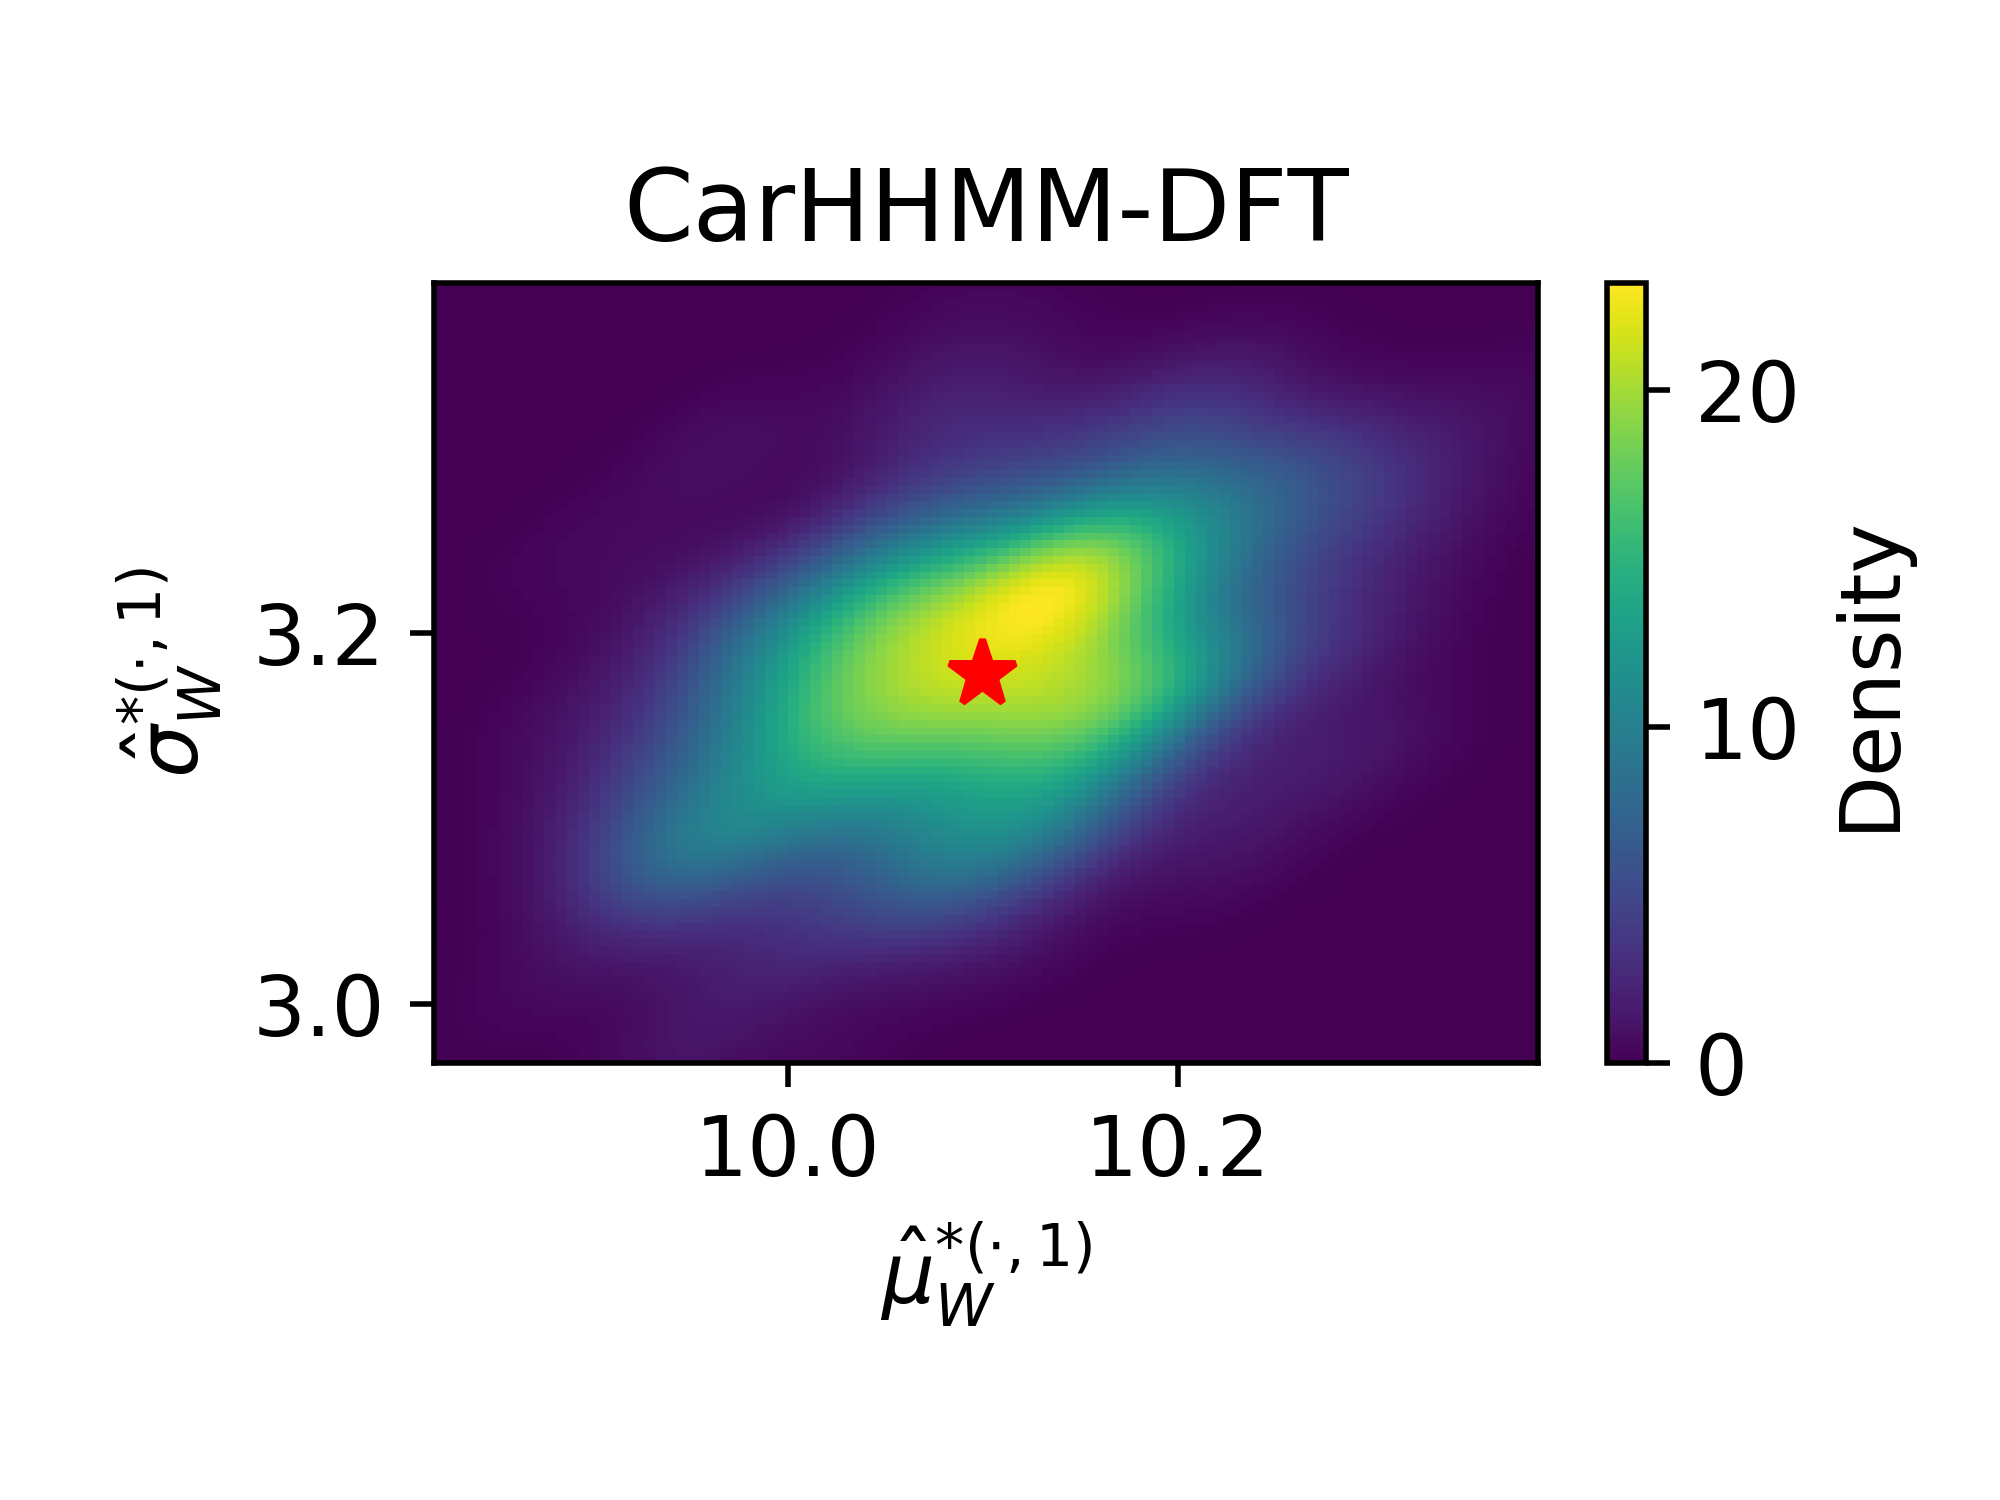
\includegraphics[width=2.1in]{../Plots/hhmm_FV_MLE_density_FoVeDBA_0_0.png}
        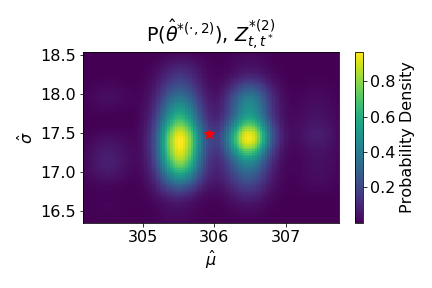
\includegraphics[width=2.1in]{../Plots/hhmm_FV_MLE_density_FoVeDBA_0_1.png}
        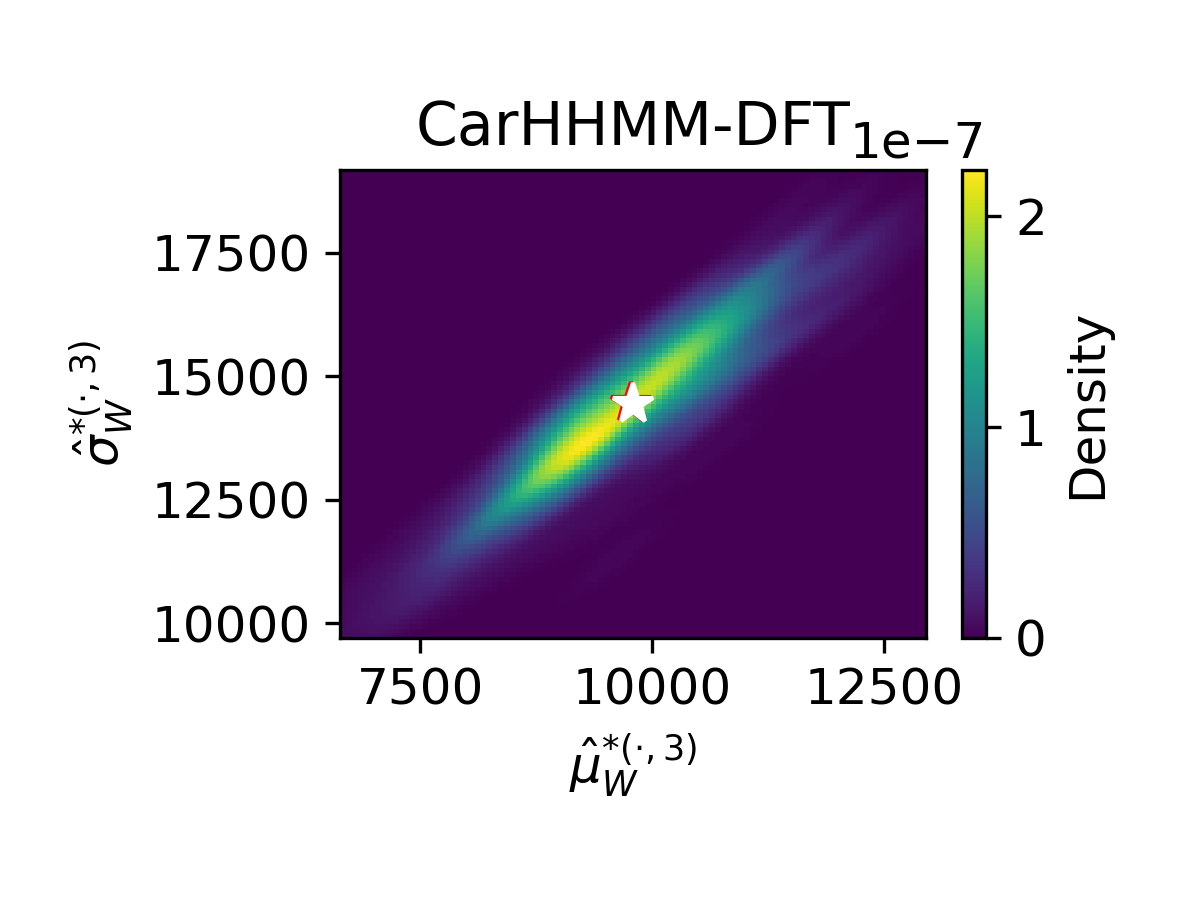
\includegraphics[width=2.1in]{../Plots/hhmm_FV_MLE_density_FoVeDBA_0_2.png}
        \end{center}
        
        \noindent Figure \arabic{fignum}: Kernel density estimate of the distributions of estimates of wiggliness parameters ($\hat \mu^*_W$ and $\hat \sigma^*_W$) for each subdive state. The red star represents the true values of $\mu^*_W$ and $\sigma^*_W$ for both subdive states. These estimates are for the CarHHMM-DFT.
        \addtocounter{fignum}{1}
        
        \subsection{HHMM-DFT}
        \begin{center}
        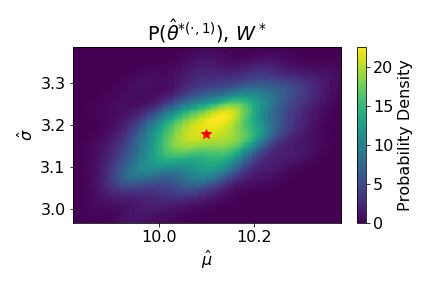
\includegraphics[width=2.1in]{../Plots/hhmm_FV_uncorr_MLE_density_FoVeDBA_0_0.png}
        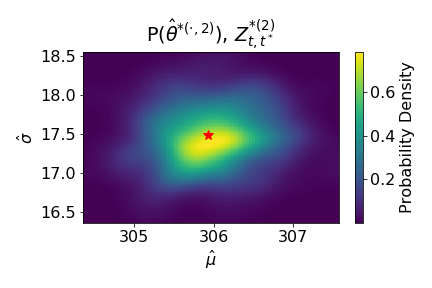
\includegraphics[width=2.1in]{../Plots/hhmm_FV_uncorr_MLE_density_FoVeDBA_0_1.png}
        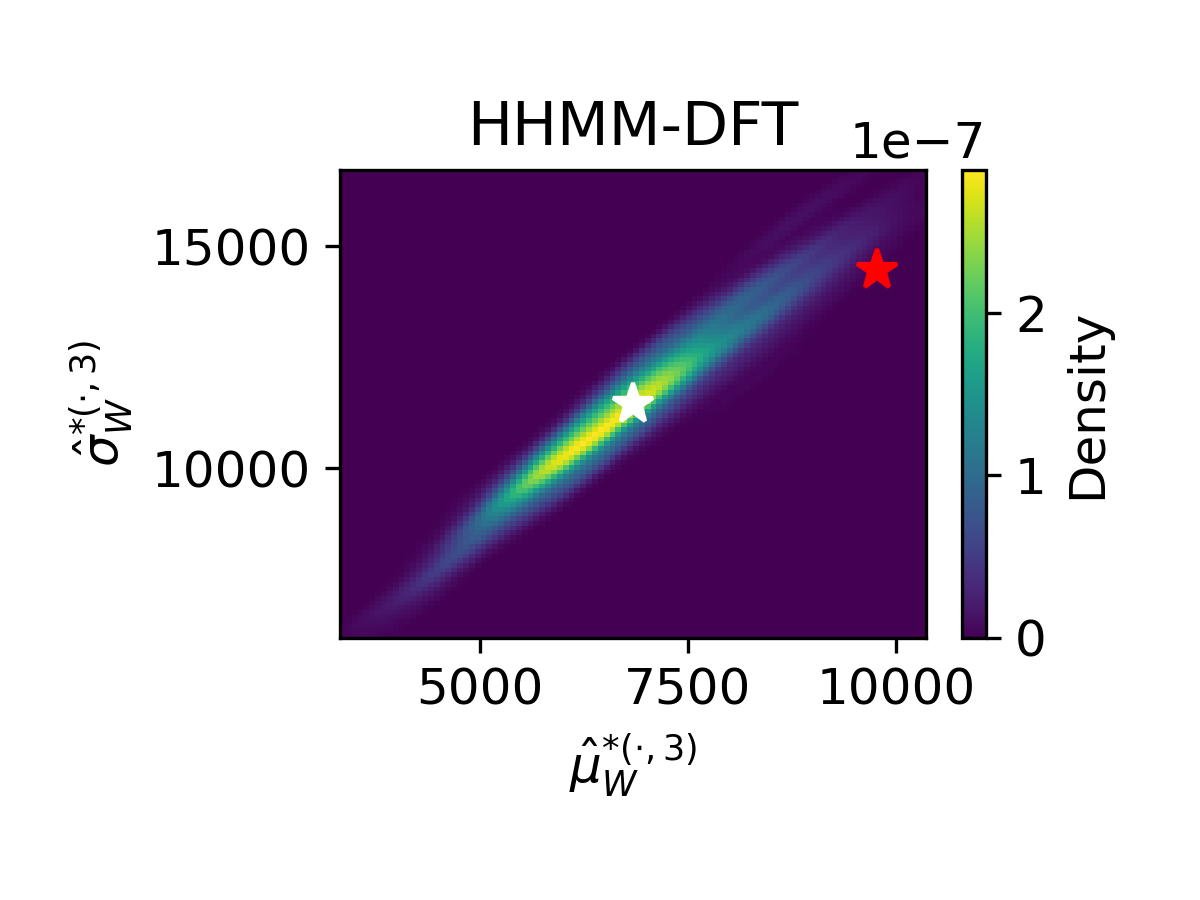
\includegraphics[width=2.1in]{../Plots/hhmm_FV_uncorr_MLE_density_FoVeDBA_0_2.png}
        \end{center}
        
        \noindent Figure \arabic{fignum}: Kernel density estimate of the distributions of estimates of wiggliness parameters ($\hat \mu^*_W$ and $\hat \sigma^*_W$) for each subdive state. The red star represents the true values of $\mu^*_W$ and $\sigma^*_W$ for both subdive states. These estimates are for the HHMM-DFT.
        \addtocounter{fignum}{1}
        
        \subsection{CarHHMM}
        The CarHHMM did not use wiggliness to model the whale's behaviour.
        
        \subsection{CarHMM-DFT}
        \begin{center}
        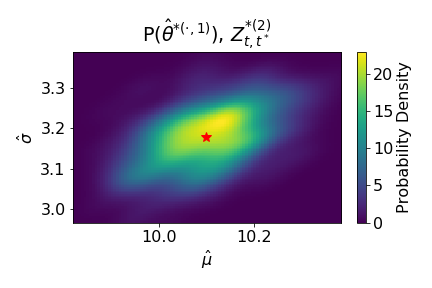
\includegraphics[width=2.1in]{../Plots/hmm_FV_MLE_density_FoVeDBA_0_0.png}
        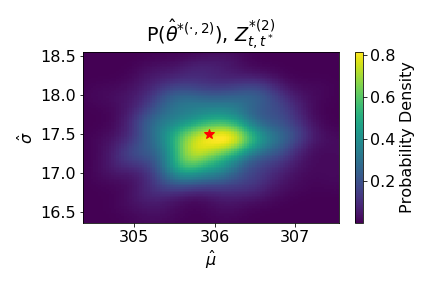
\includegraphics[width=2.1in]{../Plots/hmm_FV_MLE_density_FoVeDBA_0_1.png}
        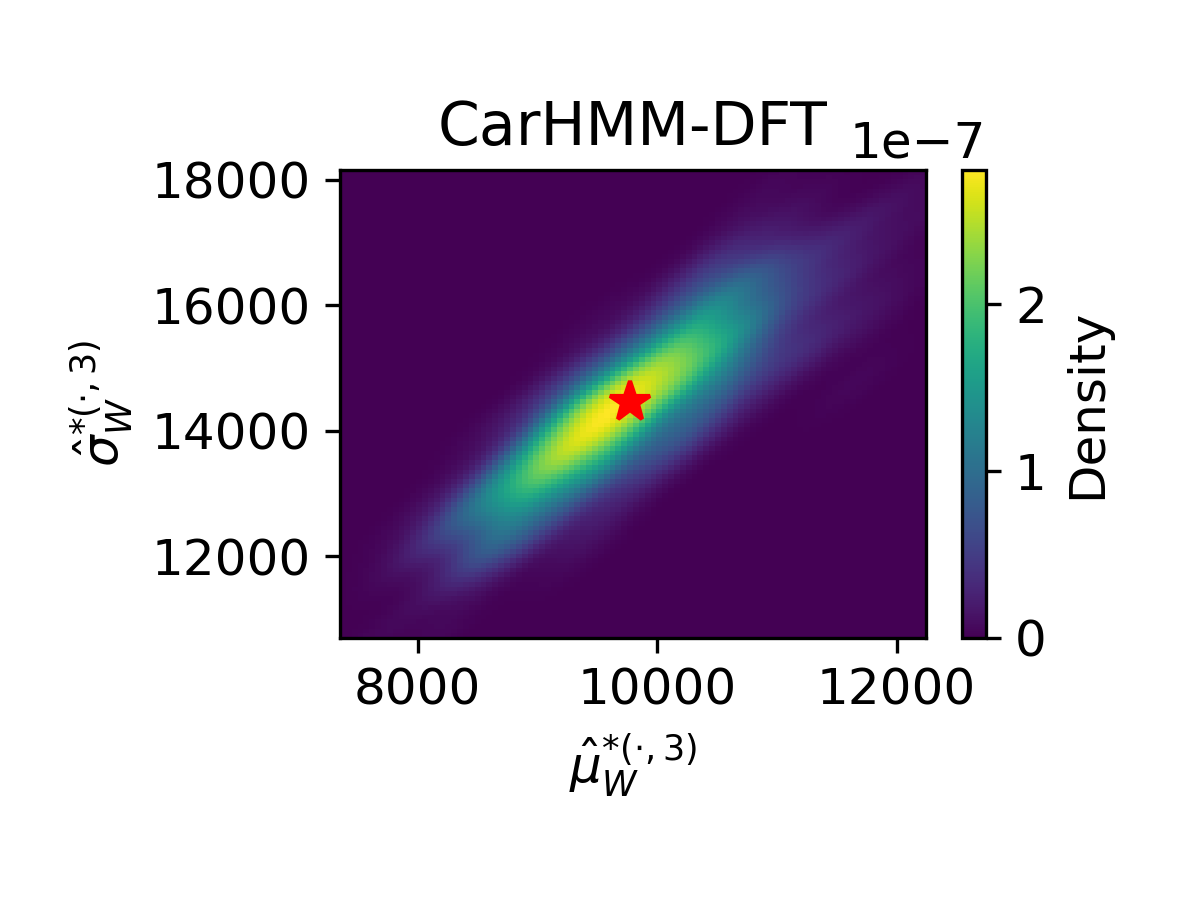
\includegraphics[width=2.1in]{../Plots/hmm_FV_MLE_density_FoVeDBA_0_2.png}
        \end{center}
        
        \noindent Figure \arabic{fignum}: Kernel density estimate of the distributions of estimates of wiggliness parameters ($\hat \mu^*_W$ and $\hat \sigma^*_W$) for each subdive state. The red star represents the true values of $\mu^*_W$ and $\sigma^*_W$ for both subdive states. These estimates are for the CarHMM-DFT.
        \addtocounter{fignum}{1}
        
    \newpage
    \section{Empirical joint distributions - probability transition matrices ($\Gamma, \Gamma^*$)}
        
        \begin{center}
        \scalebox{0.75}{
        \bgroup
        \centering
        \def\arraystretch{1.5}
\begin{tabular}{ccccccc}
Model                        & \multicolumn{1}{c}{Parameter} & \multicolumn{1}{c}{Estimate}   & \multicolumn{1}{c}{Bias} & \multicolumn{1}{c}{Empirical SE} & \multicolumn{1}{c}{Observed Fischer SE}     \\ \hline
\multirow{2}{*}{CarHHMM-DFT}& $\Gamma_{12}$                 & $0.160$                         & $0.005$ $(p=0.030)$        & $0.056$                           & $0.042 \pm 0.012$                             \\
                             & $\Gamma_{21}$                 & $0.907$                         & $-0.006$ $(p=0.214)$        & $0.102$                           & $0.116$                             \\ \hline
\multirow{2}{*}{HHMM-DFT}   & $\Gamma_{12}$                 & $0.161$                         & $0.007$ $(p=0.007)$        & $0.055$                           & $0.041 \pm 0.011$                             \\
                             & $\Gamma_{21}$                 & $0.916$                         & $0.004$ $(p=0.372)$        & $0.088$                           & $0.112$                             \\ \hline
\multirow{2}{*}{CarHHMM}    & $\Gamma_{12}$                 & $0.198$                         & $0.044$ $(p=0.000)$        & $0.152$                           & $0.044 \pm 0.014$                             \\
                             & $\Gamma_{21}$                 & $0.832$                         & $-0.081$ $(p=0.000)$        & $0.195$                           & $0.103 \pm 0.073$                             \\ \hline
\multirow{2}{*}{CarHMM-DFT} & $\Gamma_{12}$                 & ------                         & ------                   & ------                           & ------                                      \\
                             & $\Gamma_{21}$                 & ------                         & ------                   & ------                           & ------                                      \\
\end{tabular}
        \egroup
        }
        \end{center}
        
        \noindent Table \arabic{tablenum}: Estimates and standard errors for coarse-scale probability transition matrices across all four models in the simulation study. The ``Estimate" column is the average across 500 simulations, and the ``Observed Fisher SE" column is the median across 500 simulations. The $\pm$ refers to the inter-quartile range. SE stands for standard error. Reported $p$-values test if the observed bias is statistically significant using a one-sample $t$-test.
        \addtocounter{tablenum}{1}
        
        \newpage
        
        \begin{center}
        \scalebox{0.7}{
        \bgroup
        \centering
        \def\arraystretch{1.5}
\begin{tabular}{ccccccc}
Model                        & \multicolumn{1}{c}{Parameter} & \multicolumn{1}{c}{Estimate}   & \multicolumn{1}{c}{Bias} & \multicolumn{1}{c}{Empirical SE} & \multicolumn{1}{c}{Observed Fischer SE}     \\ \hline
\multirow{12}{*}{CarHHMM-DFT}& $\Gamma^{*(1)}_{12}$          & $0.258$                         & $0.006$ $(p=0.004)$        & $0.043$                           & $0.032 \pm 0.006$                             \\
                             & $\Gamma^{*(1)}_{13}$          & $0.002$                         & $0.002$ $(p=0.000)$        & $0.004$                           & $\text{N/A}$                             \\
                             & $\Gamma^{*(1)}_{21}$          & $0.083$                         & $0.001$ $(p=0.243)$        & $0.015$                           & $0.012 \pm 0.002$                             \\
                             & $\Gamma^{*(1)}_{23}$          & $0.052$                         & $-0.000$ $(p=0.984)$        & $0.010$                           & $0.009 \pm 0.001$                             \\
                             & $\Gamma^{*(1)}_{31}$          & $0.003$                         & $0.003$ $(p=0.000)$        & $0.008$                           & $\text{N/A}$                             \\
                             & $\Gamma^{*(1)}_{32}$          & $0.234$                         & $0.002$ $(p=0.322)$        & $0.042$                           & $0.036 \pm 0.008$                             \\
                             & $\Gamma^{*(2)}_{12}$          & $0.111$                         & $0.146$ $(p=0.349)$        & $0.017$                           & $0.015 \pm 0.004$                             \\
                             & $\Gamma^{*(2)}_{13}$          & $0.001$                         & $0.002$ $(p=0.000)$        & $0.002$                           & $\text{N/A}$                             \\
                             & $\Gamma^{*(2)}_{21}$          & $0.151$                         & $-0.068$ $(p=0.584)$        & $0.023$                           & $0.021 \pm 0.005$                             \\
                             & $\Gamma^{*(2)}_{23}$          & $0.036$                         & $0.016$ $(p=0.944)$        & $0.013$                           & $0.010 \pm 0.003$                             \\
                             & $\Gamma^{*(2)}_{31}$          & $0.007$                         & $0.003$ $(p=0.000)$        & $0.024$                           & $\text{N/A}$                             \\
                             & $\Gamma^{*(2)}_{32}$          & $0.252$                         & $0.008$ $(p=0.000)$        & $0.096$                           & $0.063 \pm 0.028$                             \\ \hline
\multirow{12}{*}{HHMM-DFT}   & $\Gamma^{*(1)}_{12}$          & $0.240$                         & $-0.012$ $(p=0.000)$        & $0.042$                           & $0.032 \pm 0.006$                             \\
                             & $\Gamma^{*(1)}_{13}$          & $0.003$                         & $0.003$ $(p=0.000)$        & $0.006$                           & $\text{N/A}$                             \\
                             & $\Gamma^{*(1)}_{21}$          & $0.077$                         & $-0.005$ $(p=0.000)$        & $0.019$                           & $0.012 \pm 0.002$                             \\
                             & $\Gamma^{*(1)}_{23}$          & $0.047$                         & $-0.004$ $(p=0.000)$        & $0.009$                           & $0.008 \pm 0.001$                             \\
                             & $\Gamma^{*(1)}_{31}$          & $0.005$                         & $0.005$ $(p=0.000)$        & $0.009$                           & $\text{N/A}$                             \\
                             & $\Gamma^{*(1)}_{32}$          & $0.153$                         & $-0.079$ $(p=0.000)$        & $0.029$                           & $0.026 \pm 0.005$                             \\
                             & $\Gamma^{*(2)}_{12}$          & $0.109$                         & $0.128$ $(p=0.000)$        & $0.018$                           & $0.016 \pm 0.004$                             \\
                             & $\Gamma^{*(2)}_{13}$          & $0.002$                         & $0.003$ $(p=0.000)$        & $0.004$                           & $\text{N/A}$                             \\
                             & $\Gamma^{*(2)}_{21}$          & $0.151$                         & $-0.073$ $(p=0.712)$        & $0.031$                           & $0.023 \pm 0.006$                             \\
                             & $\Gamma^{*(2)}_{23}$          & $0.037$                         & $0.012$ $(p=0.009)$        & $0.013$                           & $0.011 \pm 0.004$                             \\
                             & $\Gamma^{*(2)}_{31}$          & $0.021$                         & $0.005$ $(p=0.000)$        & $0.026$                           & $0.034  $                             \\
                             & $\Gamma^{*(2)}_{32}$          & $0.135$                         & $-0.073$ $(p=0.000)$        & $0.057$                           & $0.038 \pm 0.018$                             \\ \hline
\multirow{12}{*}{CarHHMM}    & $\Gamma^{*(1)}_{12}$          & $0.138$                         & $-0.114$ $(p=0.000)$        & $0.131$                           & $0.018 \pm 0.006$                             \\
                             & $\Gamma^{*(1)}_{13}$          & $0.023$                         & $0.022$ $(p=0.000)$        & $0.107$                           & $0.039  $                             \\
                             & $\Gamma^{*(1)}_{21}$          & $0.037$                         & $-0.044$ $(p=0.000)$        & $0.054$                           & $0.007 \pm 0.001$                             \\
                             & $\Gamma^{*(1)}_{23}$          & $0.027$                         & $-0.025$ $(p=0.000)$        & $0.050$                           & $0.004 \pm 0.001$                             \\
                             & $\Gamma^{*(1)}_{31}$          & $0.013$                         & $0.013$ $(p=0.000)$        & $0.022$                           & $0.013  $                             \\
                             & $\Gamma^{*(1)}_{32}$          & $0.134$                         & $-0.099$ $(p=0.000)$        & $0.043$                           & $0.023 \pm 0.006$                             \\
                             & $\Gamma^{*(2)}_{12}$          & $0.056$                         & $0.026$ $(p=0.000)$        & $0.035$                           & $0.008 \pm 0.002$                             \\
                             & $\Gamma^{*(2)}_{13}$          & $0.002$                         & $0.022$ $(p=0.004)$        & $0.017$                           & $\text{N/A}$                             \\
                             & $\Gamma^{*(2)}_{21}$          & $0.069$                         & $-0.113$ $(p=0.000)$        & $0.032$                           & $0.011 \pm 0.003$                             \\
                             & $\Gamma^{*(2)}_{23}$          & $0.017$                         & $-0.009$ $(p=0.000)$        & $0.012$                           & $0.005 \pm 0.002$                             \\
                             & $\Gamma^{*(2)}_{31}$          & $0.011$                         & $0.013$ $(p=0.000)$        & $0.016$                           & $0.029  $                             \\
                             & $\Gamma^{*(2)}_{32}$          & $0.138$                         & $-0.093$ $(p=0.000)$        & $0.079$                           & $0.037 \pm 0.018$                             \\ \hline
\multirow{6}{*}{CarHMM-DFT}  & $\Gamma^{*(1)}_{12}$          & $0.158$                         & ------                   & $0.019$                           & $0.014 \pm 0.002$                             \\
                             & $\Gamma^{*(1)}_{13}$          & $0.001$                         & ------                   & $0.002$                           & $\text{N/A}$                             \\
                             & $\Gamma^{*(1)}_{21}$          & $0.096$                         & ------                   & $0.012$                           & $0.010 \pm 0.001$                             \\
                             & $\Gamma^{*(1)}_{23}$          & $0.046$                         & ------                   & $0.007$                           & $0.007 \pm 0.001$                             \\
                             & $\Gamma^{*(1)}_{31}$          & $0.002$                         & ------                   & $0.004$                           & $\text{N/A}$                             \\
                             & $\Gamma^{*(1)}_{32}$          & $0.227$                         & ------                   & $0.035$                           & $0.030 \pm 0.006$                             \\
\end{tabular}
        \egroup
        }
        \end{center}
        
        \noindent Table \arabic{tablenum}: Estimates and standard errors for fine-scale probability transition matrices across all four models in the simulation study. The ``Estimate" column is the average across 500 simulations, and the ``Observed Fisher SE" column is the median across 500 simulations. The $\pm$ refers to the inter-quartile range. SE stands for standard error. Reported $p$-values test if the observed bias is statistically significant using a one-sample $t$-test.
        \addtocounter{tablenum}{1}
        
        \newpage
        
        \subsection{CarHHMM-DFT}
        \begin{center}
        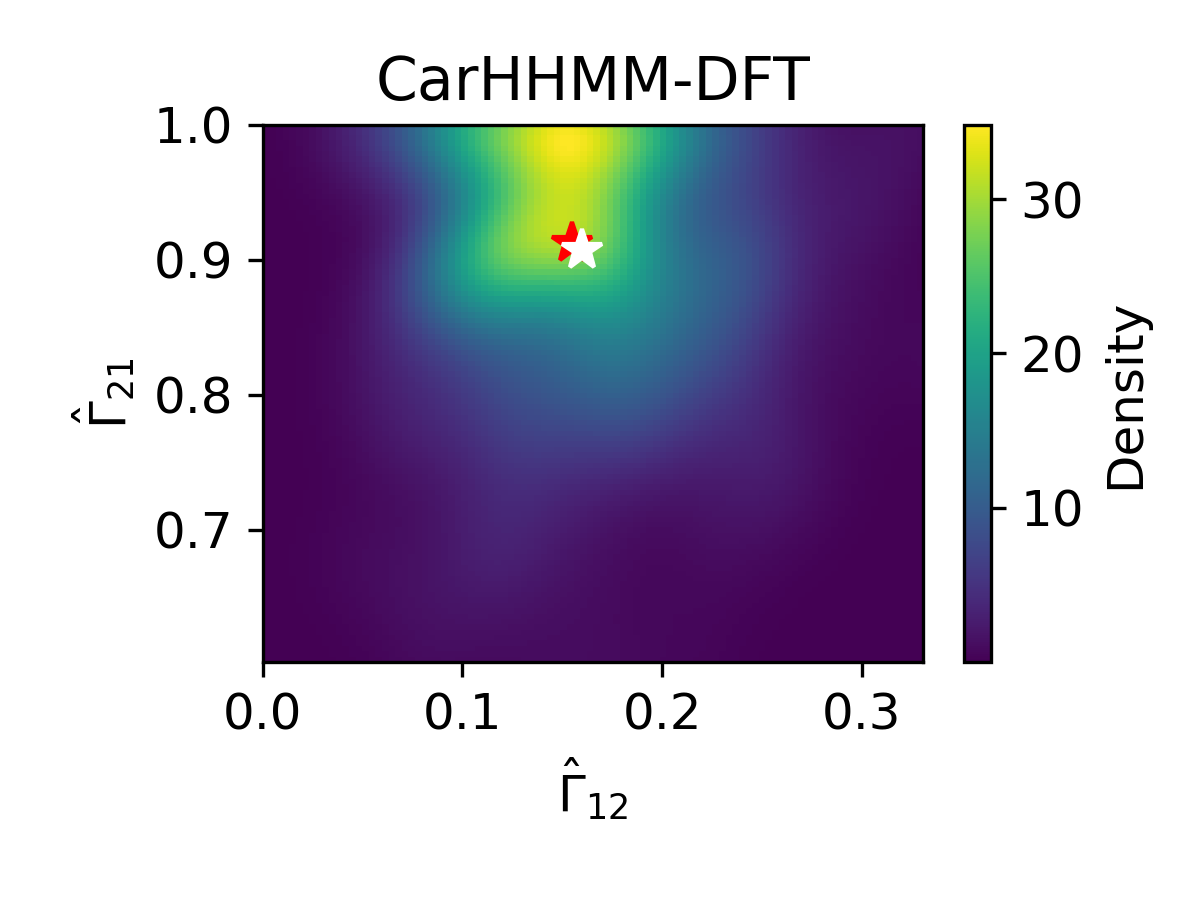
\includegraphics[width=2.5in]{../Plots/hhmm_FV_Gamma_density_-1_row_-1.png}
        
        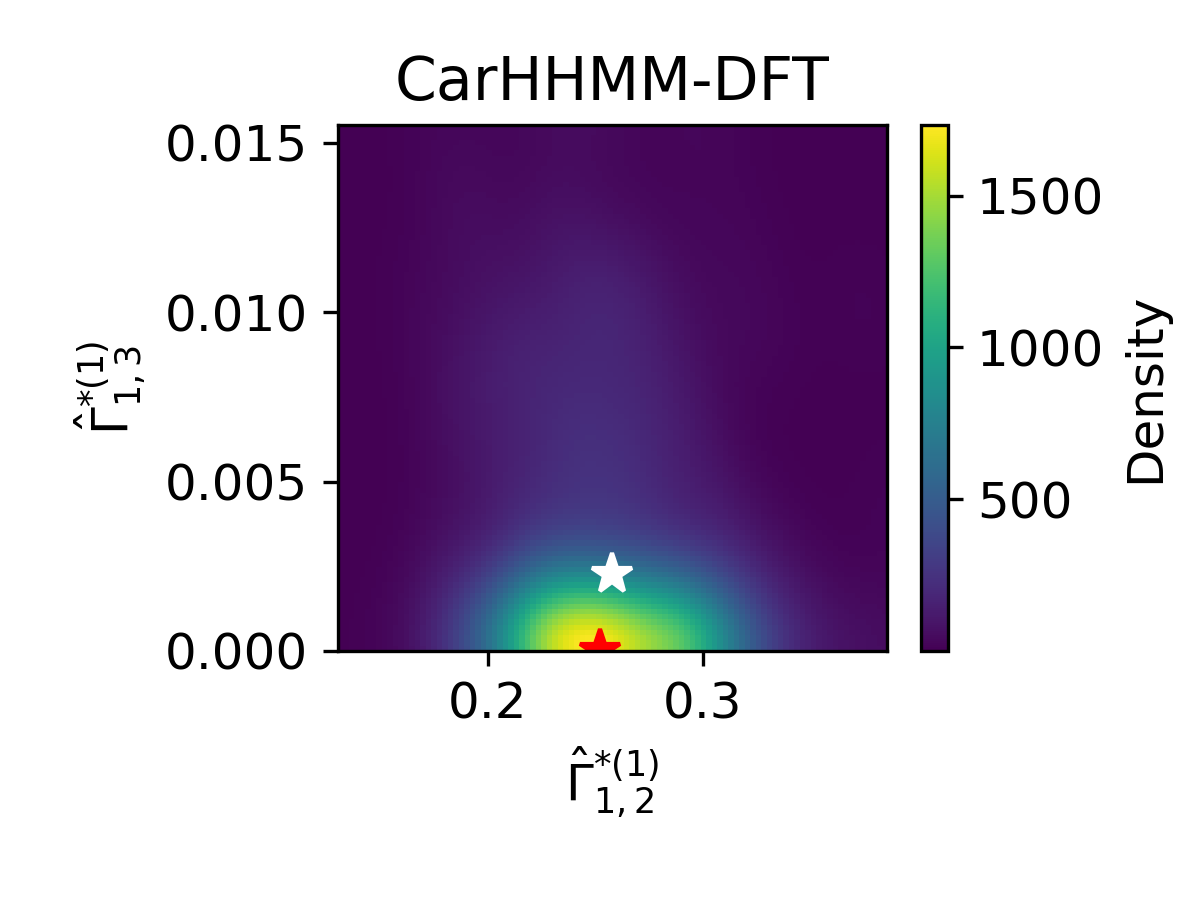
\includegraphics[width=2.5in]{../Plots/hhmm_FV_Gamma_density_0_row_0.png}
        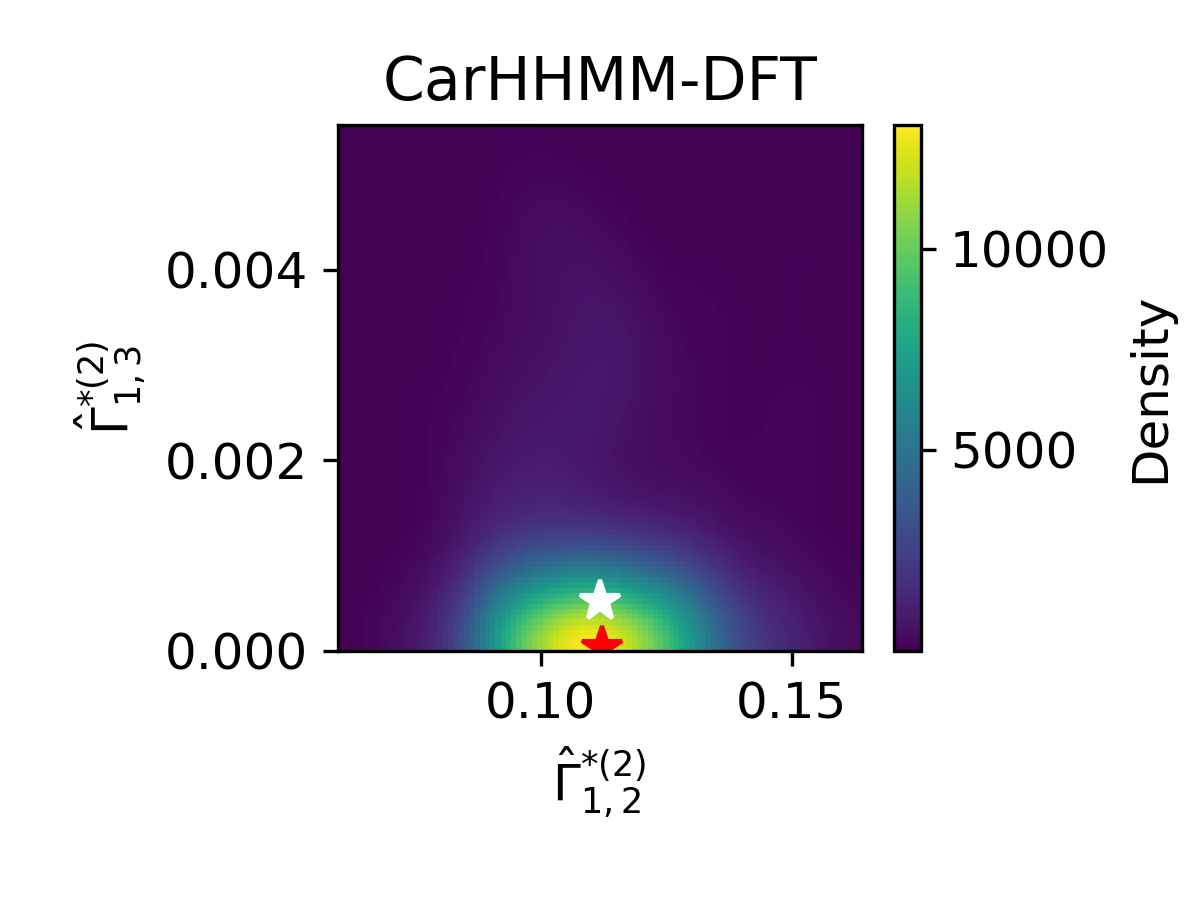
\includegraphics[width=2.5in]{../Plots/hhmm_FV_Gamma_density_1_row_0.png}
        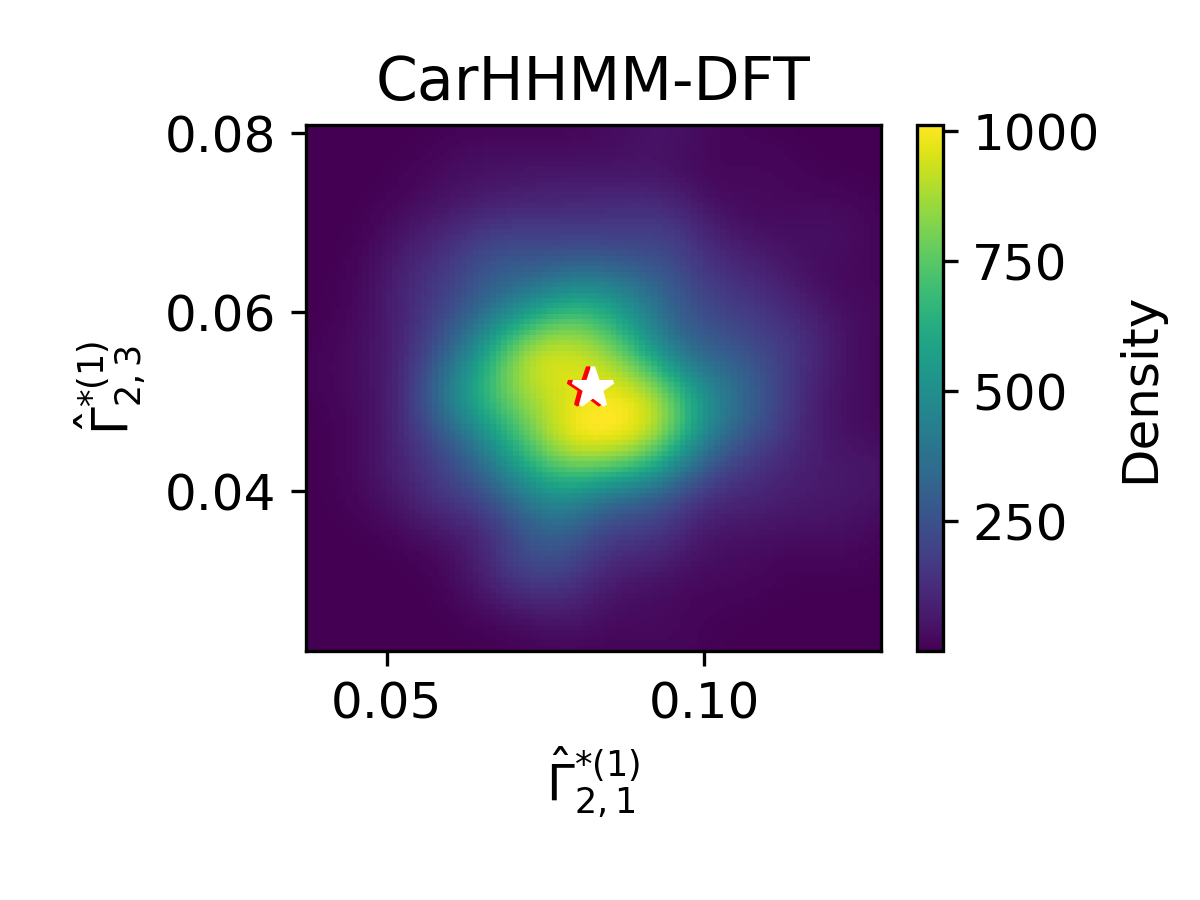
\includegraphics[width=2.5in]{../Plots/hhmm_FV_Gamma_density_0_row_1.png}
        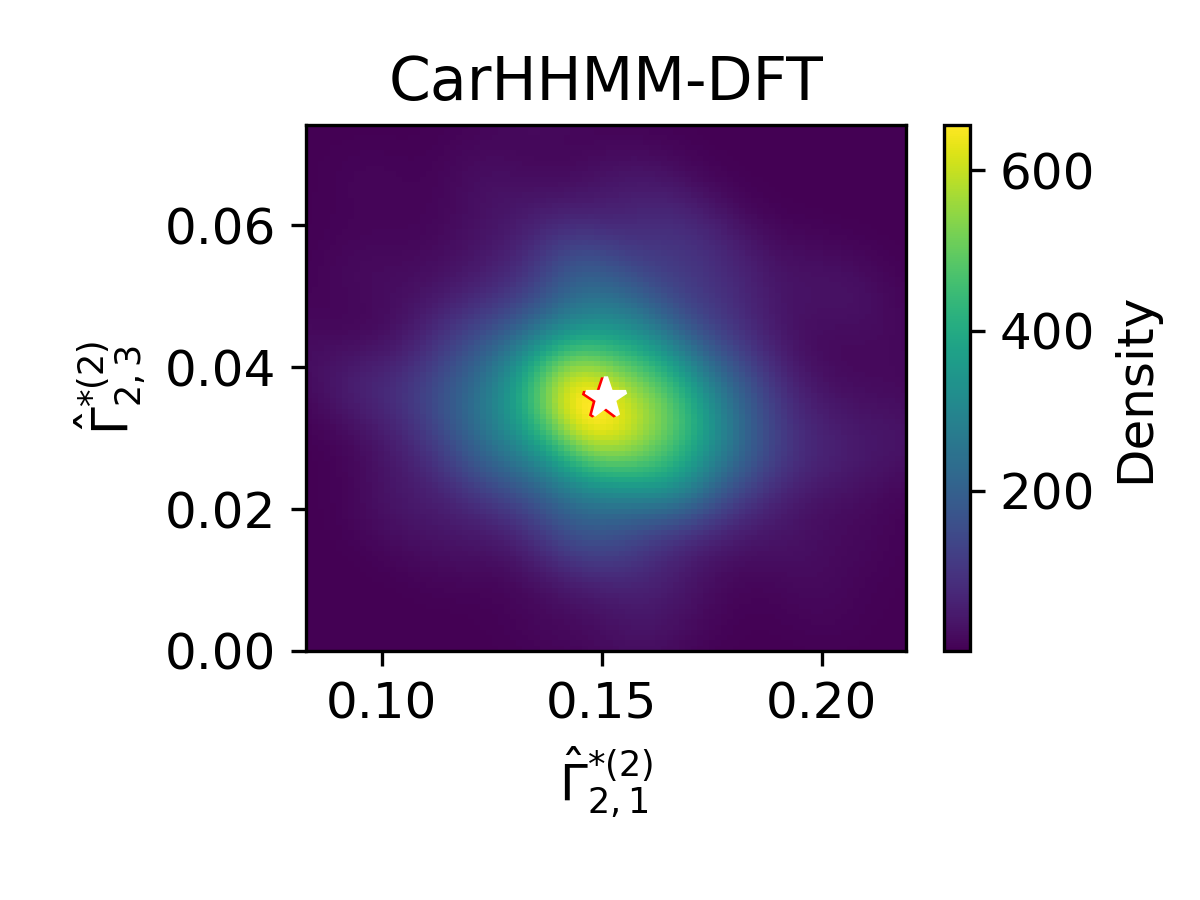
\includegraphics[width=2.5in]{../Plots/hhmm_FV_Gamma_density_1_row_1.png}
        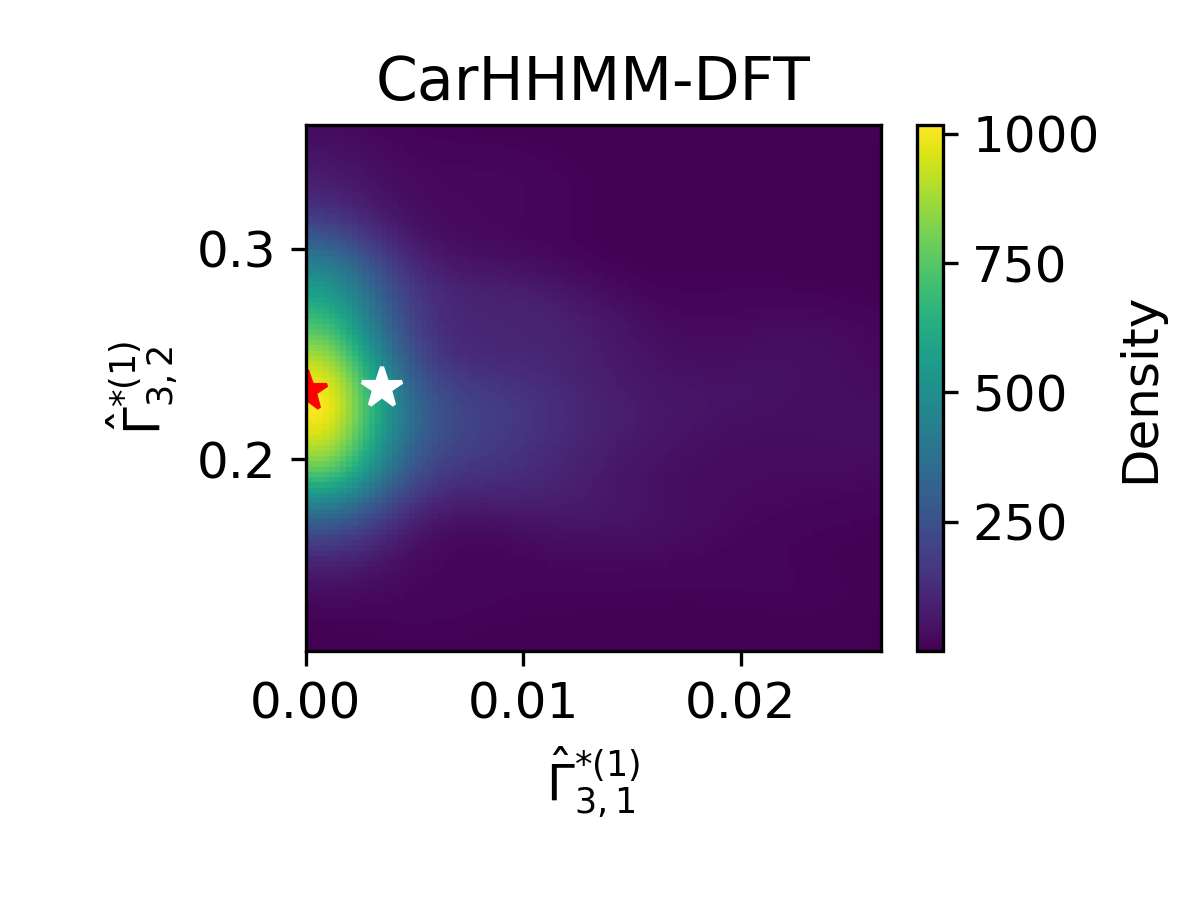
\includegraphics[width=2.5in]{../Plots/hhmm_FV_Gamma_density_0_row_2.png}
        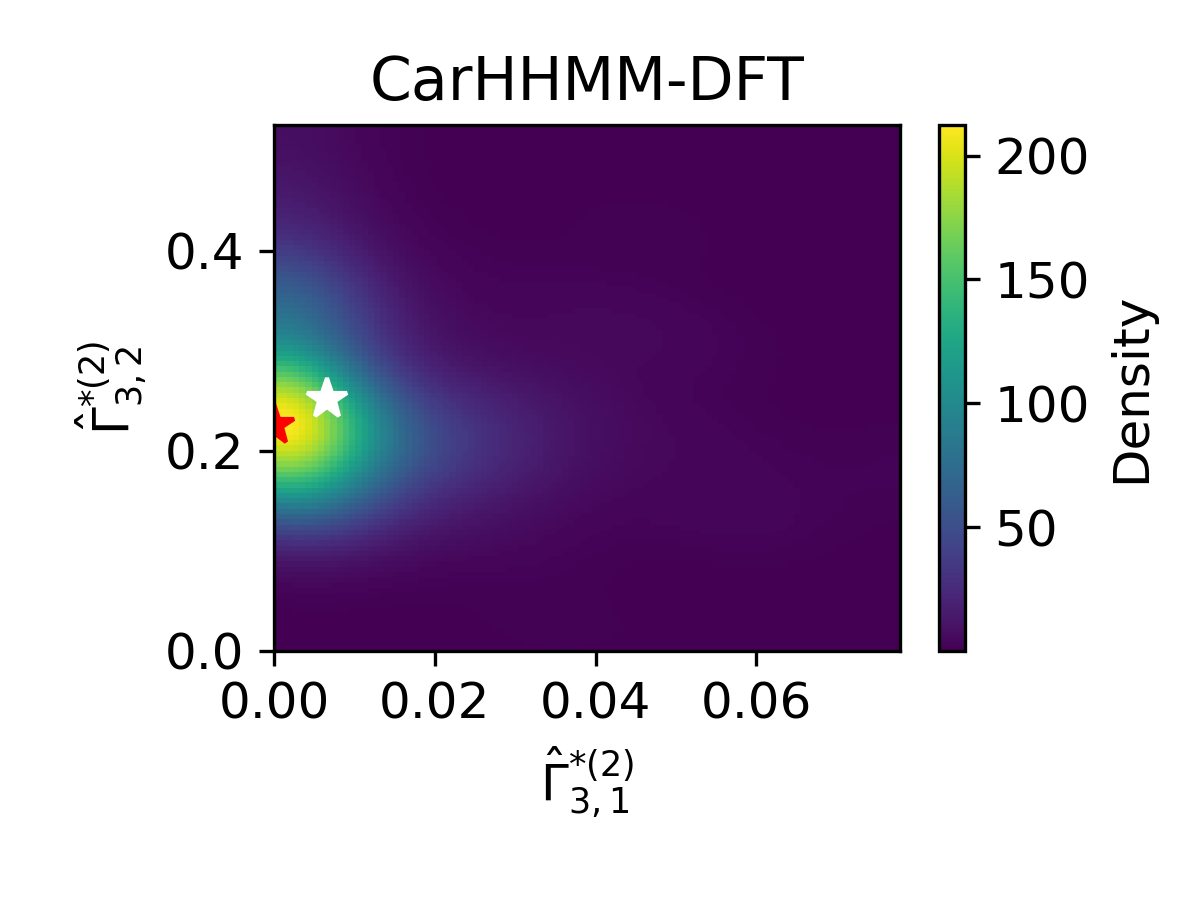
\includegraphics[width=2.5in]{../Plots/hhmm_FV_Gamma_density_1_row_2.png}
        \end{center}
        
        \noindent Figure \arabic{fignum}: Kernel density  estimates of the distributions of $\hat \Gamma$, $\hat \Gamma^{*(1)}$, and $\hat \Gamma^{*(2)}$ for the CarHHMM-DFT. There are two fine-scale probability transition matrices- one corresponding to each dive type. We only plot the off-diagonal elements of the probability transition matrices since this uniquely defines a stochastic matrix. The red star represents the true values and the white star represents the mean of all maximum likelihood estimates.
        \addtocounter{fignum}{1}
        
        \newpage
        \subsection{HHMM-DFT}
        \begin{center}
        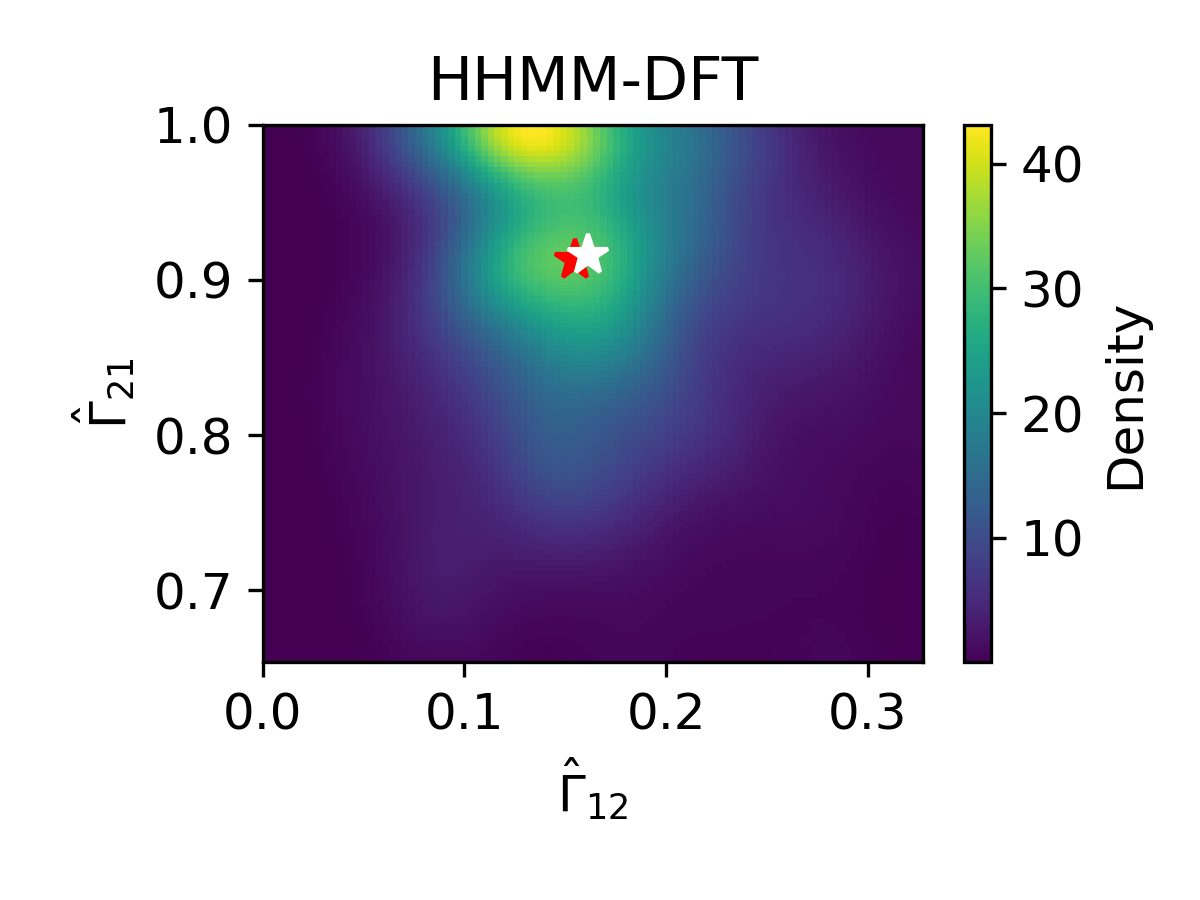
\includegraphics[width=2.5in]{../Plots/hhmm_FV_uncorr_Gamma_density_-1_row_-1.png}
        
        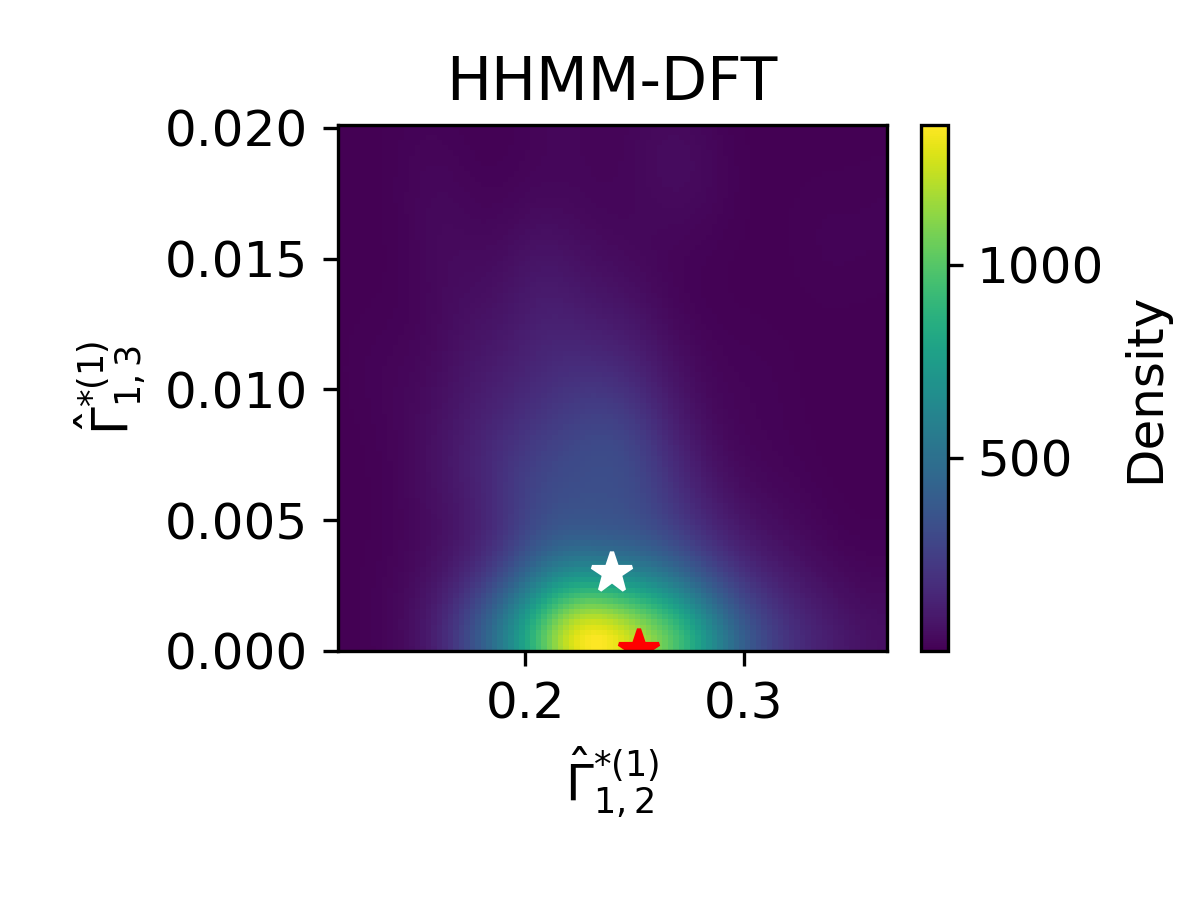
\includegraphics[width=2.5in]{../Plots/hhmm_FV_uncorr_Gamma_density_0_row_0.png}
        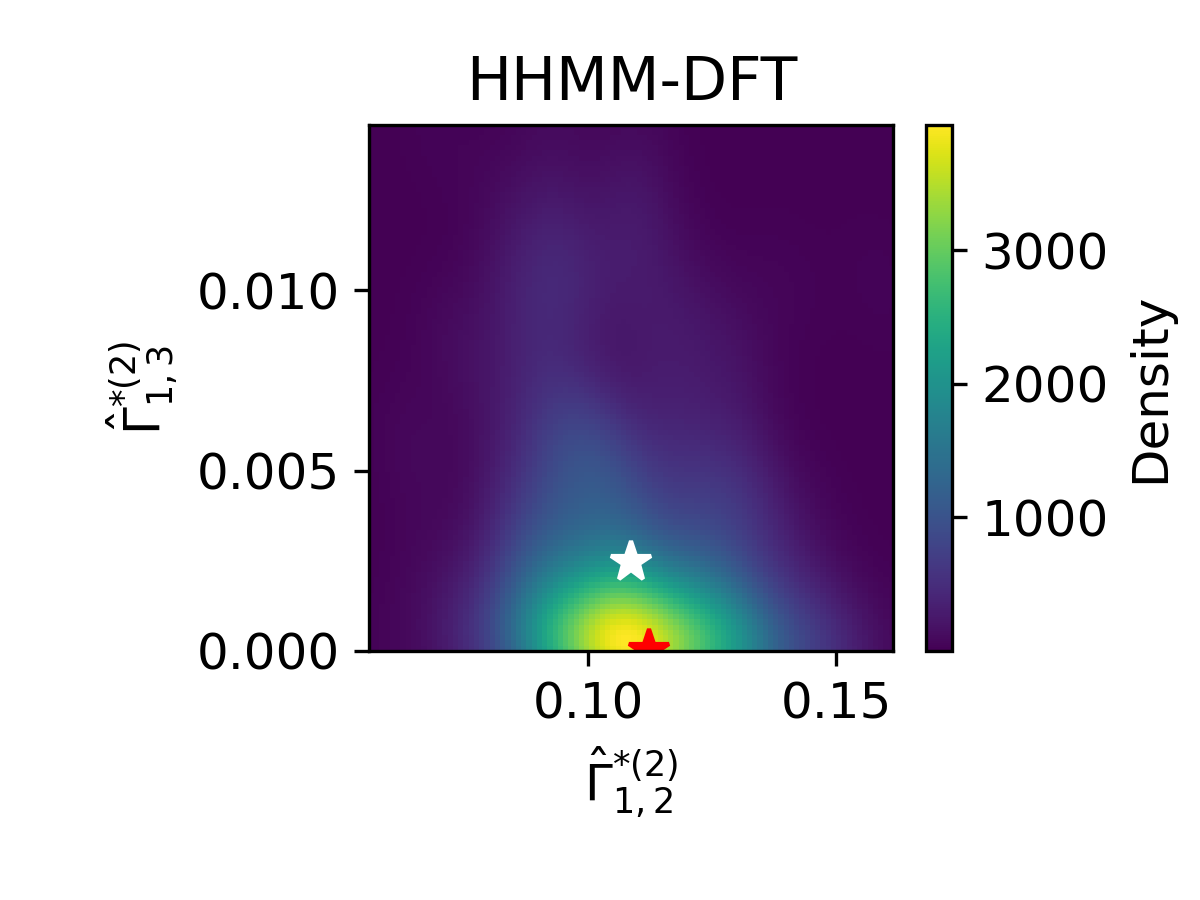
\includegraphics[width=2.5in]{../Plots/hhmm_FV_uncorr_Gamma_density_1_row_0.png}
        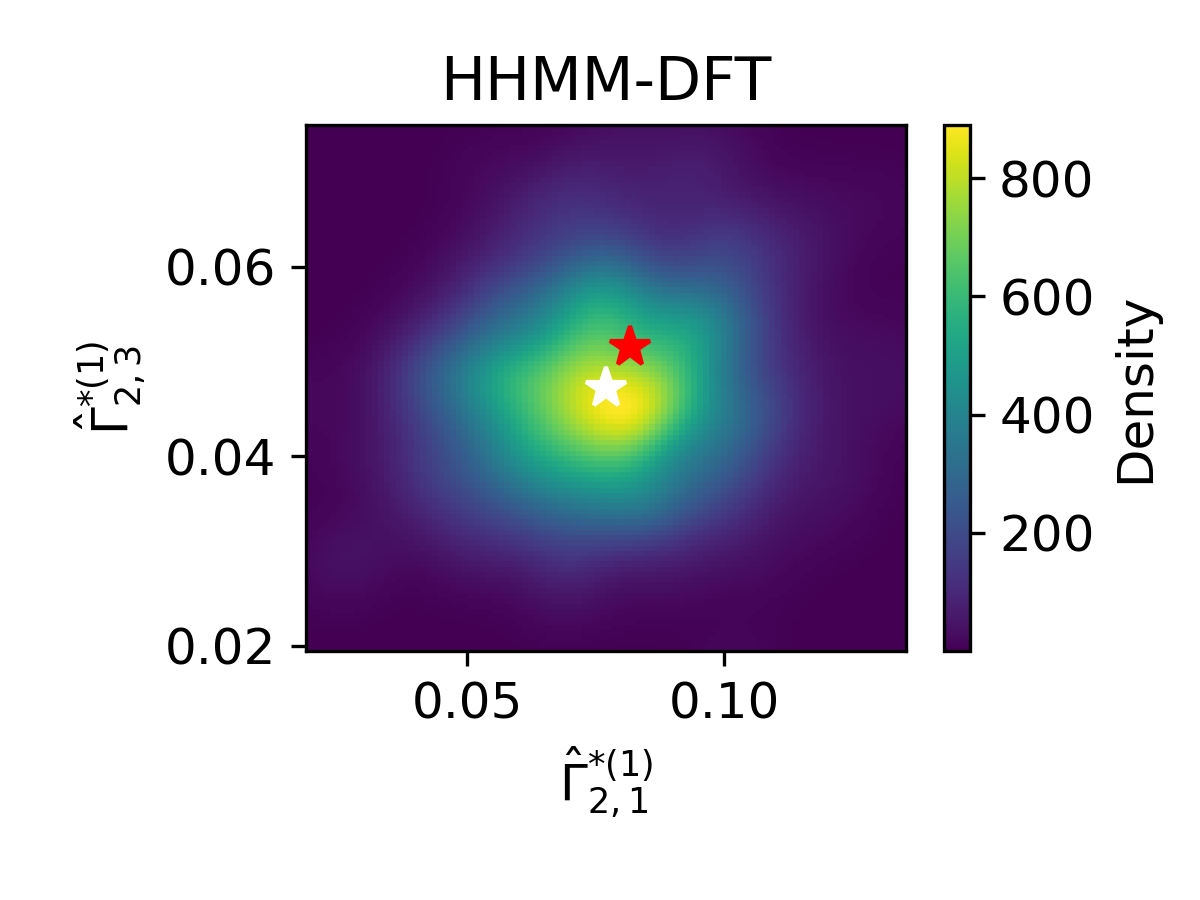
\includegraphics[width=2.5in]{../Plots/hhmm_FV_uncorr_Gamma_density_0_row_1.png}
        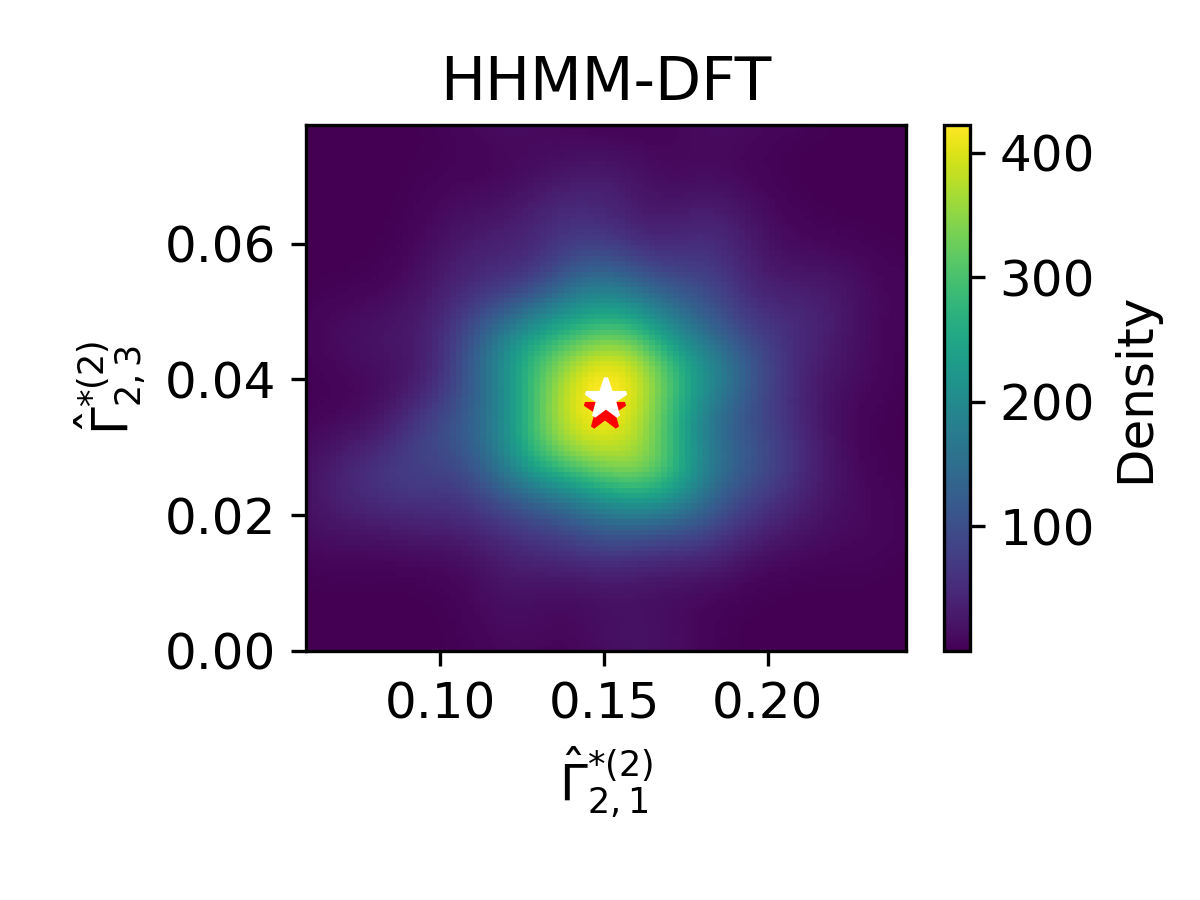
\includegraphics[width=2.5in]{../Plots/hhmm_FV_uncorr_Gamma_density_1_row_1.png}
        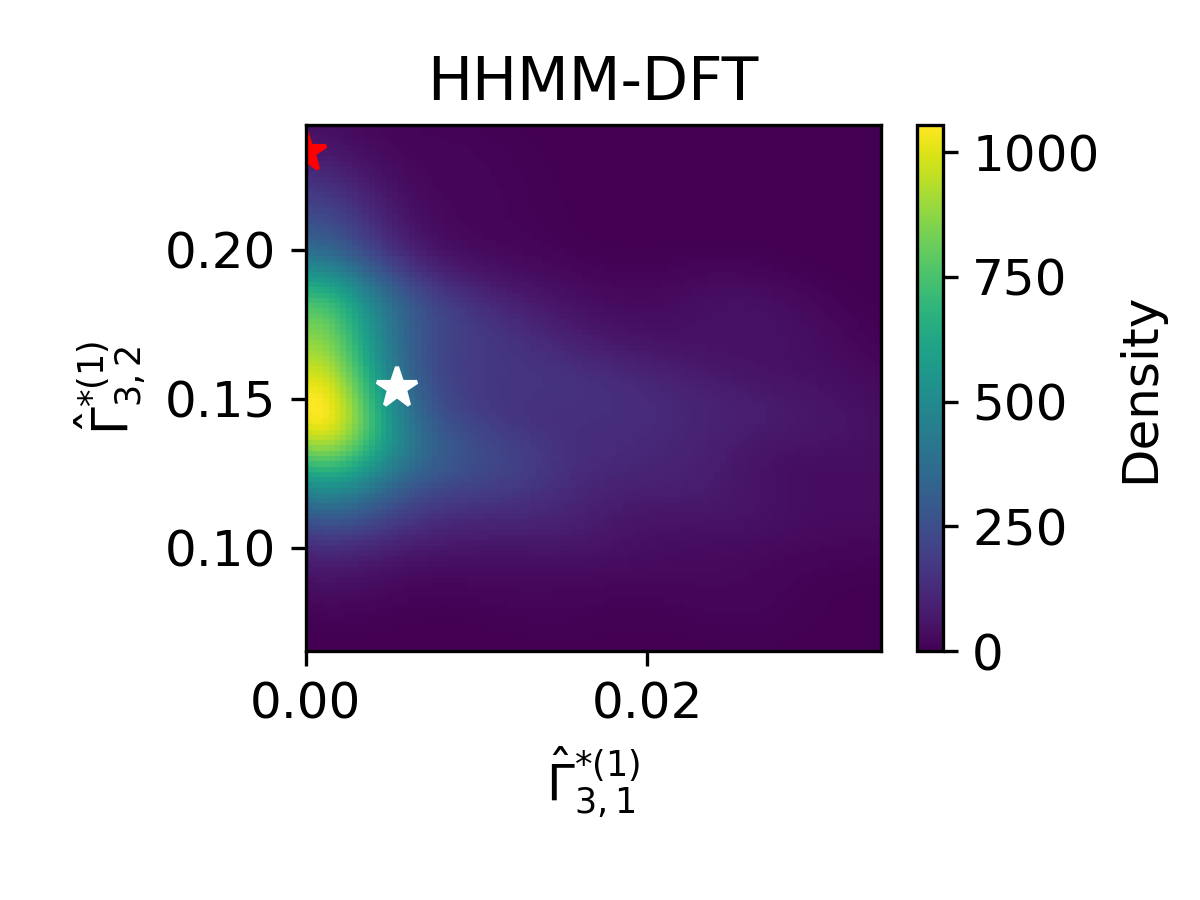
\includegraphics[width=2.5in]{../Plots/hhmm_FV_uncorr_Gamma_density_0_row_2.png}
        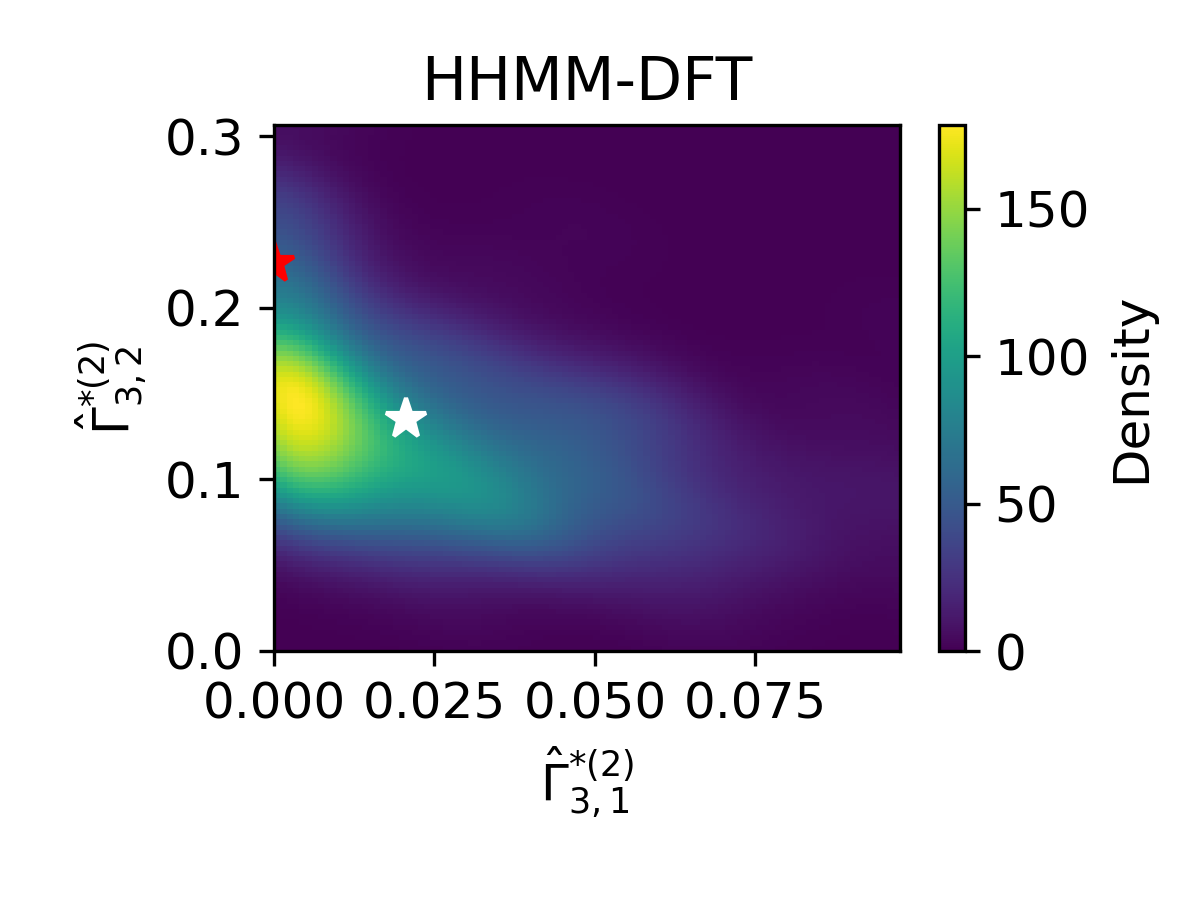
\includegraphics[width=2.5in]{../Plots/hhmm_FV_uncorr_Gamma_density_1_row_2.png}
        \end{center}
        
        \noindent Figure \arabic{fignum}: Kernel density  estimates of the distributions of $\hat \Gamma$, $\hat \Gamma^{*(1)}$, and $\hat \Gamma^{*(2)}$ for the HHMM-DFT. There are two fine-scale probability transition matrices- one corresponding to each dive type. We only plot the off-diagonal elements of the probability transition matrices since this uniquely defines a stochastic matrix. The red star represents the true values and the white star represents the mean of all maximum likelihood estimates.
        \addtocounter{fignum}{1}
        
        \newpage
        \subsection{CarHHMM}
        \begin{center}
        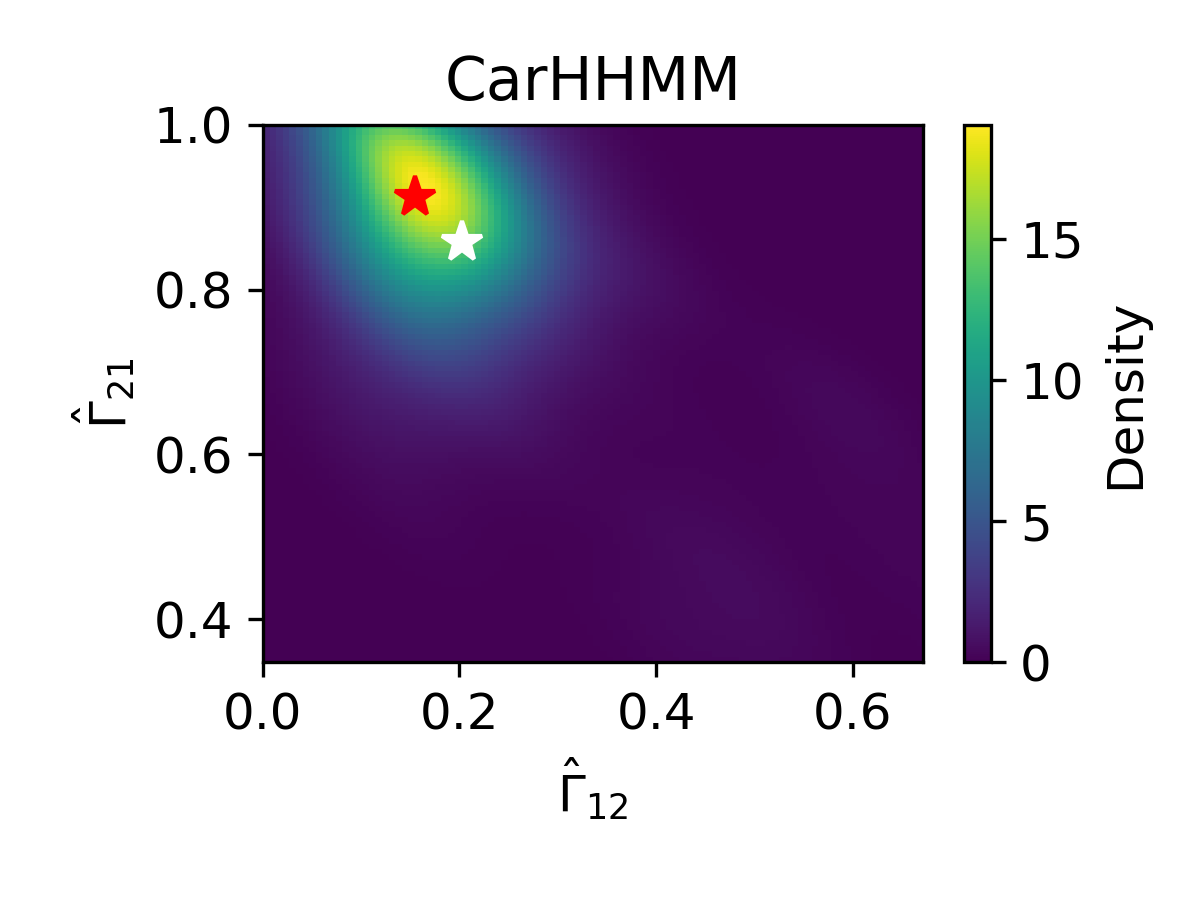
\includegraphics[width=2.5in]{../Plots/hhmm_V_Gamma_density_-1_row_-1.png}
        
        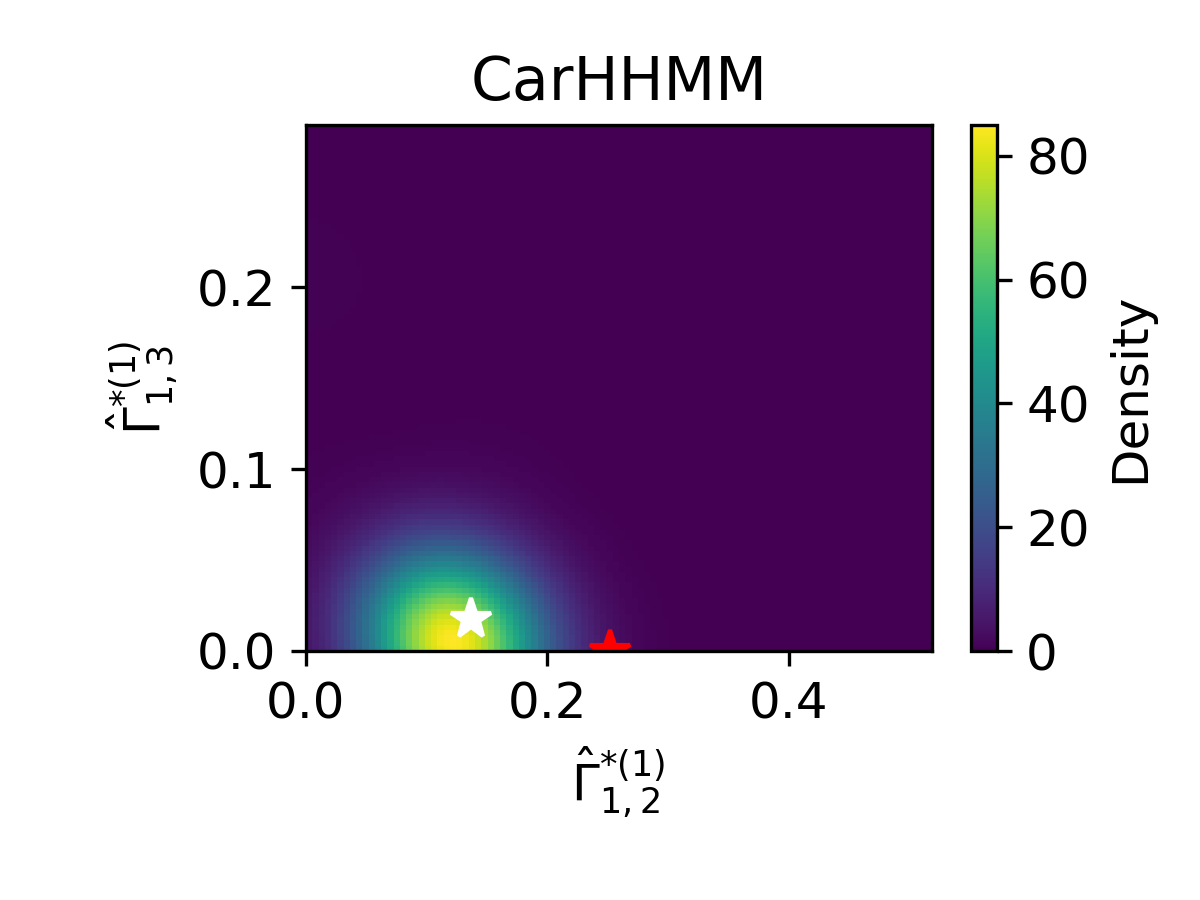
\includegraphics[width=2.5in]{../Plots/hhmm_V_Gamma_density_0_row_0.png}
        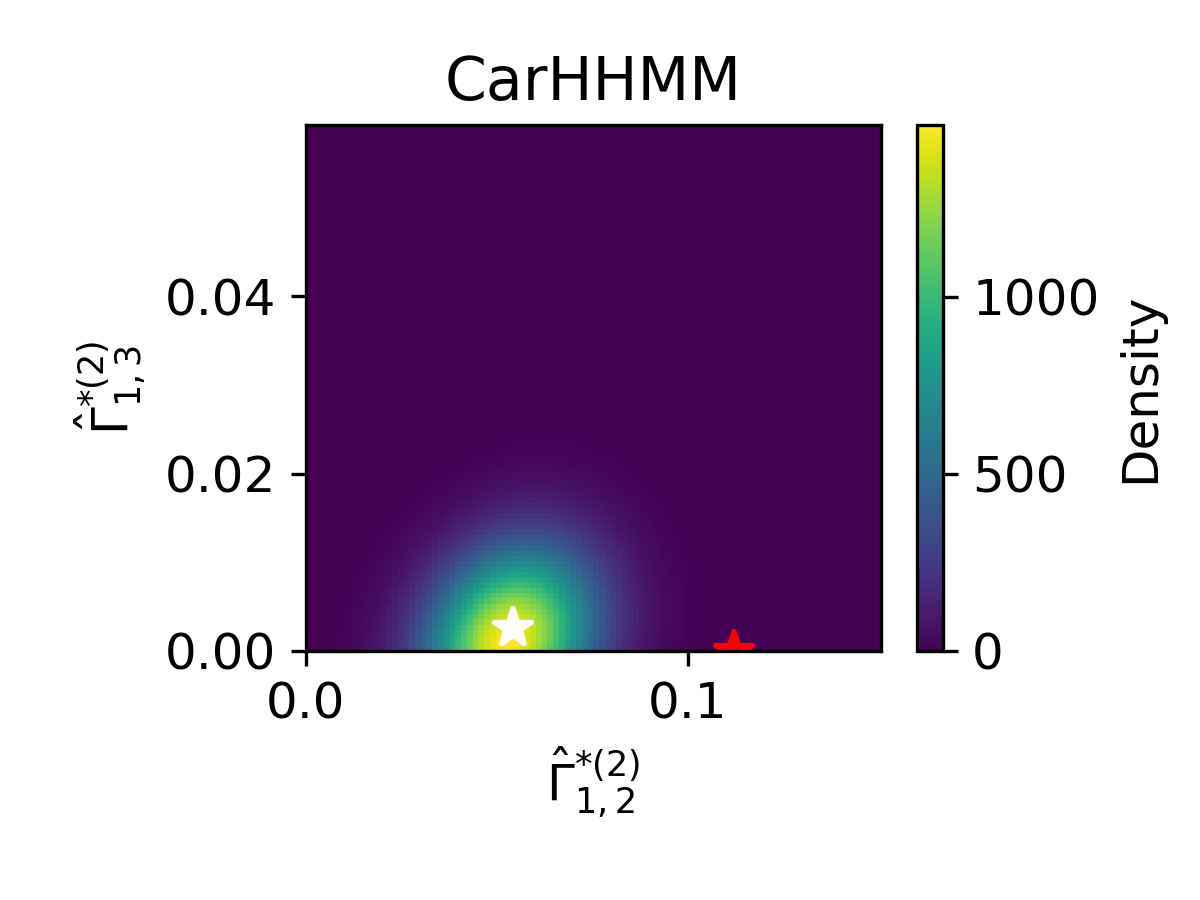
\includegraphics[width=2.5in]{../Plots/hhmm_V_Gamma_density_1_row_0.png}
        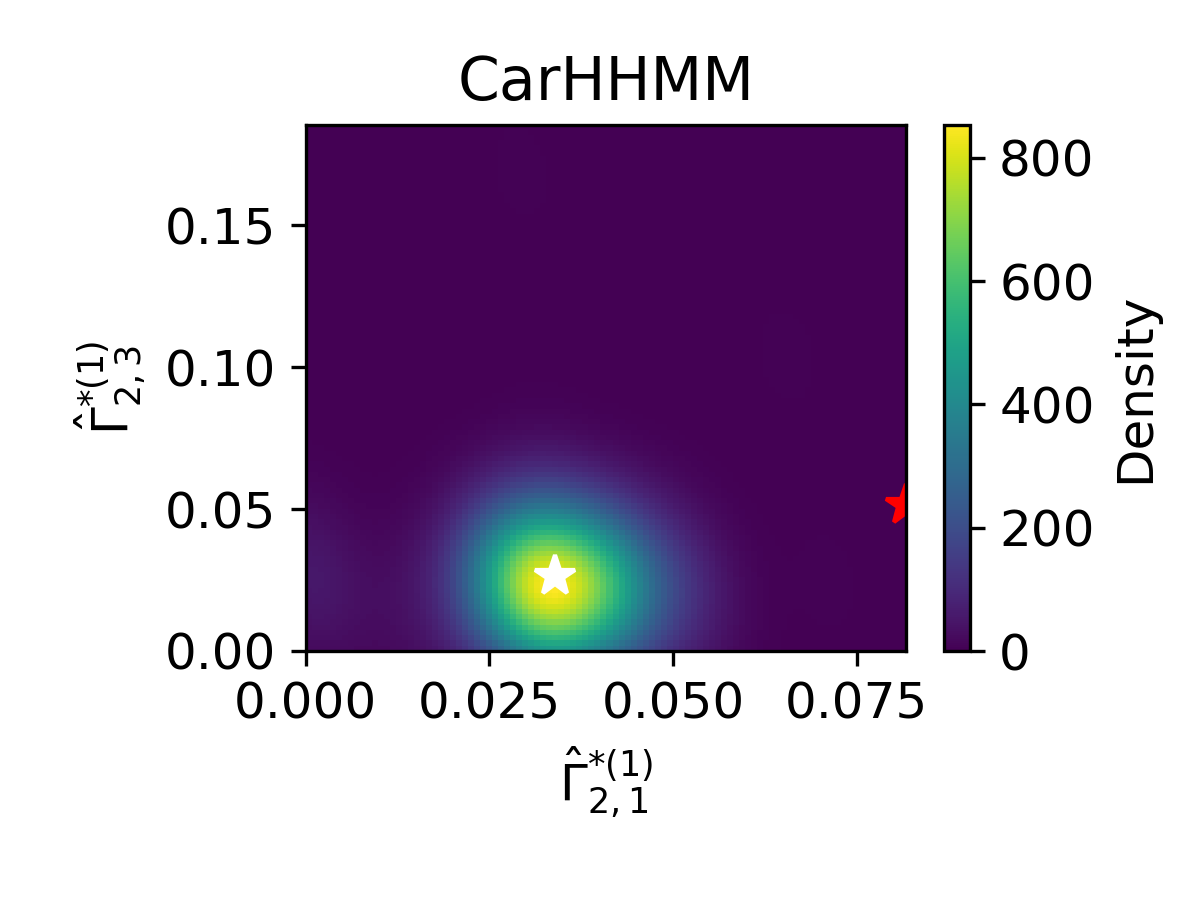
\includegraphics[width=2.5in]{../Plots/hhmm_V_Gamma_density_0_row_1.png}
        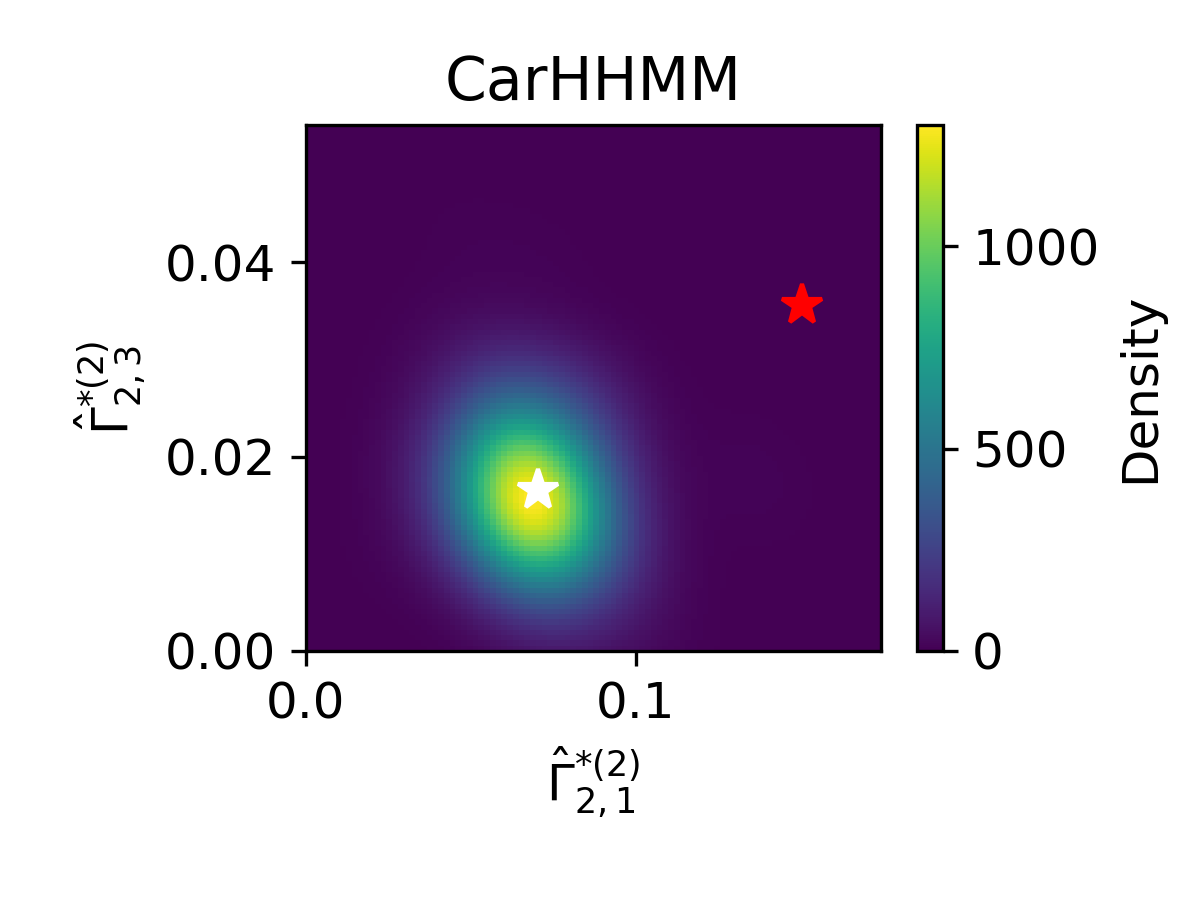
\includegraphics[width=2.5in]{../Plots/hhmm_V_Gamma_density_1_row_1.png}
        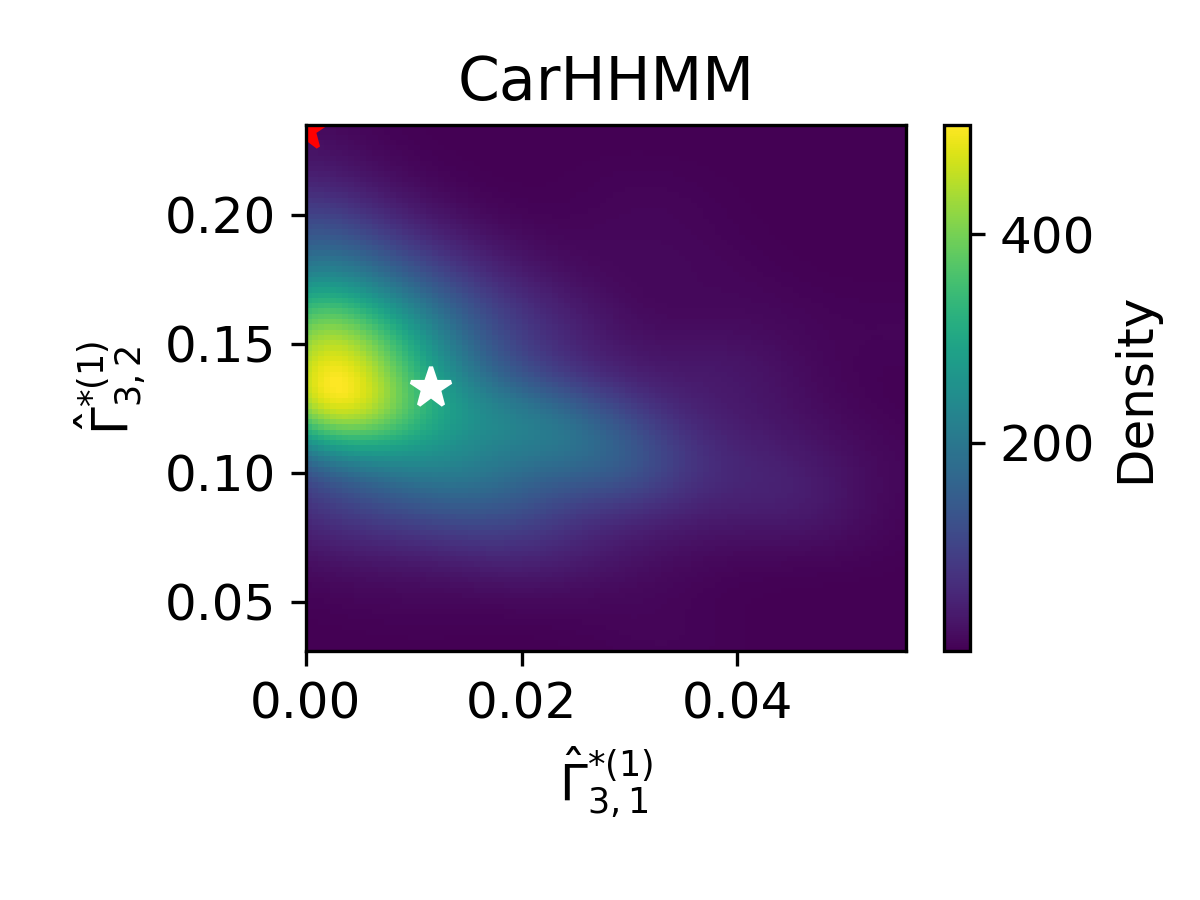
\includegraphics[width=2.5in]{../Plots/hhmm_V_Gamma_density_0_row_2.png}
        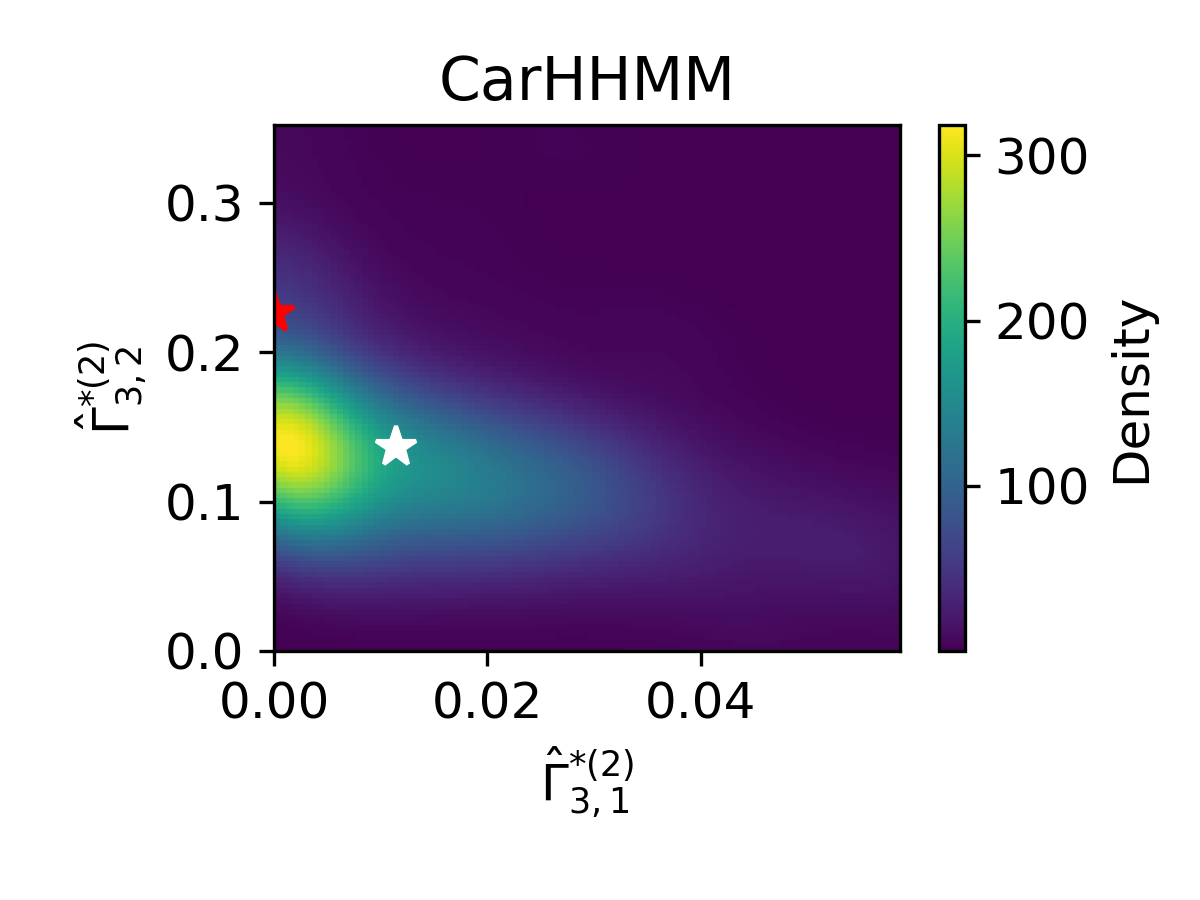
\includegraphics[width=2.5in]{../Plots/hhmm_V_Gamma_density_1_row_2.png}
        \end{center}
        
        \noindent Figure \arabic{fignum}: Kernel density  estimates of the distributions of $\hat \Gamma$, $\hat \Gamma^{*(1)}$, and $\hat \Gamma^{*(2)}$ for the CarHHMM. There are two fine-scale probability transition matrices- one corresponding to each dive type. We only plot the off-diagonal elements of the probability transition matrices since this uniquely defines a stochastic matrix. The red star represents the true values and the white star represents the mean of all maximum likelihood estimates.
        \addtocounter{fignum}{1}
        
        \newpage
        \subsection{CarHMM-DFT}
        \begin{center}
        \includegraphics[width=2.5in]{../Plots/hmm_FV_Gamma_density_0_row_0.png} \\
        \includegraphics[width=2.5in]{../Plots/hmm_FV_Gamma_density_0_row_1.png} \\
        \includegraphics[width=2.5in]{../Plots/hmm_FV_Gamma_density_0_row_2.png} \\
        \end{center}
        
        \noindent Figure \arabic{fignum}: Kernel density estimate of the distribution $\hat \Gamma^{*(1)}$ for the CarHMM-DFT. There is only one fine-scale probability transition matrix and no coarse-scale probability transition matrix since we assume that there is only one dive type for the CarHMM-DFT. We only plot the off-diagonal elements of the probability transition matrices since this uniquely defines a stochastic matrix. There is no red star which represents the true values because the CarHMM-DFT assumes that there is only one dive type.
        \addtocounter{fignum}{1}
\end{document}